\documentclass[a4paper,12pt]{book}

\pagestyle{myheadings}
\usepackage{blindtext}

\usepackage{pdfpages}
\usepackage{geometry}
\usepackage{newtxmath,newtxtext}
\usepackage{ragged2e}
\usepackage{indentfirst}
\usepackage{titlesec}
\usepackage[utf8x]{inputenc}
\usepackage[romanian]{babel}
\usepackage{combelow}
\usepackage{newunicodechar}
\usepackage{graphicx}
\usepackage{float}
\usepackage[procnames]{listings}

\usepackage{xcolor}

\definecolor{codegreen}{RGB}{166,226,46}
\definecolor{codegray}{rgb}{0.5,0.5,0.5}
\definecolor{codepurple}{rgb}{0.58,0,0.82}
\definecolor{backcolour}{rgb}{0.95,0.95,0.92}
\definecolor{darkblue}{rgb}{0.0,0.0,0.6}
\definecolor{comments}{RGB}{153,71,31}
\definecolor{returnc}{RGB}{174,129,255}

\usepackage[nottoc]{tocbibind}

\lstdefinestyle{mystyle}{ 
	frame = single,
	commentstyle=\color{comments},
	keywordstyle=\color{darkblue},
	numberstyle=\color{codegray},
	stringstyle=\color{codepurple},
	basicstyle=\ttfamily\footnotesize,
	breakatwhitespace=false,         
	breaklines=true,                 
	captionpos=b,                    
	keepspaces=true,                 
	numbers=left,                    
	numbersep=10pt,                  
	showspaces=false,                
	showstringspaces=false,
	showtabs=false,                  
	tabsize=4,
	procnamekeys={def,class},
	procnamestyle=\color{comments},
	%
	literate={pyauddio}{{\textcolor{green}{pyauddio}}}{8}%
	,
	emph={%  
		downto, for, with, self, None, lambda, True, False %
	},emphstyle={\color{darkblue}}%
}

\lstset{style=mystyle}

\graphicspath{ {../Diagrams/} }
\usepackage[font=small,labelfont=bf]{caption}
\newunicodechar{Ș}{\cb{S}}
\newunicodechar{ș}{\cb{s}}
\newunicodechar{Ț}{\cb{T}}
\newunicodechar{ț}{\cb{t}}
\newunicodechar{ă}{\u{a}}
\raggedbottom
\geometry{
	top 	= 2.5cm,
	bottom 	= 2cm,
	inner 	= 2.75cm,
	outer 	= 2cm,
	bindingoffset=0cm,
	headsep = 0.5cm,
	headheight = 0.5cm,
	footskip = 1cm,
}
\title{Lucrare Licenta}
\author{Steleac Raul-Dacian}

\titleformat{\chapter}
{\normalfont\fontsize{20}{14}\bfseries\sffamily}{\thechapter}{1em}{}
\titleformat{\section}
{\normalfont\fontsize{16}{14}\bfseries\sffamily}{\thesection}{1em}{}
\titleformat{\subsection}
{\normalfont\fontsize{14}{14}\bfseries\sffamily}{\thesubsection}{1em}{}

\titlespacing{\chapter}{0cm}{00pt}{30pt}
\titlespacing{\section}{0cm}{40pt}{20pt}
\titlespacing{\subsection}{0cm}{20pt}{10pt}

%\let\OLDthebibliography\thebibliography
%\renewcommand\thebibliography[1]{
%	\OLDthebibliography{#1}
%	\setlength{\parskip}{0pt}
%	\setlength{\itemsep}{0pt plus 0.3ex}
%}
\newcounter{Figcount}


\usepackage[maxbibnames=1,natbib=true,style=numeric,sorting=none,backend=bibtex]{biblatex}
\DeclareBibliographyCategory{cited}
\AtEveryCitekey{\addtocategory{cited}{\thefield{entrykey}}} 
\newcommand{\size}[2]{{\fontsize{#1}{0}\selectfont#2}}
\newenvironment{sizepar}[2]
{\par\fontsize{#1}{#2}\selectfont}
{\par}
\usepackage{filecontents}

\bibliography{Bibliography}
\nocite{*}

\renewcommand{\lstlistingname}{Algoritm}

\begin{document}
	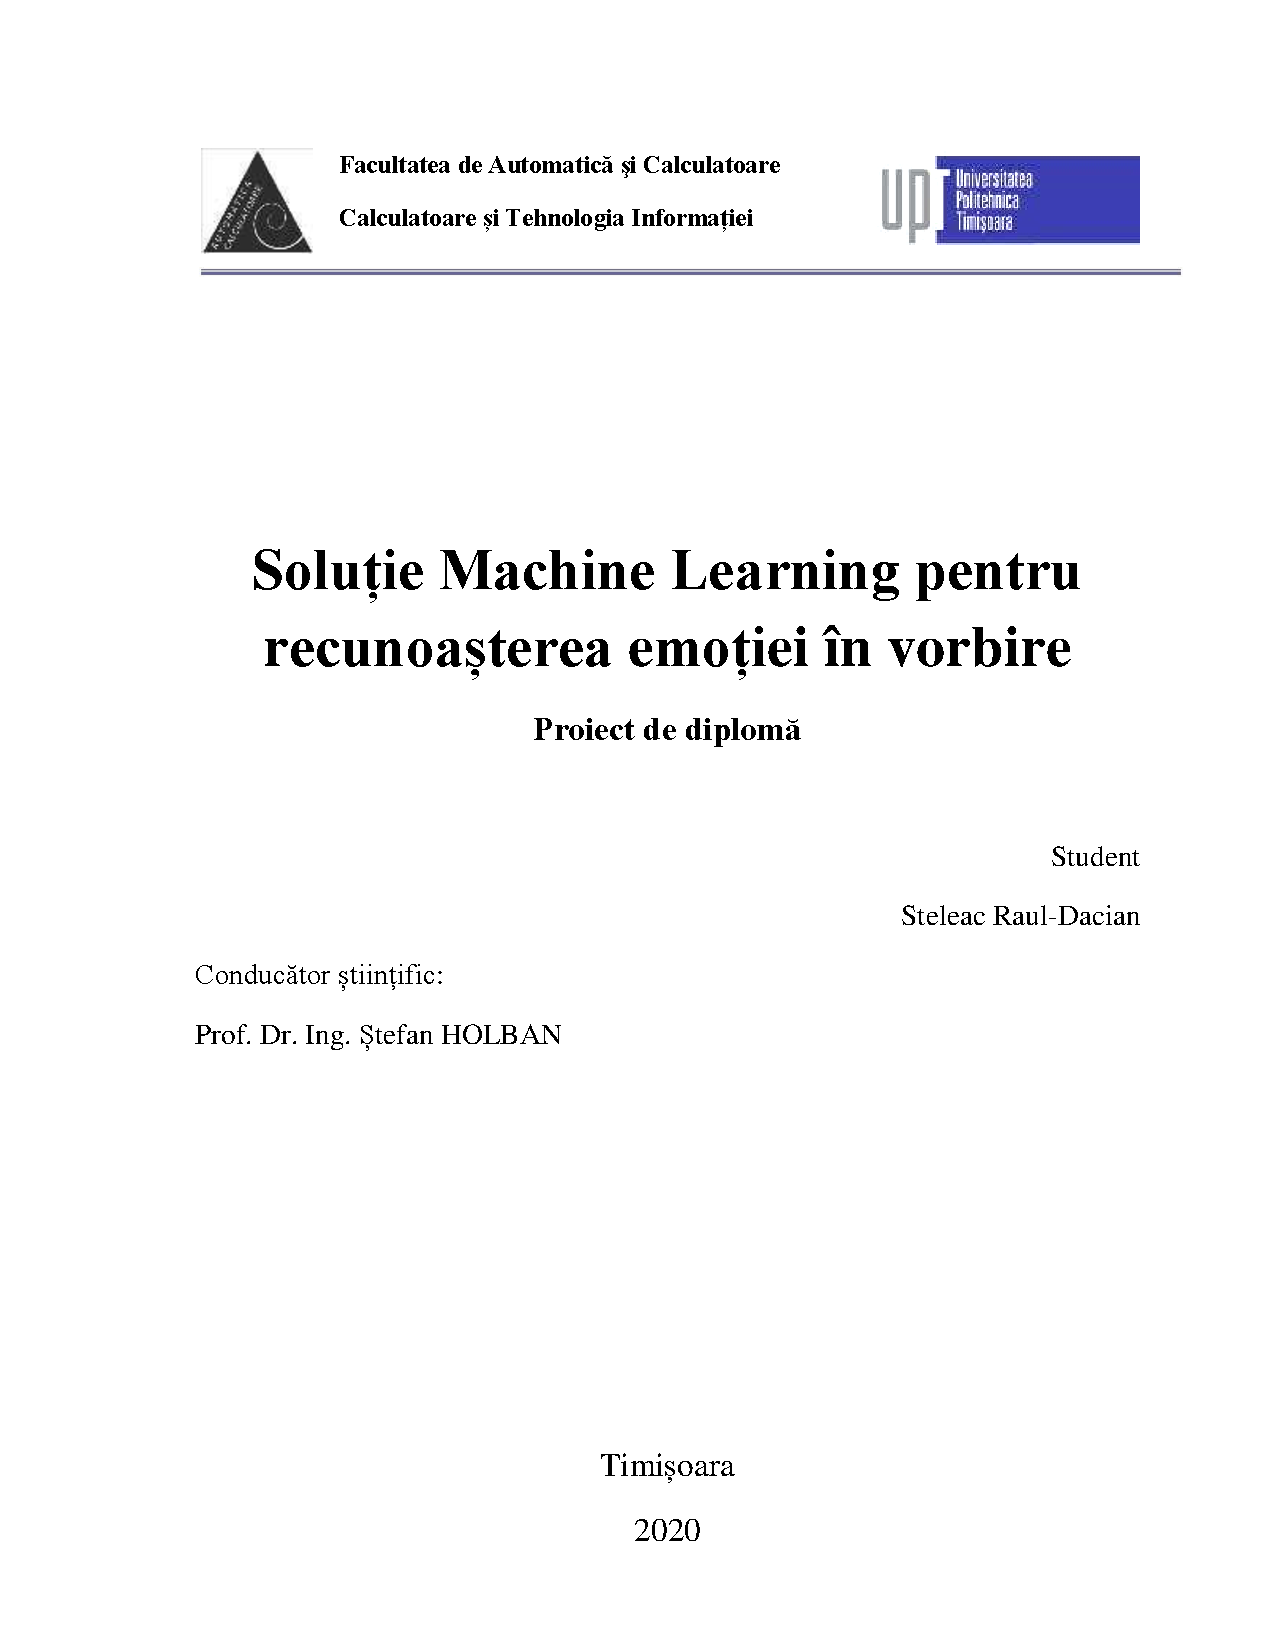
\includepdf{title_page}
	\clearpage
	\thispagestyle{empty}
	\tableofcontents
	\thispagestyle{empty}
	\clearpage
	\newpage 
	\thispagestyle{empty}
	
	\chapter{Introducere}
	
		\section{Prezentarea Problemei}
						
			\setlength{\parindent}{0.8cm}
			
			Comunicarea este o capacitate esențială pentru specia umană, fiind cea mai naturală și principala modalitate de transmitere a informației într-un mod direct. Totuși pe lângă informația lingvistică o mare parte din informațiile prezente în conversațiile pe care le avem zilnic sunt ascunse în emoțiile cu care rostim și articulăm diferite cuvinte, silabe și chiar litere. Urechea umană este capabilă să determine și cele mai mici inflexiuni din vocile participanțiilor la conversație pentru a reuși să capteze cât mai bine sensul acesteia. Astfel, este de așteptat că mașinile care urmează să facă parte de acum din aceste conversații să fie la fel de competențe din această privința. Domeniul stintific care se ocupă cu crearea unor modele de tip "Machine Learning" pentru determinarea emoțiilor dintr-un discurs se numește "Speech Emotion Recognition", sau SER. \par
			
			Proiectul de diplomă propus de mine încearcă să creeze o soluție pentru recunoașterea emoției în vorbire și să ofere un mediu de utilizare propice printr-o interfață grafică care conține diferite funcționalități de configurare a modelului, extragere de statistici și înregistrare. Utilizatorul are astfel opțiunea de a antrena soluția SER propusă de mine cu diferite configurații de parametrii cât și de a testa modelul obținut pe semnale audio pre-înregistrate sau înregistrate pe loc.\par
			
			\subsection{Importanța informației emoționale}
				Informația emoțională este prezentă în orice conversație și reprezintă un punct de reper către sensul din spatele cuvintelor vorbitorilor. Emoțiile pot pe de o parte să adâncească sensul unor anumite cuvinte sau chiar să îl întoarcă pe dos dacă sunt folosite în ipostaze contradictorii. De exmeplu, propozițiile sumbre ar putea fi considerate glume dacă sunt rostite într-un mod umoristic la un moment potrivit sau propozițiile pozitive pot să devină sarcastice pe un ton trist. Un participant la conversație care nu poate să înțeleagă aceste concepte va fi astfel puternic dezavantajat. Deoarece oamenii sunt mai mult sau mai puțin experți în determinarea acestor informații emoționale, dorim ca și viitoarea generație de vorbitori, agenții AI, să poată să realizeze această performanță.\par
				În trecut, majoritatea studiilor legate de rolul emoției umane în acustica unui discurs au fost făcute în psihologie. Blanton, 1915 \cite{blanton}, de exemplu, a scris că efectul emoției asupra intonațiilor vocii sunt recunsocute de orice persoană. Chiar și cele mai primitive specii pot recunoaște tonuri care reprezintă dragoste, frică sau enervare (de exemplu, câinii, caii, și multe alte animale pot înțelege părți din limbajul uman), limbajul tonurilor fiind cel mai vechi și universal dintre toate modurile de comunicare.\par 
				Plecând de la motivația că informația emoțională  este folosită în mecanismul de comunicare chiar și a celor mai primitive specii, putem să ne întrebăm care era modalitatea de comunicare a strămoșilor noștrii înainte de apariția cuvintelor. Capacitatea obținerii unei forme de limbaj nu era posibilă pentru specia \textit{Homo erectus}, strămoșii speciei \textit{Homo sapiens}, deoarece dezvoltarea vorbirii a necesitat o conexiune directă a cortexului motor central cu mușchii intercostali , conexiune care lipsește din construcția coloanei vertebrale ale acestora. Prima specie din familia \textit{Hominidae} care s-au bucurat de acest beneficiu a fost \textit{Homo sapiens}.  Levinson \& Holler, 2014 \cite{leviholler} susțin convenția că limbajul a apărut cu aproximativ o sută de mii de ani după apariția speciei umane, \textit{Homo sapiens}, care se estimează a fi acum circa trei sute de mii de ani. Astfel printr-un calcul rapid puitem să determinăm că a existat o perioadă de circa o sută de mii de ani în care strămoșii noștri, \textit{Homo sapiens}, deși capabili să folosesaca un limbaj pentru comunicare, nu au făcut-o. Christiansen \& Kirby, 2003 \cite{chriskirbi} menționează un consens între cercetătorii acestui domeniu în legătură cu pașii necesari prin care o specie poate să dezvolte un limbaj. Mai exact, consensul este că înainte de apariția limbajului câteva "pre-adaptări" au trebuit să apară în descendenții familiei \textit{Hominidae}. Deși cercetătorii nu sunt complet de acord în legătură cu lista acestor "pre-adaptări", un candidat propus de majoritate a fost abilitatea de folosi așa numite "simboluri". În acest context, simbolurile reprezintă capacitatea de a crea legături între sunete și gesturi arbitrare cu anumite emoții, concepte sau percepții specifice. Aceste gesutri și sunete au alcătuit astfel primele forme de dialog al speciei umane. Putem să observăm astfel cum deși informația lingvistică nu există încă în comunicarea speciei umane, informația emoțională a fost inclusă încă de la primele forme de interacțiuni sociale.\par 				
				Cantitatea de informație din spatele emoțiilor pe care le folosim astăzi în limbajul modern rămâne la fel de importantă că pe vremea strămoșilor noștri. De aceea, în prezent, studiul importanței emoției dintr-o conversație este extins și în domeniul calculatoarelor prin inteligență artificială. \par 	
				
			\subsection{Domeniul recunoașterii emoției in vorbire}
				Domeniul "Speech Emotion Recognition", sau SER, are ca scop final construirea unui model de tip "Machine Learning" care să primească de la intrare o înregistrare audio, o parte dintr-o conversație, și să genereze la ieșire o emoție, care să fie reprezentativă pentru acea înregistrare. \par
				Recunoașterea emoțiilor în vorbire este o problema care a stârnit curiozitatea adepților domeniului inteligenței artificiale de câteva decenii. Daellert et al., 1996 \cite{dellaert} au deschis granițele acestui domeniu în 1996 cu primul articol stintific care încearcă să combată acest subiect. Aceștia au încercat să clasifice patru tipuri de emoții prin folosirea unor date de intrare așa numite "prosodice" ca tonalitatea, intensitatea, frecvența sau amplitudinea folosind trei tipuri de modele de clasificare diferite "Maximum Likelihood Bayes classifier" (MLB), "Kernel Regression"  (KR) și "K-nearest neighbors" (KNN). Această implementare este una reprezentativă pentru combaterea recunoașterii de emoții în vorbire, realizând o separare clară între cele două module arhitecturale principale: extragerea datelor și clasifiactorul care urmează să fie antrenat. Discrepanța dintre arhitecturile folosite în prezent și cea prezentată mai sus rămâne însă observabilă. Chiar dacă datele de intrare prosodice sunt încă folosite astăzi, creșterea drastică a puterii de procesare a dus la folosirea unor arhitecturi cu rețele neuronale adânci care adopta ori mai multe tipuri de date de intrare ori direct semnalul audio neprocesat, dacă modelul realizează extragerea datelor printr-o manieră automată, "end-to-end models". \par		
				
				Diferențele arhitecturale sunt totuși un semn benefic, fiind reprezentative pentru evoluția domeniului de cercetare. SER și-a păstrat popularitatea în ultimele două decenii dețînând un număr bogat de articole stintifice pe această tema. Aceste articole aduc noi interpretări atât din punctul de vedere al extragerilor caracteristicilor semnalului audio folosite ca date de intrare cât și a modelului folosit pentru antrenare. Totuși, deși noi idei și arhitecturi contiună să apară anual, această tehnologie nu a reușit să atingă încă o acuratețe destul de satisfăcătoare pentru a fi lansată pe piață. \par
				
				O tehnologie indrudita a recunoașterii emoției în vorbire, "Speech Recognition" care încearcă să determine informația lingvistică dintr-o conversație, a reușit să revoluționeze interfețele de comunicare dintre om și mașină. Această tehnologie își găsește locul în majoritatea telefoanelor, calculatoarelor, mașinilor și chiar a unor echipamente din jurul casei. Alexa, Cortana și Siri sunt câteva nume pe care majoritatea persoanelor le cunosc fără să le asocieze cu o față sau o persoană. Acești agenți inteligenți obțin rezultate excepționale în capacitatea lor de a menține o conversație cu clienții și de a răspunde la anumite cerințe ale acestora. Cu toate acestea, algoritmii de "Speech Recognition" nu resuesc mereu să răspundă corect la afirmațiile utilizatorilor deoarece nu iau în considerare și partea emotivă a dialogului. Pentru a obține o inerfata de comunicare om-mașină completă, informația emoțională este esențială. Prin diferite intonații sensul cuvintelor poate fi schimbat complet iar un algoritm care se focusează doar pe informația lingvistică va rămâne inflexibil la aceste intonații generând astfel rezultate eronate. \par
					

		\section{Motivația problemei}
		Recunoașterea emoției în vorbire reprezintă un subiect extrem de interesant atât din punct de vedere aplicativ cât și personal. Potențialul acestui domeniu este ridicat din cauza numărului ridicat de aplicații care pot beneficia prin încorporarea unui astfel de sistem. Modurile în care un sistem SER poate fi utilizat sunt limitate doar de nivelul tehnologic curent și imaginația programatorilor.
			\subsection{Motivație aplicativă}				
					Aplicațiile în care această tehnologie poate fi folosită în viitor sunt greu de estimat, deoarece orice interfață om-mașină care folosește dialogul ca modalitate de transmitere de informațîi poate beneficia prin includerea unui astfel de algoritm. Cu toate acestea, o gama largă de aplicații din prezent sunt deja succeptibile la a fi îmbunătățite prin intermediuli introducerii unui model SER. \par
					
					Un bun exemplu este încorporarea unui algoritm SER în mecanismul de \textit{"feed-back"} al unei companii. Principala modalitate prin care firmele din zilele noastre încearcă să capteze părerea publicului asupra unui produs este prin folosirea unor chestionare. Chiar dacă aceste chestionare iau loc în scris sau telefonic aduc anumite limitări. În prima situație apare incertitudinea asupra onestitățîi răspunsurilor oamenilor iar în cea de a două situație apare limitarea personalului disponibil care să asculte răspunsurile intervievatiilor în decursul chestionarului. Un sistem alcătuit dintr-un algoritm de "speech emotion recognition" împreună cu unul generic de "speech recognition" poate capta atât informația lingvistică cât și cea emoțională din răspunsurile la întrebările chestionarelor, notând atât cuvintele în sine cât și gradul de credibilitate bazat pe implicarea emoțională a participantului. \par
					
					Un alt exemplu ar fi implicarea modelelor SER în tehnologiile care ne ușurează deja viața de zi cu zi. Agențîi inteligenți și diferitele tipuri de roboți, ca de exemplu Huahu et al., 2010 \cite{huahu}, care apar tot mai des în prezent în apropierea oamenilor pot găsi un mare avantaj în determinarea emoțiilor clienților când încearcă să răspundă cât mai exact la nevoile acestora. De exemplu un astfel de agent inteligent încorporat într-o mașină poate detecta dacă în timpul mersului șoferul este implicat într-o ceartă sau o discuție cu un puternic impact emoțional. Dacă acest lucru este adevărat, sistemul SER poate să-l îndrume pe șofer să opreasa mașina până când discuția s-a terminat in scopul evitării unui accident din cauza lipsei de atenție. Alexa sau Siri, care sunt folosite la nivel  global de mii de oameni în jurul casei, pot să încerce să ofere răspunsuri care să liniștească un client nervos sau să introducă mici glume pentu a încerca să înveselească un client trist.\par 
					
					Acești alogritmi ar putea fi folosiți și pentru a eficientiza educația. Prin introducerea unor receptoare de emoții profesorii pot determina starea emoțională a studențiilor și pot extrage informații pentru îmbunătățirea calității orelor de curs. De exemplu profesorul poate folosi modelul de recunoaștere a emoțiilor pentru determinarea continuă a interesului studențiilor sau pentru a crea strategii prin care să ridice moralul clasei când vine vorba de anumie subiecte predate care îi pot descuraja sau plictisi pe aceștia. \par
					
					Alte exemple care merită menționate sunt folosirea acestor tipuri de algoritmi în: stații de call center (Gupta \& Rajput, 2007 \cite{gupta}), jocuri video ( Szwoch \& Szwoch, 2015 \cite{szwoch}) sau evaluare pshiologica ( Lancker et al., 1989 \cite{lancker} ). \par 							
			\subsection{Motivație personală}				
					Tema recunoașterii de emoții a început să mă intrige când mi-am pus problema construirii unui psiholog artificial. Deși crearea unui astfel de terapist artificial este puțin probabilă, recunoașterea de emoții rămâne o problema cu potențialul de a fi rezolvată in viitor. În subiecte că recunoașterea obiectelor, fețelor, și chiar a cuvintelor rostite s-a obținut o acuratețe destul de satisfăcătoare pentru a fi introduse pe piață. Pentru domeniul recunoașterii de emoții în vorbire însă, acest lucru ramane inca o provocare. \par
					
					Diferite cărți, filme sau seriale din zilele noastre prezintă o multitudine de posibile utopii tehnologice care ar putea să devină realitate în următoarele decenii sau secole. Deși acestea sunt doar scenarii Sci-Fi, una din ideile comune este existența unei interfețe de comunicare verbală de la om la mașină aproape perfect identică, din punct de vedere calitativ, cu cea de la om la om. Sistemele de "Speech Recognition" deja existente oferă un bun exemplu prin succesul lor, care susține importanța unei astfel de tehnologii dar și a popularitatea ei în rândul publicului. SER încearcă să îmbunătățească aceste conversații oferind capacitatea mașinilor de a înțelege și emoțiile din spatele cuvintelor. Acest transfer de informație emoțională mi se pare extrem de interesant deoarece poate să ne ofere pe viitor capacitatea de a ne înțelege mai bine propriile emoții dar și de a crea agenți inteligenți care să se aproprie cât mai puternic de o inteligență de o generalitate asemănătoare cu a noastră. \par
					
					Lipsa acestui domeniu de pe piață cât și potențialul pe care îl deține m-a motivat să aleg acest subiect pentru proiectul de diplomă. Deși implementarea pe care o propun obține rezultate asemănătoare cu unele din cele mai de success soluti găsite în diferite articole ștințifice, nu reușește să obinta încă o acuratețe și o  generalitate destul de ridicată pentru a permite comercializarea acestor alogritmi. Soluția propusă de mine reprezintă o altă încercare de a aduce acest domeniu mai aproape de acel nivel necesar care îl va face valabil publicului. \par  
										
			\section{Obstacole in studiul SER}	\label{obstacole}	
				 Cu toate că potențialul sistemelor de recunoaștere de emoții în vorbire este ridicat, această tehnologie nu a reușit să obțînă acuratețea necesară pentru a face parte din sistemele artificale de comunicare verbală din prezent. Principalele piedici care despart domeniul SER de majoritatea aplicațiilor de "Machine Learning" și ii încetinesc acestuia progesul sunt legate de dificultatea obținerii unui set de date de intrare satisfăcător comparativ cu complexitatea problemei și lipsa unor caracteristici de intrare care să fie reprezentative pentru detectarea emoției. Aceste două considerente au alcătuit în decusul ulitmelor două deceni obstacole serioase in studiul și dezvoltarea modelelor de recunoaștere de emoții deoarece implică necesitatea folosirii unor resurse costisitoare din punct de vedere financiar, temporal și uman.\par
				
				\subsection{Impactul bazelor de date}
					Bazele de date aferente recunoașterii de emoții în vorbire suferă atât din punct de vedere cantitativ cât și calitativ. Bjorn, 2018 \cite{bjorn1} susține că o particularitate a acestui domeniu de cercetare este subiectivitatea și incertitudinea ridicată în construirea bazelor de date. \par 
					Există două tipuri principale de baze de date în domeniul SER în funcție de modul în care acestea sunt obținute: jucate (de actori) sau spontane, iar ambele modalități suferă de diferite dezavantaje. \par
					Pe de o parte, majoritatea bazelor de date care există sunt alcătuite prin înregistrarea unor actori profesioniști, studenți la actorie sau chiar persoane care primiesc o anumită propoziție și încearcă să o rostească în cadrul unei anumite emoții. Din punct de vedere calitativ, devine destul de aparent cum aceste emoții pot fi exagerate, lucru care face ca clasificatorul obținut să fie superficial în cazul detectării emotiiolor reale. Pe lângă această problemă, obținerea bazelor de date implică și o perioadă de verificare și filtrare. Înregistrările obținute sunt cedate unor persoane, care nu au participat în partea de înregistrare, pentru a le clasifica. Dacă în urma acestui proces rezultatul este emoția intenționată inițial atunci înregistrarea este declarată validă și va fi folosită pentru antrenare. Totuși, problema principala este că nici oamenii nu reușesc să determine perfect emoția predominantă dintr-un discurs. Acest lucru afectează direct corectitudinea bazei de date și acuratețea modelului. Din punct de vedere cantitativ, în procesul de antrenare sunt astfel implicate destul de multe persoane. Acest lucru îngreunează obținerea unor seturi de date numeros deoarece acest proces devine dificil din punct de vedere financiar cât și temporal.\par
					Pe de altă parte, există seturi de date în care emoțiile nu sunt jucate de actori profesioniști, ci sunt extrase din înregistrări în care acestea apar în mod spontan. În alcătuirea acestora, se aleg părți din diferite talk show-uri, înregistrării din call center-e, discuții la radio, și alte surse similare, iar apoi se depistează și se extrag fragmentele bogate în emoție. Un exemplu de acest tip de bază de date este "Multimodal EmotionLines Dataset" (MELD) \cite{meld}, în care s-au preluat părți din episoadele celebrului serial "Friends". Obținerea datelor prin aceste metode devine mai dificilă atât din punct de vedere legal cât și etic, iar problema din varianta precedentă în care emoția depistată depinde doar de percepția persoanei care clasifică înregistrarea se menține. Astfel posibilitatea apariției de erori nu este evitată. \par
					Concluzia pe care o putem trage este că indiferent de varianta aleasă nu putem scăpa de incertitudinea adusă de discernământul uman în clasificarea datelor de intrare. Multe modele propuse susțin ideea folosiri înregistrărilor atât din prima cât și din a două categorie pentru a echilibra dezavantajele impuse de ambele. \par
					Un alt obstacol întâmpinat de mine in decursul acestei lucrări de licență a fost obținerea unui set satisfăcător de baze de date pentru antrenarea modelului "Machine Learning". Dificultatea inregistrării emoțiilor face ca unele din bazele de date existente să fie private și să necesite sume mari de bani pentru obținerea lor. Din acest motiv am fost limitat din privința datelor de intrare pe care le-am putut folosi.
				
				\subsection{Dificultatea extragerii informației emoționale} \label{dif_fex}
					O altă mare dilemă cu care s-au confruntat multe articole ștințifice a fost determinarea unui set de caracteristici ale semnalului audio care să eficientizeze clasificarea emoției. Din punctul de vedere al extragerii informației emoționale momentan există două modalități principale: folosirea unor caracteristici obținute matematic prin formule predefinite (hand-crafted feaures) sau prin folosirea unor rețele neuronale care prin antrenare să găsească automat cele mai eficente informații din datele de intrare (end-to-end features). \par
					În cazul în care se folosesc coeficienți obținuți prin formule matematice generice ca "Mel-frequency cepstrum coefficiants", "Roll-off coeficiants", "detas and delta deltas" etc., nu s-a găsit un set de caracteristici de acest tip care să fie considerate ideale pentru obținerea informației emoționale. Coeficientii înșirați mai sus sunt preluați din "Speech Recognition" pentru că reprezintă caracteristicile necesare identificării informației lingvistice. Totuși, nu s-a demonstrat care aceștia pot fi la fel de benefici și în cazul determinării emoțiilor, lucru care face că majoritatea studiilor în SER să folosească seturi de caracteristici de intrare diferite. \par
					Coeficienții extrași prin rețele neuronale profunde sunt considerați a fi mai subiectivi sarcinii de detectare a emoției in vorbire, deoarece fac parte din procesul de antrenare al clasificatorului. Datorită faptului ca nu putem înțelege sau replica calculele realizate în diferitele rețele neuronale folosite, nu putem determina ce semnifică rezultatul fiecărui nivel din rețea, cu atât mai puțin a fiecărui nod. Astfel nu putem să facem o inferență directă pe coeficientii obtinuti. \par
					Ambele variante au reușit să producă rezultate performante, iar multe studii s-au realizat în găsire soluției celei mai eficiente în ambele situații. Cu toate a acestea cele două nu reușesc să rezolve problema inițială, adică găsirea unui set de caracteristici reprezentative pentru emoția din înregistrările audio. \par
					\hfill \par
					Studiul recunoașterii emoției in vorbire este un domeniu de cercetare în continuă creștere și are ca scop final obținerea unui model capabil să determine, să înțeleagă și să răspundă la diferitele emoții prezentate de utilizatorul uman. Deși natura problemei implică diferite dificultăți când vine vorba de gestionarea bazelor de date și extragerea informațiilor relevante din semnalul audio, aceste probleme pot fi rezolvate prin aplicarea diferitelor tehnici prezente în lumea inteligenței artificiale de astăzi. În acest mod, detectarea emoțiilor din vorbire ramene un domeniu de studiu viabil care are potențialul să aducă îmbunătățiri puternice în interfețele de comunicare om-mașină din viitorul apropiat. \par
					Structura capitolelor care urmează să detalieze soluția propusă în această lucrare de diplomă atât pentru sitemul de recunoaștere a emoțiilor în vorbire cât și pentru interfața grafică este următoarea:
					\begin{itemize}
						\item Capitolul 2 - \textit{Analiza stadiului actual în domeniul problemei}, descrie componentele necesare pentru alcătuirea unui sistem SER, trei exemple de arhitecturi de succes din domeniu și o scurtă prezentare a soluției propuse.
						\item Capitolul 3 - \textit{Bazele teoretice}, prezintă conceptele teoretice care stau la baza arhitecturii sistemului SER, incluzând metodele folosite pentru extragerea caracteristicilor de intrare și componentele modelului clasificator. 
						\item Capitolul 4 - \textit{Descrierea implementării}, detaliază tehnologiile folosite, descrierea secvențelor de cod care constituie componentele principale ale lucrării și utilizarea interfeței grafice.
						\item Capitolul 5 - \textit{Rezultate și experimente}, enumerară și descrie diferite configurații experimentale încercate și rezultatele obținute comparativ cu alte soluții din domeniu.
						\item Capitolul 6 - \textit{Concluzii}, prezintă un sumar al lucrării de diplomă împreună cu o listă de posibile imbunatatiri viitoare ale soluției de recunoaștere a emoțiilor în vorbire propuse.
					\end{itemize} 
					
	\chapter{Analiza stadiului actual în domeniul problemei} \label{introdP}
				Definim un sitem SER ca o colecție de metodologii care procesează semnalele audio aferente unui discurs pentru a detecta emoția încorporată în ele. Ca orice altă problemă de clasificare, un sistem SER trebuie să îndeplinească un anumit set de pași, care odată organizați cronologic constituie modelul "Machine Learning" propus. \par
				
				Orice sistem SER necesită un clasificator, o entitate care constituie medota de învățare supervizată. Un astfel de sistem supervizat implică folosirea unor date catalogate. În cadrul recunoaterii de emoții în vorbire datele de intrare sunt semnalele audio cu emoțiile incorporate. Această formă nu este una eficientă însă pentru detecția acelor emoții, astfel, prin aplicarea diferitelor tehnici, informația emoținala este extrasă și oferită în noua formă clasificatorului. Înainte ca aceste caracteristici emoționale să poată fi extrase, semnalele trebuie să treacă și printr-un stagiu de preprocesare.\par
				
				În continuare voi prezența pași necesari în ordinea lor cronologică și voi menționa câteva din configurațiile alese de dezvoltatori pentru rezolvarea recunoașterii de emoții în vorbire.
				\section{Tipologii arhitecturale in SER} 
					\subsection{Preprocesarea datelor de intrare}
						Preprocesarea datelor este primul pas în construirea majorității modelelor "Mahine Learning". În "Speech Emotion Recognition", preprocesarea datelor este vitală deoarece poate elimina multe din dezavantajele existente în bazele de date din această ramură a inteligenței artificiale.\par
						Semnalul brut trece în prima faza printr-un proces de partitionare în segmente de lungime fixă. Această partitionare este avantajosă pentru algoritmii SER deoarece permite determinarea relațiilor temporale din interiorul înregistrării (fiecare segment, "frame", fiind considerat un punct pe axa temporală). Următorul pas în procesul de preprocesare este aplicarea unor funcții fereastră pe fiecare segment. Utilizarea funcțiilor fereastră are ca scop reducerea pierderii de informații după aplicarea transformărilor Fourier care apare din cauza discontinuității de la marginea segmentelor. \par
						Cei doi pași prezentați anterior sunt necesari pentru a aduce semnalul audio intro formă care face antrenarea posibilă. Din acest motiv, aceștia sunt prezenți în orice model care folosește semnalul sonor ca date de intrare. \par
						În continuarea fazei de preprocsare diferite implementări a modelelor SER optează să folsoeasca diferite tehnici care aduc avantaje serioase în faza de antrenare. Câteva din principalele tehnici folosite sunt:
						\begin{itemize}
							\setlength\itemsep{0pt}
							\setlength{\itemindent}{1.5cm}
							\item Normalizare per vorbitor
							\item Normalizare în funcție de sex
							\item Normalizare per baze de date
							\item Algoritmi de reducere a zgomotelor
							\item Algoritmi pentru identificarea segmentelor ce conțin o voce umană
							\item Reducerea dimensionalitatii
						\end{itemize}	
						Alegerea acestor tehnici este complet subiectivă fiecărei implementări, iar avantajele aduse sunt cântărite în comformitate cu tipul de clasificator folosit. De exemplu, normalizarea per vorbitor reduce impactul diferențelor legate de tonalitatea vocii sau a microfonolui folosit de fiecare vorbitor. Acest tip de normalizare a înregistrat deja un succes într-un sistem SER detaliat în Bjorn et al., 2010 \cite{spnorm}.
					\subsection{Extragerea datelor de intrare}
						Extragerea caracteristicilor semnalului audio reprezintă un aspect de mare importanță în domeniul recunoașterii emoțiilor în vorbire. Obținerea unui set de caracteristici care să  curpindă informația emoțională cât mai precis are un impact considerabil asupra acurateții modelului clasificator. Diferite configurații de aceste seturi de date au fost propuse pentru sistemele SER, dar, cum am menționat și în sub-capitolul \ref{dif_fex}, nu s-a ajuns la un consens care să faciliteze recunoașterea emoțiilor. \par În total există patru tipuri de caracteristici care pot fi extrase din semnalul audio, dar majoritatea articolelor stintifice din SER se concentrează pe cele prosodice și spectrale.\par Oamenii se folosesc de durata, intonație și intensitate pentru a crea diferitele secvențe sonore atunci când rostesc un discurs. Încorporarea acestor prosodii induce caracterul natural în convorbirile noastre. Koolagudi et al., 2012 \cite{koolagudi} susțin că în literatura stințifică, caracteristicile prosodice ca energia, duratia, amplitudinea și derivatele acestora sunt considerate a fi puternic corelate cu emoțiile \cite{dellaert,hcf2,hcf3}. Caracteristici ca minimul, maximul, media, variația, lungimea și deviația standard a energiei semnalului audio, și funcții similare ale amplitudinii sunt folosite astfel ca surse de informații prosodice în majoritatea sistemelor SER. \par Când un sunet este produs de un om, acesta trece prin tractul vocal și este puternic influențat de forma acestuia. Caracteristicile acestui tract vocal sunt foarte bine ilustrate în domeniul frecvență. Pentru a profita de aceste informații se folosesc caracteristicile specializate pe extragerea informației din domeniul frecvență, denumite spectrale. Acest tip de caracteristici sunt obținute prin folosirea celebrelor transformate Fourier. Exemple ale unoara din aceste tipuri de caracteristici folosite în recunoașterea emoției în vorbire sunt: Mel Frequency Cepstral Coefficients (MFCC), Linear Prediction Cepstrum Coefficients (LPCC), Gammatone Frequency Cepstral Coefficients (GFCC) etc. \par 
						
						Tehnica de extragere de informații care folosește formule matematice pentru determinarea caracteristicilor prezentate mai sus se numește în domeniul stintific "hand-crafting". Deși această tehinca a obținut rezultate destul de satisfăcătoare în ultiemele decenii din cauza dezavantajelor prezentate în sub-caiptolul \ref{dif_fex} multe implementări mai noi ale sistemelor SER încearcă să realizeze extragerea caracteristicilor de intrare într-o manieră automată. \par 
						
						"End-to-end modeles" se referă la o tehnică de automatizare completă a modelelor "Machine Learning" prin care inclusiv extragerea datelor este obținută prin antrenare. În SER acest lucru se realizează de obicei prin extragerea spectogramei Mel din sunetul brut și aplicarea unei rețele neuronale convoluționale cu un număr arbitrar de nivele \cite{graves,tzir}. Aceste nivele interpretează spectograma ca o imagine generică și își adaptează filtrele pentru a extrage caracteristicile considerate importante din aceasta. Prin folosirea acestui tip de extragere de caracteristici, modelul SER poate identifica singur în timpul antrenari ce informații din semnalul audio sunt cu adevărat importante în cazul recunoașterii emoțiilor. Adoptarea acestei tehnici a fost benefică în cazul multor soluții din SER \cite{graves, tzir, zhang, yuan, adieu, e2e}, și este folosită și in implementarea propusă în această lucrare de licență.
					\subsection{Clasificatorul}
						Un alogritm de clasificare necesită un set date de intrare X, un set de clase de ieșire Y, și o funcție care realizează maparea lui X la Y în forma următoare \(f(X)=Y\). Scopul clasificatorului este de a crea o aproximare a funcției \(f\) bazată pe perechile de antrenare $(x_i,y_i)$ care să faciliteze predicția corecta în cazul unor noi date de intrare. \par
						
						Procesul de alegerae a unui model de clasificare în domeniul recunoașterii de emoții în vorbire, la fel ca în cazul majorității problemelor "Machine Learning" complexe, nu prezintă o soluție general valabilă. Studiile pe această temă aleg un astfel de alogritm printr-o manieră empirică. Cu toate acestea, natura problemei face ca un anumit set de algoritmi de clasificare să fie mai avantajoși.\par 
						Cele mai folosiți algoritmi de clasificare în domeniu SER sunt: Hidden Marko Model (HMM), Gaussian Mixture Model (GMM), Support Vector Machines (SVM) și diferite tipuri de rețelele neuronale artificiale că rețele convoluționale și recurente. Pe lângă acestea au mai fost folosite și alte tehnici ca: Arbori decizionali (DT), k-Nearest Neighbor (k-NN). k-means și Naive Bayes. Pentru a obține o acuratețe cât mai ridicată s-a optat și spre utilizarea unor modele alcătuite prin combinarea mai multor algoritmi de clasificare, Mehmet et al., 2020 \cite{mehmet}.
							
					\subsection{Tehnici de îmbunătățire a clasificării} \label{tehnici}
						Deși multe rezultate bune au fost obținute în SER prin folosirea doar a pașilor enumerați mai sus, în multe studii s-a demonstrat o îmbunătățire a acestor rezultate prin folosirea anumitor tehnici specifice din domeniul "Machine Learning". \par
						Una din aceste tehnici este folosirea unui \textit{mecanism de atenție}. Mecanismul de atenție are ca scop să focalizeze atenția modelului pe segmentele bogate în informații emoționale. În cazul SER, mecanismul de atenție este folosit pentru a determina segmentele din semnalul sonor care conțin un grad de informație emoțională ridicată și a mari influența acestora în decizia clasificatorului. Acest mecanism este alcătuit dintr-un număr de ponderi antrenate în procesul de învățare, care se aplică direct pe ieșirile rețelelor neuronale având efectul prezentat anterior.  Rezultatele benefice obținute în urma aplicării au fost observate în studiile: Misramadi et al., 2017 \cite{misramadi}, Zhang et al., 2019 \cite{zhang} . \par
						
						\begin{figure}[h]
							\centering
							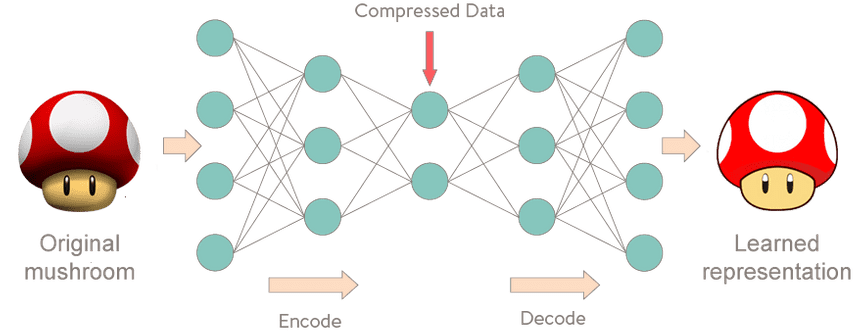
\includegraphics[scale=0.4]{mushroom_encoder}
							\caption{Exemplu de arhitectură auto-encoder. În partea stângă se poate observa imaginea inițială iar în partea dreaptă varianta compresata a acesteia obținută prin aplicarea auto-encoder-ului.}
							\label{fig:ae}							
						\end{figure}		
						O altă tehnică este folosirea unor tipuri de rețele neuronale specifice, folosite pentru procesarea datelor de intrare sau chiar crearea unora noi. Aceste rețele neuronale sunt numite \textit{autoencoders}. Autoenecoder-ele sunt alcătuite din minim trei nivele. Diferența față de rețele neuronale apare în faptul că dimensiunea intrărilor și ieșirilor este egală, în timp ce nivelele "ascunse", din interiorul rețelei, au dimensiuni mai mici. Astfel autoencoder-ele sunt altacuite din două părți: "encoder" și "decoder". Encoder-ul compreseaza datele cu scopul de a obține o varianta cât mai eficientă în care informațiile principale sunt încă păstrate. În schimb, decoder-ul are ca scop aducerea acestei forme compresate la o formă cât mai apropriată de cea inițială. Datele care trec prin această rețea sunt filtrate pentru a păstra doar informația complet necesară, Fig.\ref{fig:ae}. Prin modificări ușoare în arthitectura se pot obține funcționalități complet noi, ca de exemplu "Denoising Autoencoders" (DAE), care după aplicarea unui zgomot la datele de intrare au ca scop să determine ponderile necesare pentru extragerea acelui zgomot și readucerea intrărilor la o formă cât mai apropiată de cea "curată". În SER mai multe tipuri de autoencoder-e au fost folosite în încercarea de a mări acuratețea sistemului: Denoising Autoencoders (DAE) Chao et al., 2014 \cite{dae}, Adaptive Denoising Autoencoders (ADAE) Deng et al., 2014 \cite{adae}, sparse autoencoder (SAE) Deng et al., 2013 \cite{sdae}, adversarial autoencoder (AAE). \par
						Alte tehnici folosite sunt: 
						\begin{itemize}
							\setlength\topsep{0pt}
							\setlength\itemsep{0pt}
							\setlength{\itemindent}{1cm}
							\item "Multitask Learning", unde din cauza similitudinii dintre anumie sarcini părți dintr-un clasificator pot fi antrenate pe mai multe sarcini mărind astfel generalitatea modelului.
							\item "Transfer Learning", Prin această tehnică s-a încercat depășirea dezavantajului legat de lipsa bazelor de date suficiente. Astel diferite implementări se folsoesc de părți din alte modele care au fost pre-antrenate pe probleme similare ca "Speech Recognition" înainte de a începe antrenarea modelului pe cele specifice SER.
							\item "Voice Detection", Acest algoritm este folsoit pentru exluderea segmentelor care nu conțin vocea umană, pentru a reduce posibilele erori aduse de zonele lipsite de informație emoțională. 					
					\end{itemize}
				
				
				\section{Prezentarea unor implementări din SER} \label{papers}
					Cum am menționat și în capitolul precedent, "Speech Emotion Recognition" nu a ajuns în punctul în care poate fi pus pe piață, astfel am decis să fac o comparație teoretică incercând să prezint alte moduri de implementare prezente în câteva articole de cercetare. În continuare voi prezenta trei arhitecturi de sisteme din recunoașterea a emoției în vorbire, care susțin câteva din principalele idei pe care și eu mi-am bazat modelul. Deși prezintă unele similarități, acestea nu pot fi comparate in mod perfect deoarece folosesc atât baze de date diferite cât și caracteristici de intrare diferite. Deoarece nu există un mod consacrat de a construi un model SER, avantajele și dezavantajele dintre diferitele implementări devin dificil de identificat. \par		
					
					\subsection{A Cross-corpus Study on Speech Emotion Recognition} \label{prez_multi_domain}
					
					
					Milner et al.(2019) în articolul de cercetare "A Cross-corpus Study on Speech Emotion Recognition" \cite{multi-domain} folosesc un model antrenat pe mai multe baze de date constituite din înregistrări în aceiași limbă, Engleză, cu voci de aceeași vârstă, adulți. Acest articol încearcă să determine beneficiile folosirii  unor emoții jucate de actori profesioniști în combinație cu unele naturale. Cu atât mai mult, studiul iși propune să prezinte și avantajele folosirii conceptului de "multi-task learning" unde părți din același model sunt antrenate pe diferite sarcini asemănătoare pentru a mării eficiența antrenării pe același set de date de intrare. \par
					
					Arhitectură implementării propuse în Milner et al., 2019 \cite{multi-domain} implică folosirea unui set de caracteristici de intrare "hand-crafted" generate prin extragerea coeficienților MFCC, PLP ("perceptual linear prediction") și COVAREP \cite{covarep} din înregistrările audio. Modulul clasificator al arhitecturii este extrem de asemănător cu cel folosit de mine în acest proiect fiind constituit din două nivele de celule recurente LSTM bidirecționale  urmate de un mecanism de atenție, detaliate în \ref{RNN} respectiv \ref{attention}. Setul de emoții clasificate este alcătuit din: fericire, tristețe, enervare, surprindere, dezgust, frică și neutru. \par
					
					"Cross-corpus" se referă la antrenarea modelului folosind pe rând câte una din bazele de date dintr-un set și apoi testarea pe fiecare din cele rămase. "Multi-domain" înseamnă antrenare pe toate bazele de date și apoi testare pe anumie părți din fiecare. Motivele principale pentru care aceaste tehnici sunt folosite în practică sunt mărirea generalității modelului și combatrea numărului scăzut de înregistrări per baza de date. \par
					
					În acest articol s-au obținut rezultate foarte bune pentru ambele metode de utilizarea a bazelor de date, acuratețe ne-ponderată de  81.94\% în cazul "cross-corpus" și 82\% în cazul multi-domain. \par					
					
					Antrenarea "Multi-domain" nu a fost totuși cea mai de succes metodă folosită în acest articol de cercetarea. Milner et al., 2019 \cite{multi-domain} propun și folisrea tehnicii numite "domain adversarial training", unde pe lângă sarcina clasificării emoției, o parte din model a fost antrenată să recunoască și baza de date din care o înregistrarea face parte. Acest mecanism funcționează ca un regularizator în procesul de calcularea a erorii, fiind adunat la eroarea rezultată din sarcina principală, SER. Prin introducerea acestei îmbunătățiri acuratețea modelului crește atingând, 82.26\%. \par
						
					\subsection{Improved End-to-End Speech Emotion Recognition Using Self Attention	Mechanism and Multitask Learning} \label{end-to-end2}
					
					Li, Yuanchao et al., 2019 \cite{yuan} au reușit să obțină o acuratețea neponderată cu 14.3\% mai mare față de soluțiile tradionale prin metodă propusă. Aceată metodă se bazează pe conceptul de modele "end-to-end". Totuși arhitectura propusă se folosește și de alte tehnici ca mecanismul de atenție și antrenare "multi-task" pentru a depăși unele obstacole în recunoașterea emoțiilor în vorbire. \par
					
					Tehnica de extragere a caracteristicilor de intrare printr-un algoritm "machine learning" face ca toate modulele de procesare din interiorul modelului să fie antrenabile. De aici apare și numele tehnicii, "end-to-end". Aceste modele sunt extrem de avantajoase în SER, obținând rezultate încurajatoare \cite{adieu,e2e}. Folosirea unei astfel de extragere "automată" a caracteristicilor semnalelor reduce influența umană implicată în crearea modelului, deoarece nu mai necesită părerea unor specialiști în domeniul audio pentru a determina cele mai eficente caracteristici de intrare. Avantajele folosirii tehnicii "end-to-end" find descrise mai în detaliu atât în \ref{dif_fex} cât și în \ref{end-to-end}. \par
					
					Asemănător cu soluția propusă în Milner et al., 2019 \cite{multi-domain}, arhitectura folosește două nivele recurente bidirectionale la care s-a atașat un nivel de atenție și tehnica de  învățare "multi-task". Cu toate acestea, cea de a două sarcină pe care o execută clasificatorul nu mai este recunoașterea bazei de date ci a sexului persoanei care vorbește în înregistrare. Prin folosirea acestui tip de antrenare clasificatorul are posibiltatea să învețe diferențele între caracteristicile vocii unui vorbitor masculin și feminin. \par
					
					Modelul prezentat în acest articol stintific folosește o singură bază de date de intrare. Astfel modelul devine specializat în a recunoaște emoții pe acel set de date, dar va da un randament mai slab în inferență pe înregistrări din afara acestui set. Mulțimea de emoții clasificate este mai redusă  decât în cazul precedent, fiind constituită din emoțiile fericire, tristețe, enervare, și neutru, obțînând o acuratețe de 82.8\%, care depasete precizia de 68.5\% înregistrată folosind metodele precedente pe aceași bază de date.
					\subsection{Automatic speech emotion recognition using recurrent neural networks with local attention}
					 \label{prez_misramadi}
					 Misramadi et al. (2017) se focusează în articolul \cite{misramadi} pe evidențierea avantajului folosirii unei rețele neruonale recurente urmate de un nivel de atenție pentru studiul recunoașterii de emoțîi în vorbire. Succesul folosirii rețelelor recurente în domeniul SER a fost înregistrat în diferite soluții de-a lunglul anilor \cite{yuan,multi-domain,rnn1,rnn2}. Aceste rezultate prezintă cum folosirea unor rețele recurente profunde face ca modelul să învețe să recunoască atât informațiile emoționale de scurtă durată, per segment, cât și să extragă relațile temporale dintre acestea pe o perioada mai lungă de timp. \par
					 
					 \par 
					 Pe lângă folosirea acestor rețele neuronale ca modul principal de clasificare, in Misramadi et al. (2017) se propune folosirea unui mecanism de atenție bazat pe o sumă ponderată (prezentat în \ref{attention}). Ponderile acestui mecanism sunt la rândul lor antrenate în procesul de învățare. În acest articol, tehnica de atenție este propusă că o îmbunătățire la arhiecturile tradiționale ale sitemelor SER bazate pe rețele recurente. Beneficile aduse de acest mecanism sunt comparate cu alte modalități, mai puțîn de succes, de combinare a emoțiilor din segmentele semnalului audio pentru a obține informația emoționale totală pe intreagă înregistrare. \par
					 
					 Celelalte modalități care realizează această sarcină sunt, simpla recunoaștere a emoției în fiecare segment, folosirea informației emoționale doar din ultimul segment și realizarea mediei informațiilor emoționale din toate segmentele. Aceste tehnici prezintă un număr de dezavantaje care sublinează importanța folosirii unui mecanism de atenție ponderat. În primul rând, nu este rezonabil să asumăm că fiecare segment din înregistrarea audio conține informație emoțională. Deoarece pauzele în vorbire și zgomotul de fundal au o frecvența mare în majoritatea înregistrărilor, modelul ar trebui să fie cababil să filtreze aceste segmente care pot să îi dăuneze acurateții acestuia. Pe lângă asta, asumarea că ultimul segment conține informația emoțională totală a semnalului audio este falsă deoarece dacă informația emoțională principală se află la începutul propoziției (de exemplu un râset în prima secundă și apoi linișite până la finalul înregistrării) modelul va devia de la emoția recunoscută atunci din cauza influențelor celorlalte segmente care se suprapun peste informația emoțională inițială. Utilizarea operației de medie asupra întregului set de segmente nu este nici ea eficientă, deoarece segmentele lipsite deemoții vor continua să aibe un efect asupra clasificării. \par
					 
					 Din aceste motive, Misramadi et al., 2017 \cite{misramadi} propun folosirea unei sume ponderate, ponderile fiind invățate la antrenare, care va reuși să determine segmentele bogate în emoțîi și să își îndrepte atenția doar asupra acestora. 					 
					 Soluția prezentată în acest articol folosește o singură bază de date, extragerea datelor caracteristicilor este "hand-crafted", clasificatorul este alcătuit din două nivele recurente BLSTM (\ref{RNN}), iar setul de emoții clasificate este același cu cel folosit și în secțiunea precedentă: fericire, tristețe, enervare și neutru. Rezultatele obținute în acest studiu depășesc cu 3.1\% acuratețea neponderată obținută în soluțiile SER tradiționale bazate pe alt tip de clasificator, SVM ("Support Vector Machine").
					 
				\section{Prezentarea soluției propuse} \label{solutie}
					Considerând diferitele obstacole ale domeniului recunoașterii emoției în vorbire enumerate în sub-capitolul \ref{obstacole} și arhitecturile descrise în secțiunea anterioară, soluția pe care o propun în această lucrare de diplomă pentru recunoașterea emoției în vorbire este ilustrată în Fig \ref{fig:model}. \par
					Soluția SER propusă conține două module arhitecturale principale aferente extragerii caracteristicilor de intrare și construirii modelului clasificator. În continuare vor fi descrise pe scurt componentele care alcătuiesc aceste module, urmând să fie detaliate teoretic și practic în capitolele următoare. \par
						
					
					\begin{figure}[h]
						\noindent
						\hspace*{-1cm}
						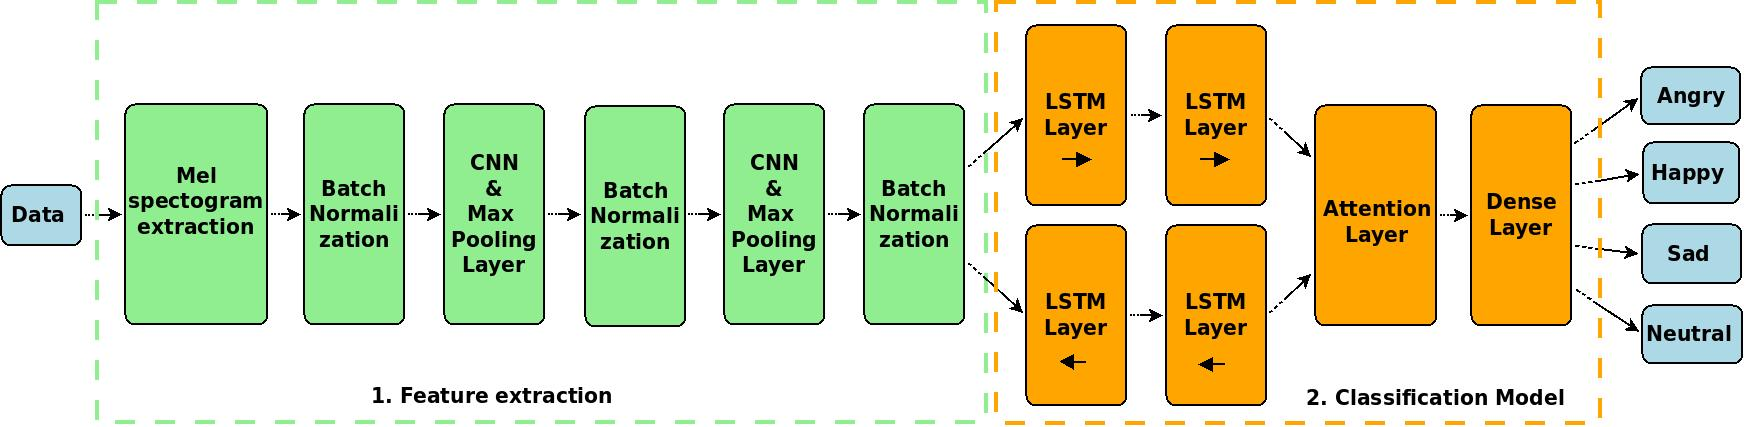
\includegraphics[scale=0.290]{Sistem_Diagram}
						\caption{Arhitectura propusă pentru sistemul de recunoaștere a emoțiilor, alcătuită din cele două etape principale: extragerea caracteristicilor de intrare din semnalul audio (verde) și modelul clasificator. (portocaliu).}\stepcounter{Figcount}
						\label{fig:model}
						
					\end{figure}
				
					Datele de intrare folosite în această lucrare provin dintr-un set de mai multe baze de date alcătuit din: 'EMO-DB', 'RAVDESS', 'EMOVO', 'MAV', 'ENTERFACE' și 'JL'. Similar cu motivația prezentată la \ref{prez_multi_domain}, decizia folosirii unui număr ridicat de baze de date este bazată pe depășirea dezavantajului numărului scăzut de exemple pentru antrenare specific domeniului SER, detaliată în 1.3.1. Deoarece semnalele audio sunt înregistrate în locații și limbi diferite, generalitatea modelului crește considerabil și face posibilă inferența pe înregistrări din afara acestor seturi de date. \par
					
					Extragerea caracteristicilor de intrare din semnalul audio este realizată atât în manieră "end-to-end" folosind o rețea neuronală convolutionala, \ref{cnns} cât și în manieră "hand-crafted" folosind operații matematice predefinite, \ref{hand-crafted}. Arhitectura propusă, Fig. \ref{fig:model}, folosește extragerea "end-to-end" iar metodă "hand-crafted" este folosită doar ca un termen de comparație și este prezentă doar în modul de utilizare pentru antrenare. Această decize este bazată pe rezultatele promițătoare obținute prin folosirea arhitecturilor "end-to-end"  în mai multe sisteme SER și pentru că, după cum am menționat anterior, nu s-a descoperit încă un set de caracteristici "hand-crafted" care să cuprindă perfect informația emoțională. Între fiecare nivel ale rețelei convoluționale am introdus tehnica numită "batch-normalization", \ref{batch-norn}, pentru a reduce fenomenul de expolize al gradienților și a grăbi procesul de antrenare. \par
					Structura internă a modulului clasificator ales a fost bazată pe raționamentul detaliat în Misramadi et al., 2017 \cite{misramadi}. Astfel, modelul clasificator este unul complex altcatuit din 3 componente: rețeaua recurentă, mecanismul de atenție și rețeaua neuronală densă, după cum se poate observă și în Fig. \ref{fig:model}.  
					Rețeaua neuronală recurentă este consituita din două celule recurente BLSTM ("Bidirectional Long Short-Term Memory") pe două nivele. Această tipologie de rețea neuronală a fost aleasă pentru a profita de relațiile temporale ale informațiillor emoționale dintre segmentele audio aflate la momente diferite. Rețeua recurentă este urmată de un mecanism de atenție care permite modelului să se focuseze doar pe segmentele semnalului audio bogate în emoție. Rețeaua neuronală generică densă este concatenată la modulul clasificator pentru a realiza translatarea rezultatelor rețelei recurente și a mecanismului de atenție în distribuția de probabilitate a emoțiilor clasificate.\par
					
					Numărul de emoții clasificate este patru, la fel că în arhitecturile din Misramadi et al., 2017 \cite{misramadi} și	Li, Yuanchao et al.2019 \cite{yuan}: fericire, tristețe, enervare și neutru. \par
					
					Lucrarea conține și o interfață grafică care permite utilizatorului să utilizeze sistemul de recunoaștere a emoțiilor în vorbire descris mai sus printr-o gamă largă de funcționalități. Interfața grafică permite două moduri de utilizare: antrenare și inferență. În partea de antrenare, utilizatorul poate să modifice configurația parametrilor modelului și să observe diferite statistici legate de starea acestuia în timpul procesului de învățare. În modul de utilizare inferențial, utilizatorul poate să clasifice emoțiile din fișiere audio pre-înregistrate sau din semnale înregistrate pe loc prin intermediul interfeței grafice.\par			
							
			\chapter{Bazele teoretice}				 
				 Domeniul inteligenței artificiale diferă de oricare altă ramură a științei calculatoarelor deoarece își propune să rezolve problemele printr-o manieră stohastică. Avantajul privirii problemelor într-un mod probabilistic este că ne permite să aplicăm alogritmii obtinuiti direct în lumea reală. Algoritmii clasici pot fi extrem de performanți când vine vorba de a găsii soluțîi în timp polinomial, dar neputincioși dacă problema necesită soluții de un grad mai înalt de complexitate, timp exponențial. Lumea în care trăim este plină de astfel de probleme, iar abordările clasice funcționează doar pe difeirte abstractizări în care aspectele stohastice sunt eliminate aproape complet. \par				 
				 Metodă propusă de domeniul inteligenței artificiale este de a înlocui abordarea tradițională în care programatorul dictează pașii care duc la rezolvarea problemei cu un proces de antrenare prin care algorimtului ii sunt oferite doar un set de unelte pe care trebuie să învețe să le folosească singur din greșeli. \par			 
				 Recunoașterea emoțiilor în vorbire face parte din mulțimea acestor probleme denumite "grele", putând deveni o sarcină dificilă chiar și pentru oameni. Rezolvarea unei astfel de probleme poate fi realizată doar prin folosirea unei arhitecturi bazate pe inteligența artificială. Din acest motiv în urma studierii mai multor implementări prezentate în diferite articole stintifice din acest domeniu am decis să construiesc un model de clasificare cu arhitectură din Fig. \ref{fig:model}. \par
				 După cum se poate observă în figura de mai sus, sistemul SER propus este alcătuit din două părți principale: extragerea caracteristicilor de intrare și modelul clasificator. Fiecare din modulele care alcătuiesc aceste părți reprezintă decizii arhitecturale a căror motivație teoretică și practică uremaza să fie descrisă în secțiunile următoare. Deoarece extragerea caracteristicilor de intrare este realizată atât prin tehnica "hand-crafted" cât și "end-to-end", aspectele teoretice folosite de ambele metode vor fi descrise. Cu toate acestea, arhitectura propsa este cea "end-to-end", ilustrată în Fig. \ref{fig:model}.
			\section{Machine learning și rețele neuronale artificiale} \label{ml}
			"Machine Learning"-ul este domeniul de studiu care oferă calculatoarelor abilitatea de a învăța o sarcina fără să fie explicit programate pentru a face acest lucru. " [Arthur Samule, 1959]  \par
			
			Era în care ne aflăm este des numită "big dată era", sugerând cantinatea imensă de informații pe care omenirea o deține pentru prima dată în istorie. În același timp, tehnologia a evoluat până în punctul în care putem să creăm alogritmi care să se folosească de aceste informații pentru a rezolva sarcini care păreau până acum imposibil de rezolvat pentru algorimtii generici. "Machine Learning" este domeniul reprezentativ pentru acest tip de algoritmi, alcătuind un set de metode care pot detecta relațiile din interiorul datelor de intrare, și să se folosească de aceste relații învățate pentru a face predicții pe seturi de date noi. \par
			
			"Machine learning"-ul este structurat în patru mari tipuri de algoritmi: supervizați, nesupervizati, semi-supervizați și așa numiții "reinforcement learning algorithms". Proiectul meu este orientat pe găsirea unei soluții pentru recunoașterea emoției din vorbire. Această recunoaștere se numește în termeni tehnici \textit{clasificare}, și face parte din ramură algoritmilor supervizați pe care urmează să mă axez în continuare. \par 
			Algoritmii supervizați trebuie să facă o mapare de la un număr de întrări $X$ la un număr ieșiri $y$ după ce au procesat un set de perechi $D={(x_i,y_i)}^N_{i=1}$, numit set de date de antrenare. Algoritmii supervizați sunt ghidați astfel să găsească o soluție pentru o anumită problema printr-un set de exemple prin care li se prezintă un set de intrări și rezultatele dorite , conexiunea dintre intrare și ieșire rămânând să fie determinată de aceștia printr-un proces de învățare din greșeli. \par
			
			Termenul de "deep learning" se referă la o sub-diviziune a domeniului "Machine Learning", fiind specialzata pe folosirea rețelelor neuronale profunde. Aceste rețele neuronale sunt denumite profunde deoarece reprezintă un set de funcții, nivele, aranjate într-un lanț aciclic, Fig. \ref{fig:nns}. Primul nivel se numește de obicei nivelul de intrare , nivelele din interiorul acestui lanț se numesc "ascunse", iar nivelul de final se numește nivel de ieșire. După cum se poate observa în Fig. \ref{fig:nns} fiecare din nivele unei rețele neuronale este alcătuit la rândul lui dintr-un număr de neuroni. Arhitectura unei rețele neuronale este bazată pe conexiunile neuronale ale creierului, unde activarea unui neuron poate determina activarea unui alt neuron la care este conectat, obțînându-se astfel o reacție în lanț care are ca scop final realizarea unor procese complexe. 
			
			\begin{figure}[t]
			\centering
			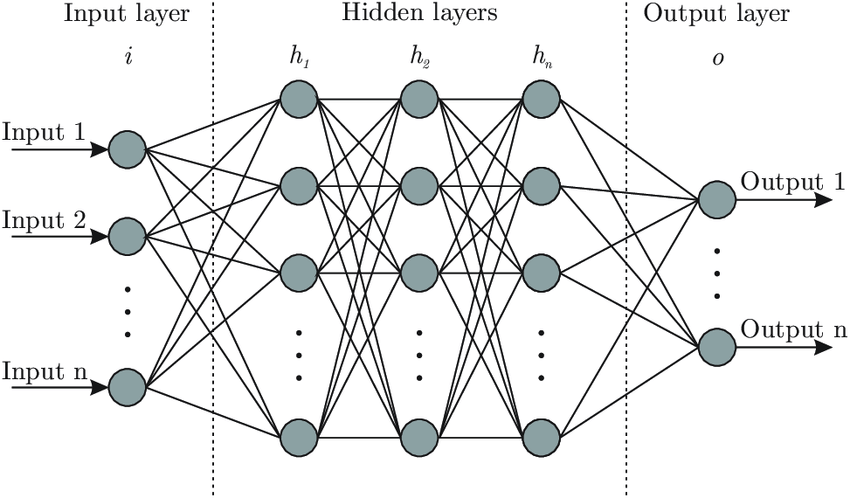
\includegraphics[scale=0.50]{nns}
			\caption{SStructura internă a unei rețele neuronale dense. Fiecare nod este conectat la toate nodurile din nivelele adiacente, iar între nivelul de intrare și ieșire există un număr arbitrar de nivele "ascunse". Figura aparține articolului Facundo et al. (2017) \cite{nnspic}}
			\label{fig:nns}
			\end{figure}	
			
			Neuronii unei rețele neuronale artificale generice sunt alcătuiți dintr-un set de ponderi care odată înmulțite cu fiecare intrare și adunate cu un coeficent, numit "bias", generează la rândul lor o intrare pentru neuronii umratori. 
			\noindent Ieșirea fiecărui neuron este determinată după formulă următoare:
			\begin{equation}
					a_j^{(i)} = \sum_{k=1}^{M} w_{jk}^{(i)} + w_{j0}^{(i)}
			\end{equation}
			
			unde $a_j^{(i)}$ reprezintă activarea neuronului $j$ din nivelul $i$, iar $w_{jk}^{(i)}$ și $w_{j0}^{(i)}$ reprezintă ponderile respective coeficientul "bias" al acelui neuron. \par
			
			Deși prin conectarea unor astfel de neuroni se pot obține arhitecturi complicate, pentru ca o rețea neuronală să se poată să aproximeze funcții complexe fiecare din ieșirile acestor neuroni trebuie să fie urmate de o așa numită \textit{funcție de activare}. Această funcție de activare are rolul de a elimina liniaritatea din interiorul rețelei neuronale și să mărească astfel numărul gradelor de libertate. Fiecare nivel poate fi reprezentat printr-o matrice iar fiecare trecere prin acel nivel poate fi exprimată printr-o înmulțire matricială. Fără existența acestor funcții de activare rețeaua neruonala ar fi doar un set de înmulțiri matriciale, care la rândul lui poate fi reprezentat ca o matrice unică, eliminând în sine sensul rețelelor adânci. Din acest motiv activarea unui neuron devine $h_j^{(i)} = z(a_j^{(i)})$, unde $z$ este funcția de activare aleasă. \par
			\noindent Unele dintre cele mai populare funcții de activare sunt:
			\begin{itemize}
				\item \textit{Sigmoid},  $f(x) = \frac{1}{1+e^{-x}}$, care aduce valoarea lui $x$ in intervalul (0, 1)
				\begin{figure}[h]
					\centering
					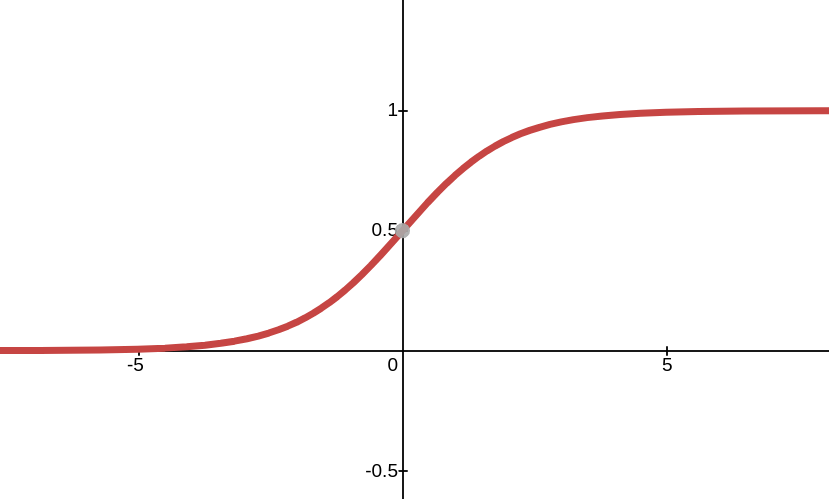
\includegraphics[scale=0.20]{sigmoid}
					\label{fig:sigmoid}
				\end{figure}
				\newline	
				\item \textit{Tangenta hiperbolică},  $f(x) = \frac{(e^x-e^{-x})}{(e^x+e^{-x})}$, care aduce valoarea lui $x$ in intervalul (-1, 1)
				\begin{figure}[!h]
					\centering
					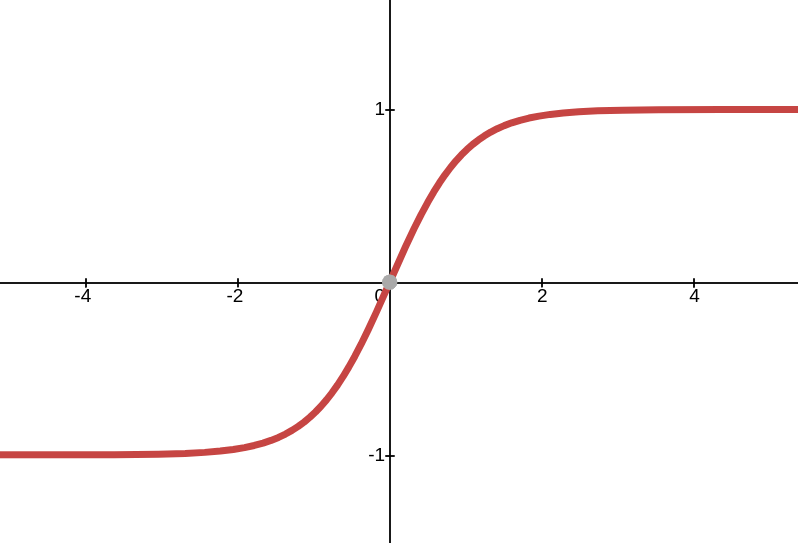
\includegraphics[scale=0.20]{tanh}
					\label{fig:tanh}
				\end{figure}	
				\item \textit{ReLu}, $f(x) = \max(0, x)$, care aduce valoarea lui $x$ in intervalul  [0, $\inf$)
				\begin{figure}[!h]
					\centering
					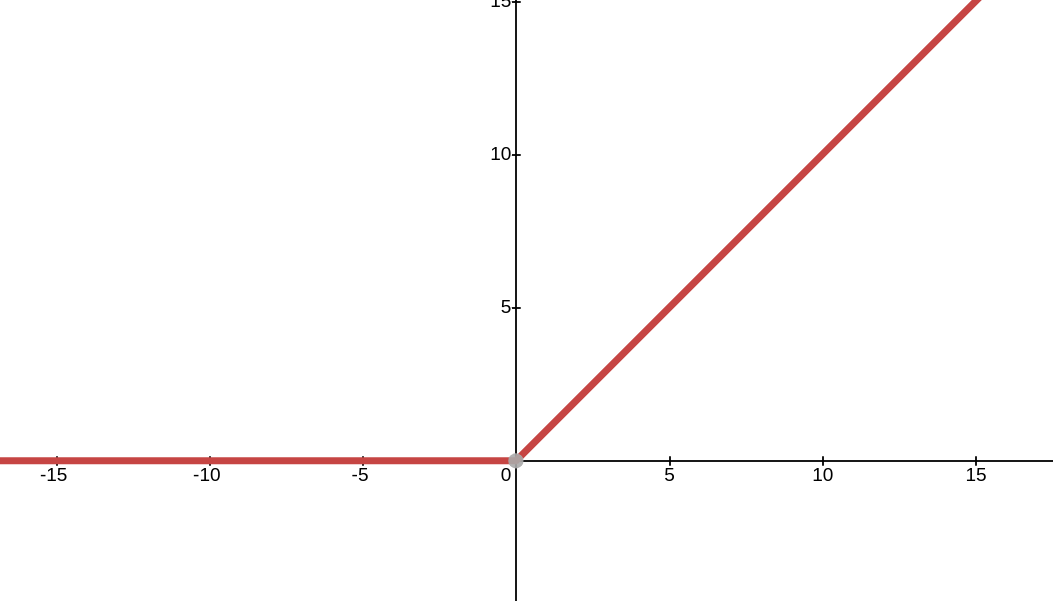
\includegraphics[scale=0.16]{relu}
					\label{fig:relu}
				\end{figure}	
				\item \textit{Leaky ReLu}, $f(x) = \max(0.01x, x)$, care aduce valoarea lui $x$ in intervalul  ($-\inf$, $\inf$)
				\begin{figure}[!h]
					\centering
					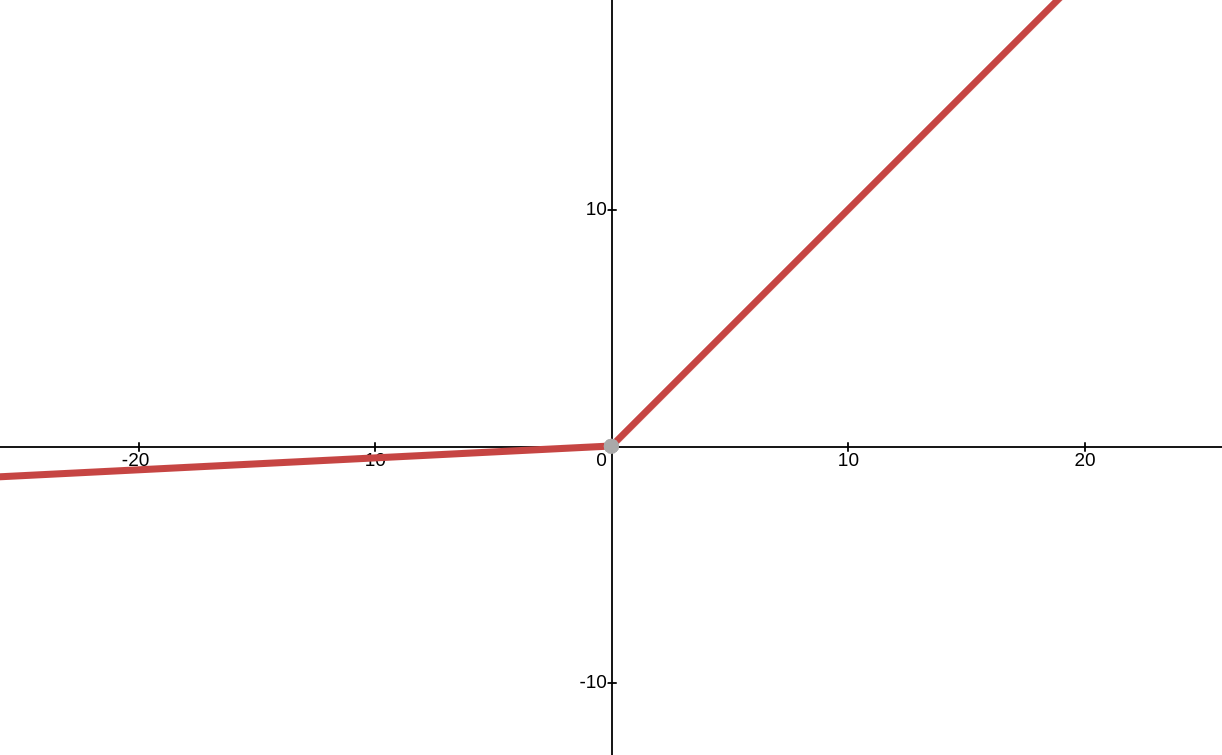
\includegraphics[scale=0.14]{lrelu}
					\label{fig:lrelu}
				\end{figure}
			\newpage
				\item \textit{ELu}, $f(x) = \max(\alpha (e^x -1), x)$, care aduce valoarea lui $x$ in intervalul ($-\inf$, $\inf$)
				\begin{figure}[!h]
					\centering
					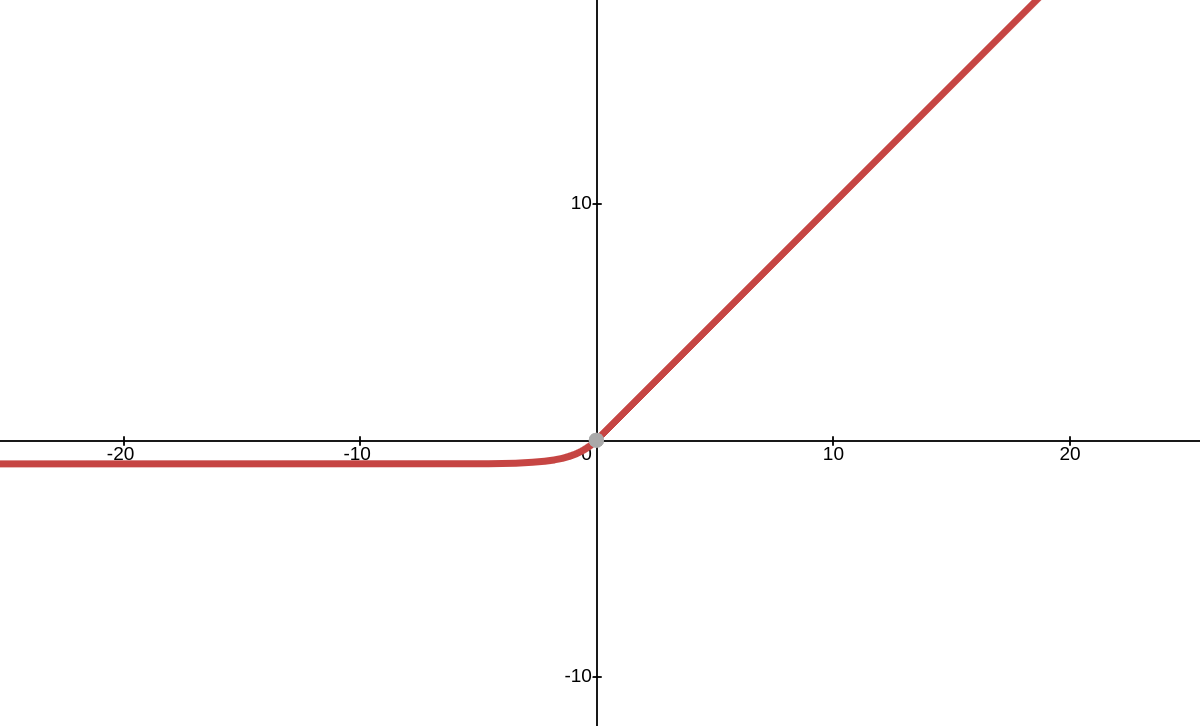
\includegraphics[scale=0.14]{elu}
					\label{fig:elu}
				\end{figure}	
			\end{itemize}
			\iffalse
			\begin{figure}[h]
				\begin{center}$
					\begin{array}{rr}
					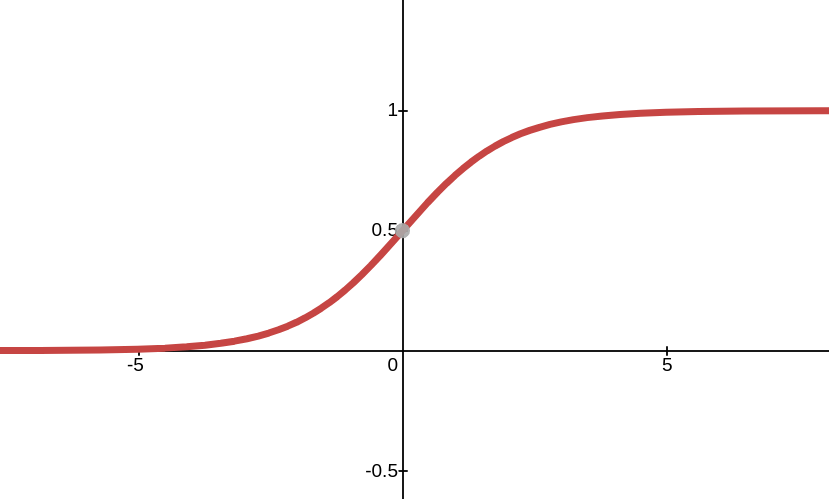
\includegraphics[scale=0.20]{sigmoid}&
					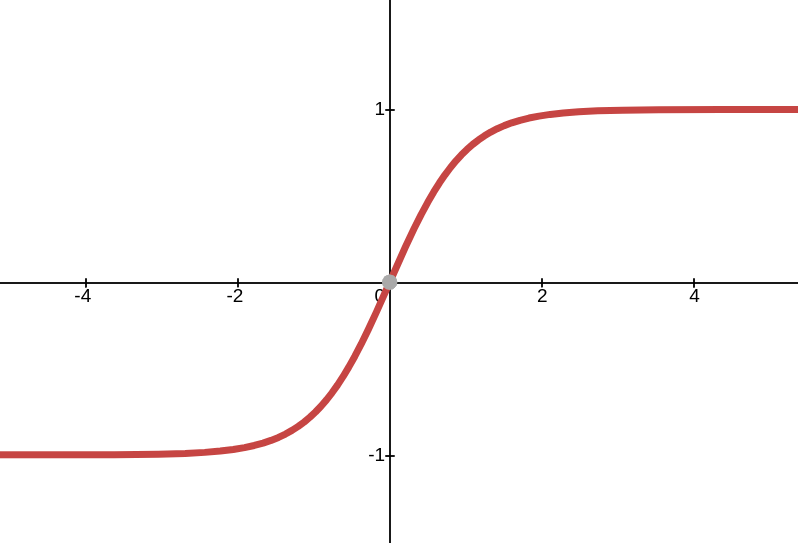
\includegraphics[scale=0.20]{tanh}
					\end{array}$
				\end{center}
				
				\begin{center}$
					\begin{array}{rr}
					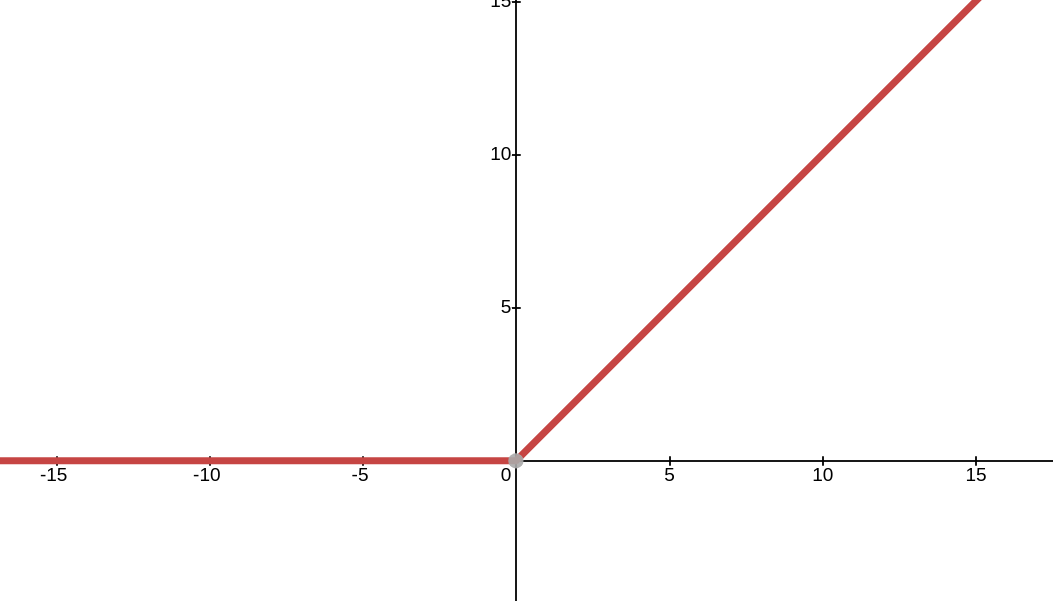
\includegraphics[scale=0.16]{relu}&
					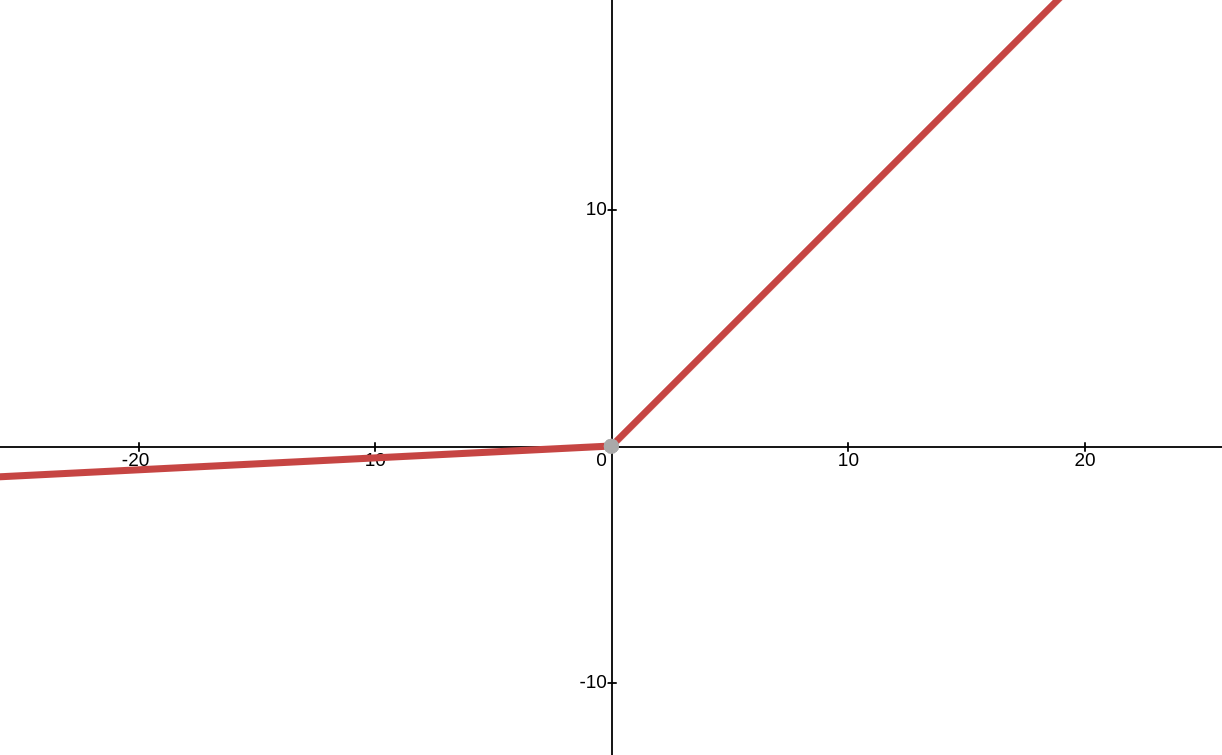
\includegraphics[scale=0.14]{lrelu}
					\end{array}$
					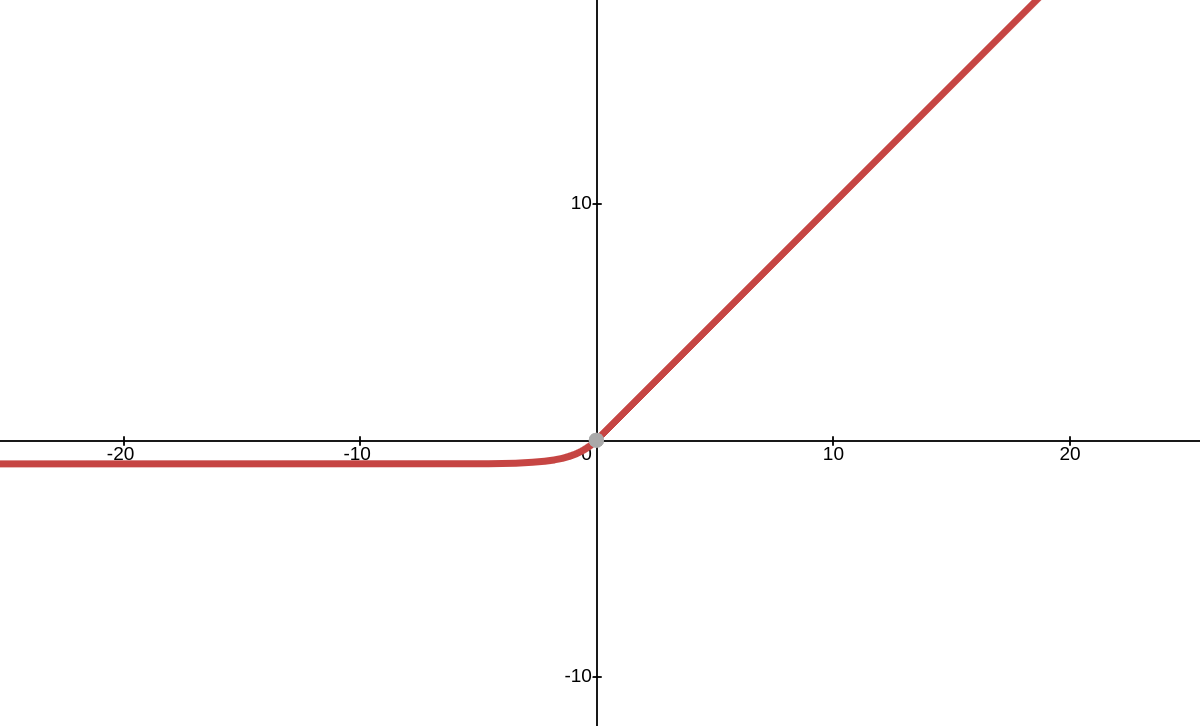
\includegraphics[scale=0.14]{elu}
				\end{center}
				\caption{Figure caption}
				\label{pics:blablabla}
			\end{figure}
			\fi
			În funcție de problem pe care dorim să o rezolvăm, nivelul de ieșire poate să conțînă la rândul lui o astfel de funcție de activare. În cazul clasificării binare este folosită funcția sigmoid iar în cazul clasifiarii unui număr mai mare de clase de obicei se folosește funcția "cross-entropy". Pentru regresie, sau alte probleme care nu clasifică datele de intrare, nivelul final nu este urmat de o astfel de funcție. \par
			
			Antrenarea rețelelor neuronale se realizează prin folosirea unor algoritmi numiți optimizatori. Aceștia determină influența pe care fiecare pondere din rețea a avut-o asupra rezultatului final extrăgând derivata ponderii în raport cu eroare totală a rețelei. Dacă acea influență a fost mare ponderea este modificată puternic, în caz contrar aceasta este modificat puțin. Prin folosirea unui număr mare de astfel de exemple ponderile ajung să conveargă la un set de valori care permit aproximarea unei multitudini de funcții complexe. \par
			
			Funcția de calcul a erorii poate avea forme diferite, dar una din cele mai folosite este eroarea pătrătica medie \ref{rms}.
			\begin{equation} \label{rms}
				E(W) = \frac{1}{2} \sum_{n=1}^{N} (y(x_n, W) - t_n)^2
			\end{equation}
			unde $E(W)$ este eroarea calculată, $N$ reprezintă numărul total de exemple de antrenare, $y(x_n, W)$ este predicia pentru exemplul cu numărul $n$ iar $t_n$ este valoarea adevărată. \par
			
			Recunoașterea emoției în vorbire este o problemă de clasificare. În acest caz, $y(x_n, W)$ reprezintă o distribuție de probabilitate asupra emoțiilor estimate de model iar $t_n$ este un vector de forma $[0,1,0,0]$, în care valoarea $1$ este pe poziția emoției aferente acelui exemplu. \par
			
			În arhitectura acestui proiect am folosit mai multe tipuri de rețele neuronale pentru îndeplinirea mai multor funcționalități. Aceste tipologii și modul lor de utilizare urmează să fie descrise în detaliu în sub-capitolele următoare.
			\section{Transformata Fourier discretă} 
			
			Orice formă de undă, indiferent dacă e observată în univers sau mâzgălită de noi pe foaie, reprezintă de fapt doar o sumă de funcții sinusoidale de diferite frecvențe.\par
			
			Un semnal audio este un semnal complex alcătuit din mai multe unde de diferite frecvențe care circulă sub formă unor perturbații prin mediu. Atunci când înregistrăm un semnal audio capturăm doar amplitudinile rezultate în urma combinării acestor unde. Transformata Fourier este un concept matematic care ne permite să descompunem un semnal în frecvențele care îl compun și magnitudinile acestora.\par 
			
			Motivul folosirii transformatei Fourier vine de la studiul seriilor Fourier. Prin studiul acestor serii, funcții periodice complicate sunt scrise ca simple sume de unde reprezentate matematic prin funcțiile sinus și cosinus.\par
			
			Fie o funcție periodică $f(t)$, cu o perioada fundamentală $T$, aceasta are aferentă seria Fourier următoare:
			\begin{equation}
				g(t) = a_0 + \sum_{m=1}^{\infty} a_m \cos(\frac{2\pi m t}{T}) + \sum_{n=1}^{\infty} b_n \sin(\frac{2\pi n t}{T})
			\end{equation}			
			unde $a_0$, $a_m$ si $b_n$ sunt coeficienții Fourier calculați sub forma			 
			\begin{align}
			\nonumber 	a_0 &= \frac{1}{T} \int_{0}^{T} f(t) dt\\
			\nonumber 	a_m &= \frac{2}{T} \int_{0}^{T} f(t) \cos(\frac{2 \pi m t}{T}) dt \\ 
						b_n &= \frac{2}{T} \int_{0}^{T} f(t) \sin(\frac{2 \pi n t}{T}) dt \label{coef_fr}
			\end{align}
			Aceste relații pot fi scrise într-o formă mai elegantă din punct de vedere matematic prin folosirea numerelor complexe, și mai exact a formulei lui Euler, \(\mathrm{e}^{2\pi i\theta} = \cos (2\pi \theta) + i \sin (2\pi \theta)\).			
			\begin{equation} \label{cmpl_frs}
				g(t) = \sum_{n=-\infty}^{\infty} c_n  \mathrm{e}^{i \frac{2\pi n t}{T}} 
			\end{equation}
			unde $c_n$ reprezintă echivalentul coeficientiilor Fourier $a_m$ și $b_n$ din \ref{coef_fr}			
			\begin{equation*}
			 	c_n = \frac{1}{T} \int_{0}^{T} f(t) \mathrm{e}^{-i \frac{2\pi n t}{T}} dt
			\end{equation*}
			
			Transformata Fourier este o operație care se aplică unei funcții complexe și produce o altă funcție complexă care conține aceeași informație ca funcția originală, dar reorganizată după frecvențele componente. Transforamta Fourier este o generalizare a seriilor Fourier complexe prezentate în \ref{cmpl_frs}, putând fi văzută că limita seriei Fourier când perioada tinde la infinit.
			
			Fie $f : R \to C$ absolut integrabilă. Funcția complexă de variabilă reală	$F : R \to C$,
			\begin{equation*}
						F(\omega) = \int_{-\infty}^{\infty}  \mathrm{e}^{-2\pi i\omega t} f(t) dt
			\end{equation*}
				se numește transformată Fourier a funcției f, iar
			
			\begin{equation*}
				f(t) = \int_{-\infty}^{\infty}  \mathrm{e}^{2\pi i\omega t} F(\omega) d\alpha
			\end{equation*}
			se nu meste inversa tranformatei Fourier. \par
			Astfel transformata Fourier reprezintă o unealtă care ne permite să schimbăm unghiul din care privim diferitele semnale de tip undă, făcând posibilă trecerea din domeniul temporal în domeniul frecvență Fig.\ref{fig:tf}. Acest domeniu ne permite să diferențiem între semnalele de diferite frecvențe care alcătuiesc unda. Prin folosirea inversei transformatei Fourier, putem chiar să eliminăm anumite semnale prin modificarea coeficientiilor aferenți frecvențelor acestora. Acest concept a deschis granitile unei arii uriașe de aplicații ale acestei teoreme, fiind revoluționară pentru domeniul procesării semnalelor.  	
				\begin{figure}[h]
					\centering
					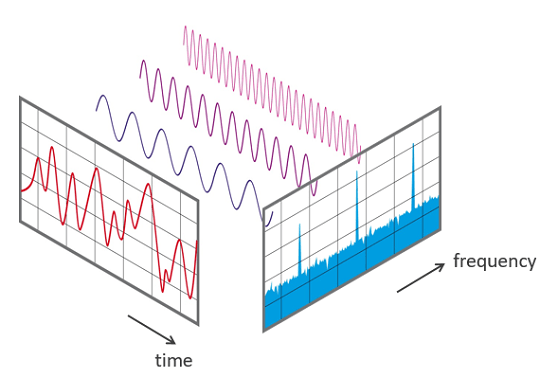
\includegraphics[scale=0.50]{ft}
					\caption{Ilustrare grafică a translatării semnalului audio în domeniul frecvență după aplicarea transformatei Fourier. Figura aparține paginii web din Trekhleb, 2018 \cite{stft6}.}
					\label{fig:tf}
				\end{figure}		
				
			"Short-time Fourier transform", sau STFT, este o varianta a transformatei Fourier prezentată mai sus, folosită pentru a determina frecventele sinusoidale și magnitudinile unor secțiuni locale dintr-un semnal. În practică, procedura prin care se calculează funcțiile STFT este de a împărții semnalul temporal în segmente mai mici de dimensiuni egale și apoi de a calcula transformată Fourier pe fiecare din aceste segmente separat. 
			\begin{equation*}
			STFT(r , \omega) = \int_{-\infty}^{\infty}  f(t) w(t-r)\mathrm{e}^{- i 2\pi \omega t}  dt
			\end{equation*}
			unde w(r) este o funcție fereastră. \par
			STFT oferă informații asupra frecvenței pe un anumit interval temporal local, fiind folosită în situații în care frecventele componente ale unui semnal variază puternic în timp. Transformata Fourier în schimb oferă doar media informațiilor frecvențelor pe întregul interval de timp al semnalului \cite{stft2}.
			
			Deoarece semnalul audio este discretizat si segmentat, in procesarea acestuia se foloseste varianta discreta a STFT.
			
			\begin{equation}
			STFT(m ,\omega) = \sum_{n=-\infty}^{\infty}  f[n] w[n-m]\mathrm{e}^{- i 2\pi \omega n}  \label{stft}
			\end{equation}
			
			
			\section{Caracteristicile Hand-crafted} \label{hand-crafted}
			
			Metoda "hand-crafted" de extrage a caracteristicilor de intrare din semnalul audio este bazată pe diferite formule matematice. După cum am spus și în sub-capitolul 1.3, momentan nu există un set de caracteristici reprezentative pentru informația emoțională, iar majoritatea implementărilor aleg aceste caracteristici printr-o selecție empirică. Majoriatea caracteristicilor fiind importate din problema recunoașterii informației lingivstice din vorbire, "Speech Recognition". \par 
			Chiar dacă alegerea setului de caracteristici este subiectivă fiecărei implementări, majoritatea împărtășesc un set restrâns care se consideră că surprinde anumite informații din discursul uman. Coeficientii Mel cepstrali și functile delta și delta-delta ale acestora fac de obicei parte din datele de intrare a sistemelor SER "hand-crafted" și din cauza populariatii acestora urmează să le descriu în continuare. \par
			
			\subsection{Coeficientii Mel cepstrali}
				Coeficienții Mel cepstrali, sau MFCC, sunt cea mai folosită reprezentare a prorietatiilor spectrale ale semnalelor vocale. Aceștia funcționează cel mai bine în cazul domeniului "Speech Recognition" deoarece iau în calcul senzitivitatea percepției umane în interpretarea frecvențelor prezente în semnalul audio. Pentru calcularea acestor coeficienți, trebuie să urmăm o serie de pași \cite{mcs}.
					\begin{enumerate}
						\item 
							În primul rând se calculează o estimare a densității spectrale a semnalului, așa numite "Periodogram estimate of the power spectrum". Pentru calcularea acesteia se aplică transformata Fourier pe termen scurt \ref{stft} pe fiecare segment din semnalul audio. Odată obținut echivaletul semnalului audio în domeniul frecvența , numit "complex spectrum", se ridică la pătrat valoarea absolută a acesteia pentru obținerea "Periodogram"-ei.
							\begin{equation*}
								P_i(k) =\frac{1}{N}\mid STFT(i, k)\mid^2 \quad\quad,1\leq k\leq K
							\end{equation*}
							unde $i$ este numărul segmentului actual, $N$ este numărul total de segmente audio și $K$ este frecvența maximă, sau "lungimea transformatei Fourier discrete".
							\item Următorul pas este aplicarea așa-ziselor "Mel filerbanks". "Mel filerbanks" sunt filtre triunghiulare care au valori nule pe majoritatea lungimii spectrum-ului. Aceste filtre se calculează prin scalarea unor frecvențe alese la distanțe egale dintr-un interval, de obicei $[300Hz, 8000Hz]$, în scară Mel. Această scară reprezintă limitele capacității umane de percepere a diferitelor frecvente sonore. Scalarea frecvențelor se realizează prin formula $M(f) = 1125 \ln(1+ f/700)$. Oamenii sunt mult mai buni în a diferenția schimbări la frecvente mici față de frecvente înalte, iar prin încorporarea aceste scalări caracteristicile obținute vor fi mult mai apropiate de ce ar auzi defapt un om. \newline
							După ce s-a aplicat complet scalare Mel se crează filtrele triunghiulare folosint următoarea formula
						\begin{equation*}
							H_m(k) = 
							\begin{cases}
							\quad \quad 0&\quad k<f(m-1) \\[3pt]
							\frac{k-f(m-1)}{f(m) - f(m-1)}&\quad f(m-1)\leq k\leq f(m) \\[5pt]
							\frac{f(m+1)-k}{f(m+1) - f(m)}&\quad f(m)\leq k\leq f(m+1) \\[3pt]
							\quad \quad 0&\quad k>f(m+1)
							\end{cases}
						\end{equation*}
						unde $m$ este numărul frecvenței scalate, iar $k$ este frecvența curentă din spectrum. \newline
						Filtrele triunghiulare sunt înmulțite apoi cu "power spectrum"-ul obținut la pasul anterior și se obțin astfel energiile din fiecare filtru Mel.
						\item Următorul pas reprezintă logaritmarea acestor energi.
						\item Ultimul pas fiind aplicarea transformatei cosinus discretă (DCT). Motivația acestui pas este că energiile obținute anterior au un grad ridicat de corelație iar aplicarea DCT realizează decorelara lor și oferă reprezentarea compresată a acestora.
						Formula pentru DCT fiind,
						\begin{equation*}
							X_k = \frac{1}{2}(x_0 + (-1)^k x_{N-1}) + \sum_{n=1}^{N-2} x_n cos[\frac{\pi}{N-1}nk]
						\end{equation*}
						Amplitudinile spectrum-ului rezultat reprezintă coeficienții Mel cepstrali.
				\end{enumerate} \par
				\subsection{Deltas si delta-deltas}
					Totuși, coeficienții Mel descriu doar coperta puterii spectrale a fiecărui segment din semnalul audio, dar s-a demonstrat empiric că o parte importantă din informația vocală se află și în spatele dinamicii acestor coeficienți. Acest lucru se calculează folosind caracteristicile delta și delta-deltas. \par Coeficienții deltas sunt calculați din MFCC prin următoarea formulă:
					\begin{equation*}
						d_t = \frac{\sum_{n=1}^{N} n(c_{t+n}-c{t-n})}{2\sum_{n=1}^{N}n^2}
					\end{equation*}
					unde $d_t$ reprezintă coeficientul delta, din segmentul $t$  în funcție de coeficienții statici $c_{t+n}$ și $c_{t-n}$. 
					Coeficienții delta-delta sunt calculați prin aceeași formulă, înlocuindu-se doar coeficentii MFCC cu cei delta. \par
				
				Pe lângă acești coeficienți, caracteristicile "hand-crafted" pot conține și următoarele: tonalitate, probabilitate vocală, energie,  radicalul mediei amplitudinii la pătrat, rata zero-crossing, chroma, coeficientul rollof, rația harmonics-to-noise, bruiajul, media, variația, minimul și maximul semnalului audio etc. Toate acestea se calculează cu funcții matematice predefinite asemănătoare cu procesul de obținere a coeficentiilor MFCC.			
				
				În implementarea extragerii caracteristicilor "hand-crafted" folosită de mine am folosit: MFCC, delta, delta-deltas, radicalul mediei la pătrat a amplitudinii fiecărui segment, rata zero-crossing, chroma și coeficientul rollof.
				
			\section{Extragerea caracteristicilor End-to-end}	\label{end-to-end}
			
			Avansările recente ale algoritmilor și a hardware-ului calculatoarelor au făcut posibilă antrenarea rețelelor neuronale într-o manieră end-to-end pentru sarcini care necesitau în trecut expertiza umană. Pe lângă că aceste arhitecturi de rețele neuronale solicită mai puțin efort uman decât abordările tradiționale, în general acestea obțin și performanțe superioare. Acest aspect este în mod particular adevărat atunci când cantitatea de date pentru antrenare disponibilă este mare, deoarece beneficiile optimizării holistice tinde să  le depășească pe acelea a cunoștințelor anterioare  \cite{graves}. \par
			
			Arhitectura "end-to-end" este prezentată în Fig. \ref{fig:model}. După cum poate fi observat, extragerea caracteristicilor în această  arhitectură este realizată prin atașarea unei rețele convoluționale combinată cu o tehnică de normalizare între fiecare nivel. Aceste rețele convoluționale sunt celebre pentru procesarea imaginilor pentru că, spre deosebire de rețelele neuroanle artificiale normale, se folosesc de relațiile spațiale bidimensionale dintre pixeli. Astfel pentru a ne folosi de acest avantaj se extrage spectograma Mel a semnalului audio, care va fi folosită ca date de intrare pentru aceste rețele. Un exemplu al unei astfel de spectograme se poate observa în Fig. \ref{fig:melspec}. \par
						
			\begin{figure}[h]
				\centering
				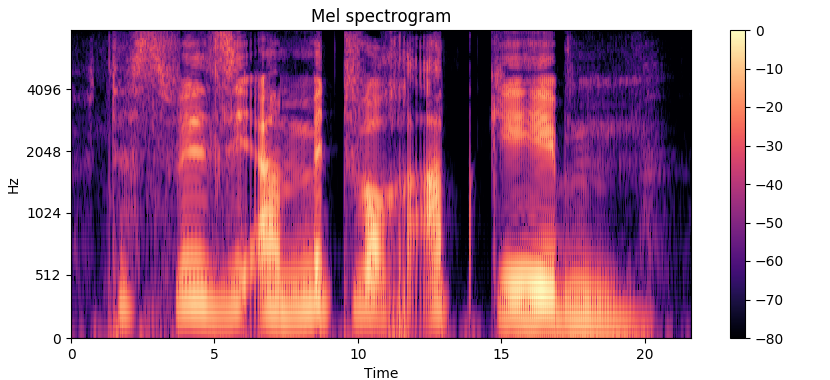
\includegraphics[scale=0.67]{melspectogram}
				\caption{Spectograma Mel a unui semnal audio extras cu ajutor librărie librosa \cite{librosa}. Spectograma ilustrează valoarea amplitudinilor frecventelor din fiecare moment al semnalului audio.}
				\label{fig:melspec}
			\end{figure}
			
			\subsection{Spectograma Mel} \label{mel}
				Prin spectograma se înțelege reprezentarea vizuală a unui spectrum de frecvențe a unui semnal în raport cu timpul. Astfel într-o spectogramă axa orizontală reprezintă timpul, axa verticală reprezintă frecvența iar intensitatea culorii reprezintă magnitudinrea(amplitudinea) frecvenței observate la acel moment din timp. Calcularea spectogrameleor Mel este extrem de asemănătoare cu calcularea coeficientilor de corelați Mel prezentați în sub-sub-capitolul 3.1.2. Astfel pașii 1, 2, și 3, prezentați anterior, se reproduc. Singura diferență este că în loc de calcularea transformatei cosinus discretă și extragerea coeficientilor ca la pasul 4, evoulutia valorile amplitudinii frecventelor în funcție de timp sunt translatate într-o matrice care va alcatuii spectograma. \par
			\subsection{Batch normalization} \label{batch-norn}
				Unul din motivele pentru care antrenarea rețelelor neuronale profunde, cu mai multe nivele, devine dificilă este faptul că distribuția intrărilor fiecărui nivel se schimbă în timpul antrenării, prin modificarea parametrilor nivelului anterior care le generează. Acest lucru încetinește drastic procesul de învățare al modelului deoarece alegerea modului de inițializare al parametrilor capătă un impact mult mai ridicat și face necesară alegerea unor rate de antrenare mai mici. Acest fenomen se numește "internal covariate shift", iar o soluție propusă de Ioffe \& Szegedy et al., 2015 \cite{batch_norm}, este normalizarea intrărilor fiecărui nivel. \par Formula pentru normalizare este cea generică:
				\begin{equation*}
					x'_i = \frac{x_i - \mu_B}{\sqrt{\sigma^2_B +  \varepsilon}}
				\end{equation*}
				
				\quad unde $x_i$ reprezintă intrarea cu numărul i, $\mu$ este media setului de intrări al nivelului curent, $\sigma$ este deviația standard a acestor intrări iar $\epsilon$ reprezintă doar o constanta pentru evitarea împărțirii la 0.
				
				Pe lângă reducerea fenomenului prezentat anterior, "internal covaraite shift", aceast mecanism de normalizare aduce alte două mari beneficii. În timpul antrenării gradienții circulă de la nivelul final al rețelei spre început modificând parametrii modelului pentru a reduce eroarea înregistrată.
				Prin folosirea normalizării înainte de fiecare nivel se reduce dependența acestor gradienți de scala ponderilor nivelelor rețelei și de valoarea lor inițială. Acest lucru ne permite să folosim rate de antrenare mai mari fără a pune în pericol convergența modelului. \par
				Cel de al doilea avantaj este că s-a demonstrat empiric \cite{batch_norm} că tehnica "batch normalization" îmbunătățește regularizarea parametrilor și mărirea generalității modelului. \par
				Modele SER sunt succeptibile la un fenomen denumit "explozia gradienților", deoarece folsoesc arhitecturi complexe cu un număr mare de parametrii. Pe lângă acest considerent, acuratețea acestor modele depinde puternic de variabile greu de controlat ca modul de înregistrare al bazelor de date, locația unde s-a desfășurat înregistrarea, multitudinea vorbitorilor, diferențele de exprimare și limbile folosite. "Batch normalizaton", oferă beneficii în ambele privințe deoarce funcționează că un regularizator, încetinind "exploziile" din interiorul nivelelor, și normalizează datele de intrare reducând astfel influența diferențelor de la o înregistrare la alta. \par
			\subsection{Rețele neurononale convoluționale} \label{cnns}
				Rețelele neuronale convoluționale, sau CNN, reprezintă o adaptare a rețelelor neuronale artificiale generice pentru rezolvarea sarcinilor vizuale, sau în care datele de intrare sunt organizate în două dimensiuni. Deși aceste tipuri de rețele neuronale au fost introduse prima dată în 1989 ((Le Cun et al., 1989 \cite{leCun}), au crescut în popularitate abia în ultimii ani, dominând astăzi majoritatea soluțiilor propuse pentru diferitele sarcini din domeniul vizual. \par 
				Conceptul principal din spatele acestor arhitecturi reprezintă operația matematică numită \textit{convoluție}, după care a și fost numită această tipologie de rețea neronala. Convoluția reprezitna o operație care primește ca intrări două funcții și reprezintă modul în care una dintre funcții își modifică forma în funcție de cea de a două funcție. Formula unei convolutii discrete este următoarea:
				\begin{equation*}
					s(t) = (f*g)(t) = \sum_{n=-\infty}^{\infty} f(n) \cdot g(t - n)
				\end{equation*}	\par
				\noindent sau in doua dimensiuni
				\begin{equation}\label{convo}				
					S(i, j) = (I*K)(i, j) = \sum_{m} \sum_{n} K(m, n) \cdot I(i - m, j - n)
				\end{equation}
				
				Bazată pe această formula matematică relativ simplă rețele neuronale convoluționale au reușit să depășească unele dintre principalele piedici pe care rețelele neuronale simple le întâlneau în procesarea imaginilor. Rețele neuronale tradiționale crează conexiuni între fiecare unitate de intrare și fiecare neuron din nivelul aferent. Având un număr satisfăcător de date de intrare acestea pot să învețe să rezolve diferite sarcini care par imposibile pentru alogiritmii generici din știința calculatoarelor. Totuși, dimensiuniea acestor arhitecturi poate crește extrem de rapid, iar pentru probleme ca procesarea imaginilor, unde diferite imagini pot avea sute de mii de pixeli, depășesc rapid capacitățile de procesare disponibile. \par
				Pe lângă acest dezavantaj, arhitecturile generice nu reușesc să suprindă esența procesării de imagini, sau a mecanismului de vedere uman, care este bazat pe conceptul că pixelii care se află în vecinataea unui anumit pixel sunt mult mai puternic corelați cu aceștia decât oricare alți pixeli. Astfel deși aceste nivele din rețelele neuronale generice se folosesc de întreaga informație de intrare rămân inflexibile când vine vorba de a determina anumite linii, curbe sau forme ale obiectelor observate, ele luând în considerare doar intensitatea culorii unui pixel dintr-o locație dată. \par
				
				Rețelele neuronale convoluționale reușesc să treacă peste aceste obstacole prin folosirea a trei idei care au adus multe beneficii și în alte tipologii de rețele neuronale,\textit{ filtre de recepție locale}, \textit{refolosirea parametriilor} și \textit{subesantionare}. \par
				
				Metodele tradiționale de antrenare folosesc înmulțirea matricială între întregul set de date de intrare și întregul set de parametrii dintr-un nivel. În schimb, CNN se folsoesc de așa numite \textit{filtre}, sau \textit{"kernels"}, care reprezintă un set de paramterii de dimensiuni de câteva ori mai mici decât datele de intrare. Aceste filtre sunt apoi înmulțite doar cu anumite parți echivalente dimensional din datele de intrare. Astfel, de exmplu având o imagine în dimensiuni 28x28 și un filtru de dimensiuni 3x3, acest filtru este aplicat pe bucăți de dimensiuni 3x3 din matricea intrărilor plimbandul pe întreagă suprafață a imaginii. Rezultatul obținut devine una din intrările unui filtru următor. Acest mecanism poate fi observat în Fig. \ref{fig:cnns}.
					
				\begin{figure}[h]
					\centering
					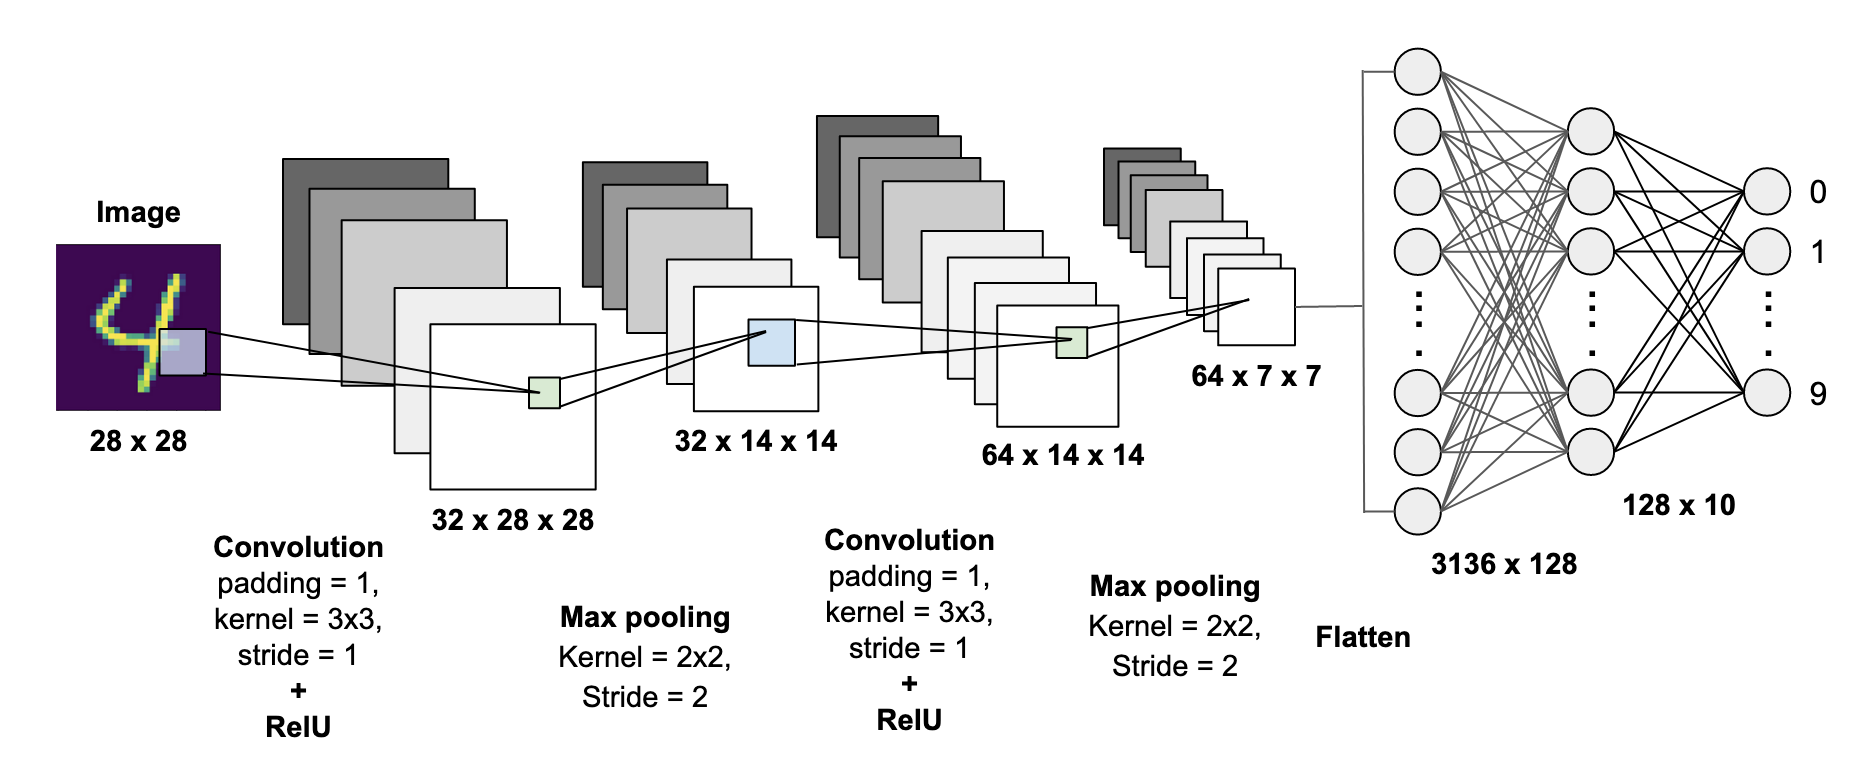
\includegraphics[scale=0.23]{cnns}
					\caption{Arhitectura unei rețele neuronale convoluționale specialziata pe recunoașterea cifrelor scrise de mâna. Figura aparține paginii din Patel, 2019 \cite{cnn_photo}}
					\label{fig:cnns}
				\end{figure}
				
				Simpla folosire a acestor filtre de dimensiuni reduse rezolva majoritatea problemlor impuse de arhitecturile tradiționale. În primul rând prin acest mod rețeaua neuronală primește capacitatea de a determina caracteristici abstracte. Acest lucru este posibil prin faptul că filtrele se focusează pe determinarea relațiilor din pixelii învecinați. În timpul antrenarii aceste filtre vor învață să detemine anumite caracteristici din interiorul imaginilor. Deoarece aceștia sunt aplicați succesiv pe intreagă imagine de intrare, ei o să determine existența și poziția acelor caracteristici oriunde în matricea de intrare. Nivelele de la baza rețelei învață să determine caracteristici simple că diferite puncte, linii sau curbe din diferite locații ale imaginii, în timp ce nivelele de la capătul rețelei prin combinarea informației de la filtrele anterioare ajung să determine carcateristici complexe, ca diferite forme sau obiecte. Operația de convoluie, \ref{convo}, prezintă perfect modul de aplicare al acestor filtre unde $I$ reprezintă imaginea iar $K$ filtrul aplicat pe fiecare porțiune din acea imagine.\par
				
				Folisrea acestor filtre aduce și un mare avantaj din punct de vedere computațional. Deoarece între nivelele rețelei și intrările acestora nu mai există conexiuni între fiecare unitate și deoarece o pondere, "weight", nu este înmulțită doar cu un singur element de intrare ci este refolosit de un filtru pentru întreagă imagine, numărul parametriilor folosiți scade considerabil. Acest lucru reduce cerințele de memorie, crește eficiență statistică și ne permite să folosim arhitecturi mai complexe în numărul de filtre aplicate. \par
				
				Odată ce aplicarea filtrelor s-a finalizat, rezultatul este de obicei transformat prin folosirea unuei funcții de subeșantionare. Cu ajutorul unor operații matematice ca maximul, media, mediana etc., se realizează extragerea unui singur element dintr-un grup de pixeli învecinați, Fig \ref{fig:maxpool} . Dacă este folosită funcția de maxim acest mecanismt se numește "Max-pooling".
				
				\begin{figure}[h]
					\centering
					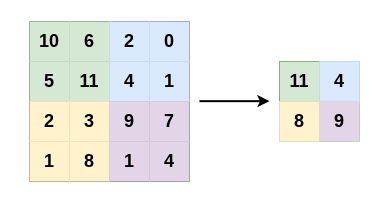
\includegraphics[scale=0.25]{maxpool}
					\caption{Exemplificare a mecanismului de subeșantionare bazat pe funcția maxim. Figura aparține notitelor din cursul CS231n Stanford \cite{standord_cnn}.}
					\label{fig:maxpool}
				\end{figure}
				
				 \noindent Unul dintre beneficiile acestei tehnici, pe lângă reducerea resurselor de memorie și de procesare necesare, este reducerea variației ieșirilor la mici inflexiuni ale datelelor de intrare. Această tehnică încearcă să asigure faptul că modificări care nu ar trebui să influențeze rezultatul nu o să interfereze cu procesul de învățare. \par
				 
				 În crearea unei arhitecturi de rețea neuronală convolutionala, principalii parametrii fixați, pe lângă numărul de nivele, sunt dimensiunea filtrelor pentru fiecare nivel, dimensiunea pasului cu care aceste filtre străbat imaginea și dimensiunea și modul "padding"-ului de la marginea imaginii. "Padding"-ul reprezintă adăugarea unui număr de rânduri sau coloane de diferite valori (de ex 0, sau copii ale anumitor rânduri sau coloane) la marginea imaginii pentru a ne asigura că rezoluția imaginii este divizibilă cu lungimea și lățimea filtrului aplicat..
				
			\section{Rețele neuronale recurente} \label{RNN}
				
				Rețelele neuronale recurente, că și cele convoluționale, sunt specializate pe procearea informației bidimensionale, cu toate acestea diferența apare în faptul că pentru rețele recurente a două dimensiune nu mai este spațială ci temporală. Aceste rețele neuronale primesc datele de intrare într-o manieră secvențială și reușesc să depisteze relațiile temporale dintre două sau mai multe segmente de date aflate la momente de timp diferite. \par
				
				Arhitectura acestei tipologii de rețele neuronale se bazează pe determinarea stării curente a sistemului și transmiterii acesteia celulei aflate la momentul de timp următor. Secretul din spatele rețelelor recurente stă în folosirea aceluiași set de parametrii pentru celulele de la fiecare moment. Astfel având date de intrare organizate secvențial în funcție de timp, $x^{(t)}$, celula unei rețele neuronale recurente folosește o așa zisă "celulă de memorie" pentru a salva starea din momentul t, $h^{(t)}$, și a o transimte ca o a două intrare momentului $t+1$. Folosirea unor parametrii comuni atât pentru procesarea intrărilor $x^{(t)}$ și $h^{(t-1)}$ la momentul $t$ cât și a intrarlor $x^{(t+1)}$ și $h^{(t)}$ la $t+1$ permite rețelei neruonale să determine relațiile temporale între aceste două momente diferite și astfel să ia decizii în prezent bazate și pe informațiile din trecut, Fig. \ref{fig:unfolding}. 
				
				\begin{figure}[h]
					\centering
					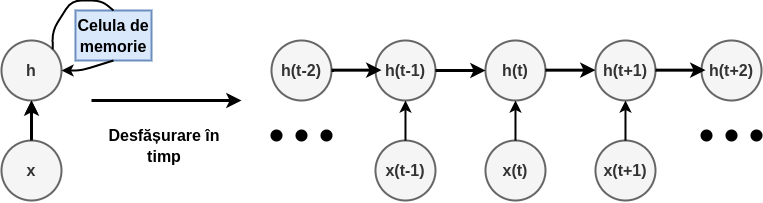
\includegraphics[scale=0.45]{unfolding}
					\caption{Derularea celulei recurente în timp. Figura aparține Goodfellow et al., 2016 \cite{dpb}.}
					\label{fig:unfolding}
				\end{figure}
				
				Celula de memorie este o denumire fictivă, ea referindu-se doar la mecanismul de prezervare a stării curente și transmiterii ei la celula recurentă dintr-un moment viitor. Acest lucru se realizează prin folosirea mai multor seturi de parametrii. Într-o rețea neuronală normală fiecare celulă, neuron, este alcătuită dintr-un singur set de parametrii, ponderi, care se înmulțesc matricial cu datele de intrare rezultând astfel gradul de activare al acelui neuron. Formula care stă la baza computatiilor din interiorul fiecărui neuron pentru o rețea neuronală simplă  este $Y = W^T * X + b$, unde $Y$ este "activarea" neuronului iar $W$ și $b$  reprezintă parametrii antrenați. Dacă un nivel dintr-o rețea neuronală artificială tradițională conține mai mulți neuroni, un nivel al unei rețele recurente este alcătuită dintr-o singură celulă distribuită pe mai multe puncte de timp. Spre deosibire de neuronul unei rețele generice, celulă RNN trebuie să realizeze mai multe sarcini. Pe lângă extragerea informațiilor din datele de intrade curente, de la momentul $t$, celula recurentă trebuie să proceseze și starea de la momentul $t-1$ inanite de a determina ieșirea $y^{(t)}$ și starea curentă $h^{(t)}$. Din acest motiv pentru fiecare din aceste sarcini difeite se alocă un set de ponderii separat, de exemplu $U, W, V$ din Fig. \ref{fig:rnn_layer}.
				
				\begin{figure}[h]
					\centering
					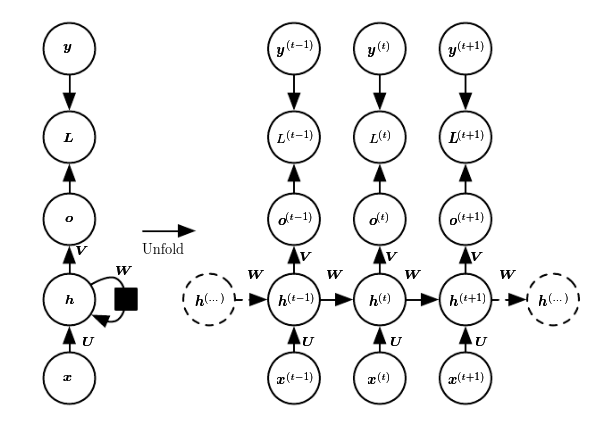
\includegraphics[scale=0.6]{rnn_layer}
					\caption{Desfășurarea procesului de antrenare pe intervalul de timp al datelor de intrare. La fiecare moement $t$ se calculează o eroare $L^{(t)}$ că va genera modificarea tuturor ponderilor din $t$ și momentele predecesoare care au contribuit la această. Figura aparține Goodfellow et al., 2016 \cite{dpb}.}
					\label{fig:rnn_layer}
				\end{figure} 
					Deoarece o celulă recurentă folosește un număr mai mare de parametrii, computațiile din interiorul acesteia devin mult mai complicate. Pentru o rețea neruonala recurentă generică o celulă poate fi descrisă prin următoarele ecuații:
				
				\begin{align}
					a^{(t)} &= b + Wh^{(t-1)} + Ux^{(t)} \\ \label{rnn_states}
					h^{(t)} &= \tanh{(a^{(t)})}\\
					o^{(t)} &= c + Vh^{(t)}	
				\end{align}
				unde $a^{(t)}$ și $h^{(t)}$ reprezintă starea internă a celulei înainte și după aplicarea unei funcții de activare, $o^{(t)}$ reprezintă valoarea la ieșirea celulei, $U$ reprezintă ponderile datelor de intrare, $W$ reprezintă ponderile aferente stării precedente a rețelei și $V$ ponderile de la ieșirea celulei. \par
				
				Deoarece arhitectura unei celule recurente folosete seturi de parametrii diferite pentru cele două intrări, stare precedentă și datele de intrare curente, aceasta poate controla atât impactul informațiilor acumulate din trecut cât și importanța datelor noi observate în prezent. Acești parametrii, împreună cu cei aferenți controlului ieșirilor $V$,  sunt modificați în timpul antrenării din două perspective: reducerea erorii ieșirii celulei de la timpul $t$, $L^{(t)}$,  și reducerea erorii adăugate de folosirea stării curente , $h^{(t)}$, în calculele iesiriilor celuleor de la momentele de timp viitoare, $L^{(t+1)}$, $L^{(t+2)}$, etc. \par
				
				Una din problemele depistate în cazul rețelelor recurente este echilibrarea influenței introduse de stările de la momente de timp îndepărtate comparate cu cele de la momente de timp apropiate. Fiecare celulă recurentă stabilește impactul stariilor precedente printr-o inmulitire matricială cu un anumit set de parametrii, \ref{rnn_states}. Astfel, ponderea informațiilor unei stări dintr-un trecut îndepărtat poate scădea sau crește exponențial. Dacă neglijăm funcția de activare și "bias"-ul, pentru ușurință notației, sistemul de tranziție a informațiilor recurente, stărilor, în timp devine:
				\begin{align*}
				h^{(t)} &=  W^Th^{(t-1)} + U^Tx^{(t)}\\				
				h^{(t)} &=  W^T(W^Th^{(t-2)} + U^Tx^{(t-1)}) + U^Tx^{(t)}\\	
				h^{(t)} &= (W^2)^Th^{(t-2)} + W^TU^Tx^{(t-1)} + U^Tx^{(t)}\\	
				h^{(t)} &= (W^t)^Th^{(0)} + (W^{t-1})^TU^Tx^{(1)}+ ...+ W^TU^Tx^{(t-1)} + U^Tx^{(t)}
				\end{align*}
				Se poate astfel observa cum informațiile obținute la stările anterioare sunt puternic influențate de distanță acestora față de momentul prezent. Deoarece de obicei valorile ponderilor din $W$ sunt initializate cu valori mai mici decât 1, rețelele neuronale recurente tind să uite informațiile din stările incipiente dând o importanță mult mai mare celor din momentele de timp mai apropiate. În multe cazuri acest lucru nu este rezultatul dorit. Un exemplu ar fi crearea unui traducător dintr-o limba A într-o limba B. Sensul unui cuvânt aflat la capătul unei propoziții poate depinde de unul din cuvintele de la începutul propoziției. Dacă traducătorul uită de existența acelui cuvânt traducerea va fi în final una eronată.\par
				
				Pentru rezolvarea acestei probleme s-au propus noi arhitecturi ale celulelor care alcătuiesc rețelele neuronale recurente. Una din aceste arhitecturi, și cea folosită de mine în acest proiect, este "Long Short-Term memory cell", sau LSTM. Diferența dintr-o celulă LSTM și una recurentă normală este folosirea unor așa numite porți care reușesc să îmbunătățească capacitatea celulei de a controla informațiile păstrate sau uitate în procesul de antrenare recurentă.
				
				\begin{figure}[h]
					\centering
					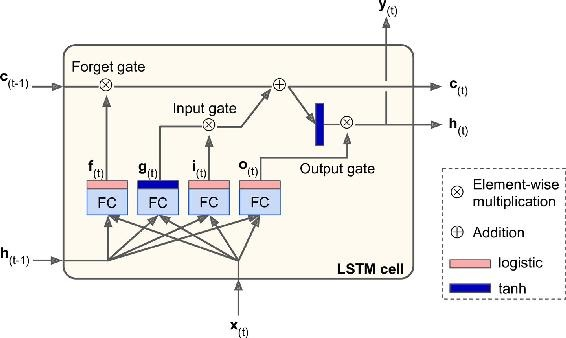
\includegraphics[scale=0.5]{lstm}
					\caption{Structura internă a unei celul recurente LSTM. Se pot observa conexiunile porților care controlează procesele din interiorul celulei: $f_{(t)}$, poarta de uitare, $g_{(t)}$ nivelul de procesare, $i{(t)}$ poarta de intrare și $o_{(t)}$ poarta de ieșire. Figura aparține Gron, 2017 \cite{hands}.}
					\label{fig:lstm}
				\end{figure} 
			
				Celulele LSTM folosesc doi vectori pentru memorarea stării celulei, unul pentru memorarea de lungă durată iar cel de al doilea pentru memorarea pe o durata scurtă. În Fig.\ref{fig:lstm} putem obesrva arhitectura internă a unei astfel de celule și a porților care determina transferul de informație. \par
				Fiecare din aceste porți sunt specializae în timpul antrenării pentru rezolvarea anumitor sarcini specifice:
				\begin{enumerate}
					\item $g(t)$, reprezintă mecanismul principal de procesare de inforamtii din celulă. Valorile obținute la ieșirea acestei părți din celulă reprezintă valorile candidate care ar putea fi introduse în starea celuiei.  Într-o celulă normală, aceste valori ar trece direct în calcularea stării $h(t)$ și ieșirii $y(t)$, fiind aferentul funcției $a(t)$ din \ref{rnn_states}. Într-o celulă LSTM însă, aceste valori sunt filtrate și abia apoi salvate în starea celulei prin folosirea porților.
					\item $f(t)$, este denumită "forget gate", sau poarta de uitare, care controlează care părți din memoria de lungă durată a celulei va fi uitată.
					\item $i(t)$, este denumită "input gate" sau "update gate", și decide ce valori din $g(t)$ ar trebui să fie adăugate la memoria de lungă durată.
					\item $o(t)$, este denumită "output gate", și controlează care părți din memoria de lungă durata ar trebui să fie citite și folosite că ieșiri, atât pentru $h(t)$ cât și pentru $y(t)$. 
				\end{enumerate}
				Se poate observa cum în interiorul celulei LSTM se folosesc două funcții de activare diferite, funcția sigmoid și tanh, prezentate în \ref{ml}. Funcția sigmoid filtrează cantitatea de informație pe care fiecare poartă o cedează mai departe. Fiind urmată de o operație de înmulțire, dacă o valoare din vectorul rezultat este 0 informația aferentă acelei poziții nu este transmisă în continuare. Cu cât acea valoare este mai apropiată de 1 cu atât informația este transmisă mai complet. \par
				Transferul de informație printr-o astfel de celulă se face de la stânga la dreapta, Fig.\ref{fig:lstm}. În primul rând, poarta de uitare, $f(t)$, va filtra memoriile de lungă durata semnificative provenite din $c(t-1)$ luând în considerare memoria de scurtă durata de la momentul anterior, $h(t-1)$, și datele de intrare curente, $x(t)$. Funcția $g(t)$ produce noul set de informații obținute prin combinarea stării trecute cu datele de intrare. Aceste valori sunt apoi înmulțite cu rezultatul porții de "update" care decide care din aceste informații merită stocate în memoria "long-term", fiind adunate la aceasta. După ce varianta reinointa a memoriei de lungă durata este obținută, $c(t)$, este conectată la o ieșire a celulei și la o altă funcție de activare tanh. Poartă de ieșire, $o(t)$, transoformand aceste valori în ieșire celulei, $y(t)$, cât și noua memorie de scurtă-durata, $h(t)$. \par
				Astfel celula LSTM poate să recunoască care din datele de intrare sunt importante și să le stocheze în starea de lungă durata, prin poarta de input, să învețe să le păstreze pentru cât timp sunt relevante , prin poartă de uitare, și să le extragă oricând le consideră necesare, folosind poartă de ieșire. Succesul obținut de celulele LSTM în captarea relațiilor temporale de lungă durata poate fi explicat prin utlizarea acestor succesiuni de porți de control. Totuși, acest succes a fost demonstrat și într-o manieră empirică prin folosirea unor baze de date special concepute pentru această sarcină (Bengio et al., 1994 \cite{rnn3}; Hochreiter and Schmidhuber, 1997 \cite{rnn4}; Hochreiter et al., 2001 \cite{rnn5}) dar și prin aplicarea lor în diferite probleme din lumea inteligenței artificiale. \par
				
				Rețelele neuronale recurente au avut mult succes în recunoașterea emoției în vorbire. Motivul pentru care am ales să folsoesc acest tip de rețele a fost capacitatea acestora de a determina relații temporale între segmentele înregistrărilor audio. Deoarece emoția nu apare doar într-un singur segment, fracțiune de secundă, ci aceasta este prezenta pe întreagă durată a semnalului audio, obținerea  conexiunilor temporale dintre informațiile emoționale prezente în aceste segmente este crucială. 
				
				\section{Mecanismul de atenție} \label{attention}
				 Mecanismului de atenție este bazat  pe principiul de funcționare a percepției umane. Omenii  își focuseaza atenția în mod selectiv, doar pe anumite părți din spațiul vizual sau auditoriu, pentru a extrage informația necesară atunci când este nevoie. Odată extarsa, această informație este combinată cu cea obținută din alte puncte de atenție pentru a crea o reprezentare internă a scenei \cite{zhang, attention1}. \par
				 În SER, acest mecanism are ca scop identificarea segmentelor înregistrării audio cu o mare încărcătură emoțională și îndreptarea atenției modelului pe aceste segmente în timpul antrenării. Din punct de vedere matematic, dorim să obținem un set de parametrii $\alpha_i$, unde $i$ ia valori între 1 și numărul de segmente extrase, $L$, care să funcționeze ca ponderi reprezentative pentru importanța emoțională a fiecărui segment.
				\begin{equation}
					r = \sum_{i=1}^{L} \alpha_i s_i
				\end{equation}
				unde $\alpha_i$ reprezintă ponderea unui segment iar $s_i$ reprezintă datele aferente segmentului $i$. \par
				Mecanismul de atenție poate fi interpretat că o medie ponderată a datelor din fiecare segment. Calcularea ponderilor folosite în această medie se realizează prin adăugarea unui nou nivel de parametrii care vor fi antrenați să depizeteze emoțiile din fiecare segmente în formă următoare.
				\begin{equation} \label{softmax_form}
					\alpha_i = \frac{\exp(w^Th_i)}{\sum_{t=1}^{L} \exp(w^Th_t)}
				\end{equation}
				unde $w$ reprezintă ponderile antrenate.
				Această funcție se numește "softmax" și are ca rezultat un vector egal cu numărul segmentelor extrase. Pentru fiecare segment se obținute un număr între $(0, 1)$, care poate fi interpretat ca probabilitatea ca acel segment să fie bogat în informație emoțională.  Parametrii $w$ sunt antrenați în timpul procesului de învățare împreună cu restul modelului de clasificare.
			
				\section{Cicluri OODA} \label{ooda}
				 Conceptul de ciclu OODA a fost prima dată introdus de strategul militar al Statelor Unite ale Americii, colonelul John Boyd. Boyd susținea că procesul de luare a decizilor decurge într-un ciclu cu 4 stagii principale observare-orientare-decizie-acțiune. Orice entitate care execută acest ciclu mai repede, observând și reacționând la evenimentele care iau loc înaintea oponentului, poate avea un avantaj considerabil și chiar să între în ciclul de decizie al oponentului. Astăzi conceptul de ciclu OODA este folosit în diferite domenii ca afaceri, aplicarea legii, strategii militare și securitate cibernetică. \par
				 
				 În "Machine Learning" aceste cicluri decizionale pot fi adaptapte pentru a eficientiza procesul de antrenare. La fiecare $N$ epocii în timpul procesului de învățare se va extrage câte un set de exemple pentru a reduce timpul în care acest proces are loc. Oponentul în această situație este chiar modelul în sine în versiunea în care folosește întregul set de date de alungul antrenării.  Folosirea acestui mecanism permite grăbirea antrenarii fără a avea efecte negative puternice asupra preciziei modelului. Timpul de învățarea al unui sistem SER este mare din cauza complexității ridicate a problemei, iar prin introducerea acestui mecanism acest interval de timp poate fi aproape înjumătățit. \par
				 
				 În soluția propusă numărul de exemple extrase la fiecare $N$ epoci este stabilit prin formulă următoare:
				 \begin{equation}
				 	D_i = D_{i-1} - \frac{p * D}{\frac{E}{N}}
				 \end{equation}
				  unde $D$ este numărul total de exemple folosite la antrenare, $D_i$ reprezintă numărul de exemple folosite în epoca $i$, $p$ este procentajul de exemple extrase, $E$ este numărul total de epocii iar $N$ este numărul de epocii dintr-un ciclu. \par
				 În această lucrare de diplomă s-au utilizat două moduri de determinare a setului de exemple care urmează să fie extrase, în mod aleatoriu și în funcție de eroarea fiecărui exemplu. Rezultatele pentru ambele cazuri sunt prezentate în capitolul \ref{rezultate}. Această funcționalitate este opțională fiind folosită doar pentru a reduce timpul de antrenare.
		\chapter{Descrierea implementării}
				După cum am menționat și în capitolele anterioare, proiectul meu este alcătuit din două părți principale: modelul "Machine Learning" pentru recunoașterea emoțiilor în semnale audio și interfața grafică pentru utilizator. Prima parte reprezintă soluția propusă pentru consturirea unui model SER iar cea de a două face că această soluție să poată fi antrenată, testată și utilizată într-un mod accesibil, oferind o gama de funcționalități.\par 
				Diagramă din Fig. \ref{fig:uml}, ilustrează distribuția claselor folosite și relațiile dintre acestea. Se poate observa cum există un număr mare de module de procesare de date, aferente diferitelor moduri de extragere a caractersiticitlor semnalului audio dar și a diferitelor funcționalități, ca antrenare și testare, inferență și inferență în timp real (online). Clasa care susține interfață grafică (UI\_MainWindow) apelează aceste moduri de utilizare în funcție de acțiunile utilizatorului. \par
				
				Lucrarea de diplomă a fost implementată în limbajul de programare Python, flolsind cadrul de programare specializat pentru dezvoltarea aplicațiilor Machine Learning, Tensorflow \cite{tensorflow}. Mai exact pentru a eficentiza înmulțirile matriciale care stau la baza oricărei operații din spatele modelelor ML, am folosit o versiune specială numită \textit{tensorflow-gpu}, care realizează oricare astfel de operație matematică folosind placa video. Aceste tipuri de procesare sunt specializate să lucreze cu date din domeniul video, devenind mult mai eficiente când vine vorba de înmulțiri matriciale de dimensiuni mari. Avantajul obținut prin folsoirea acestei versiuni de Tensorflow este mărirea  vitezei de antrenare a modelelor. Pentru extragerea semnalului din fiserele audio, realizarea interfeței grafice și a funcționalității de înregistrarea online am folosit diferite librării specifice prezentate în următoarele subcapitole. \par
				\begin{figure}[p]
					\hspace*{-1,5cm}
					\centering
					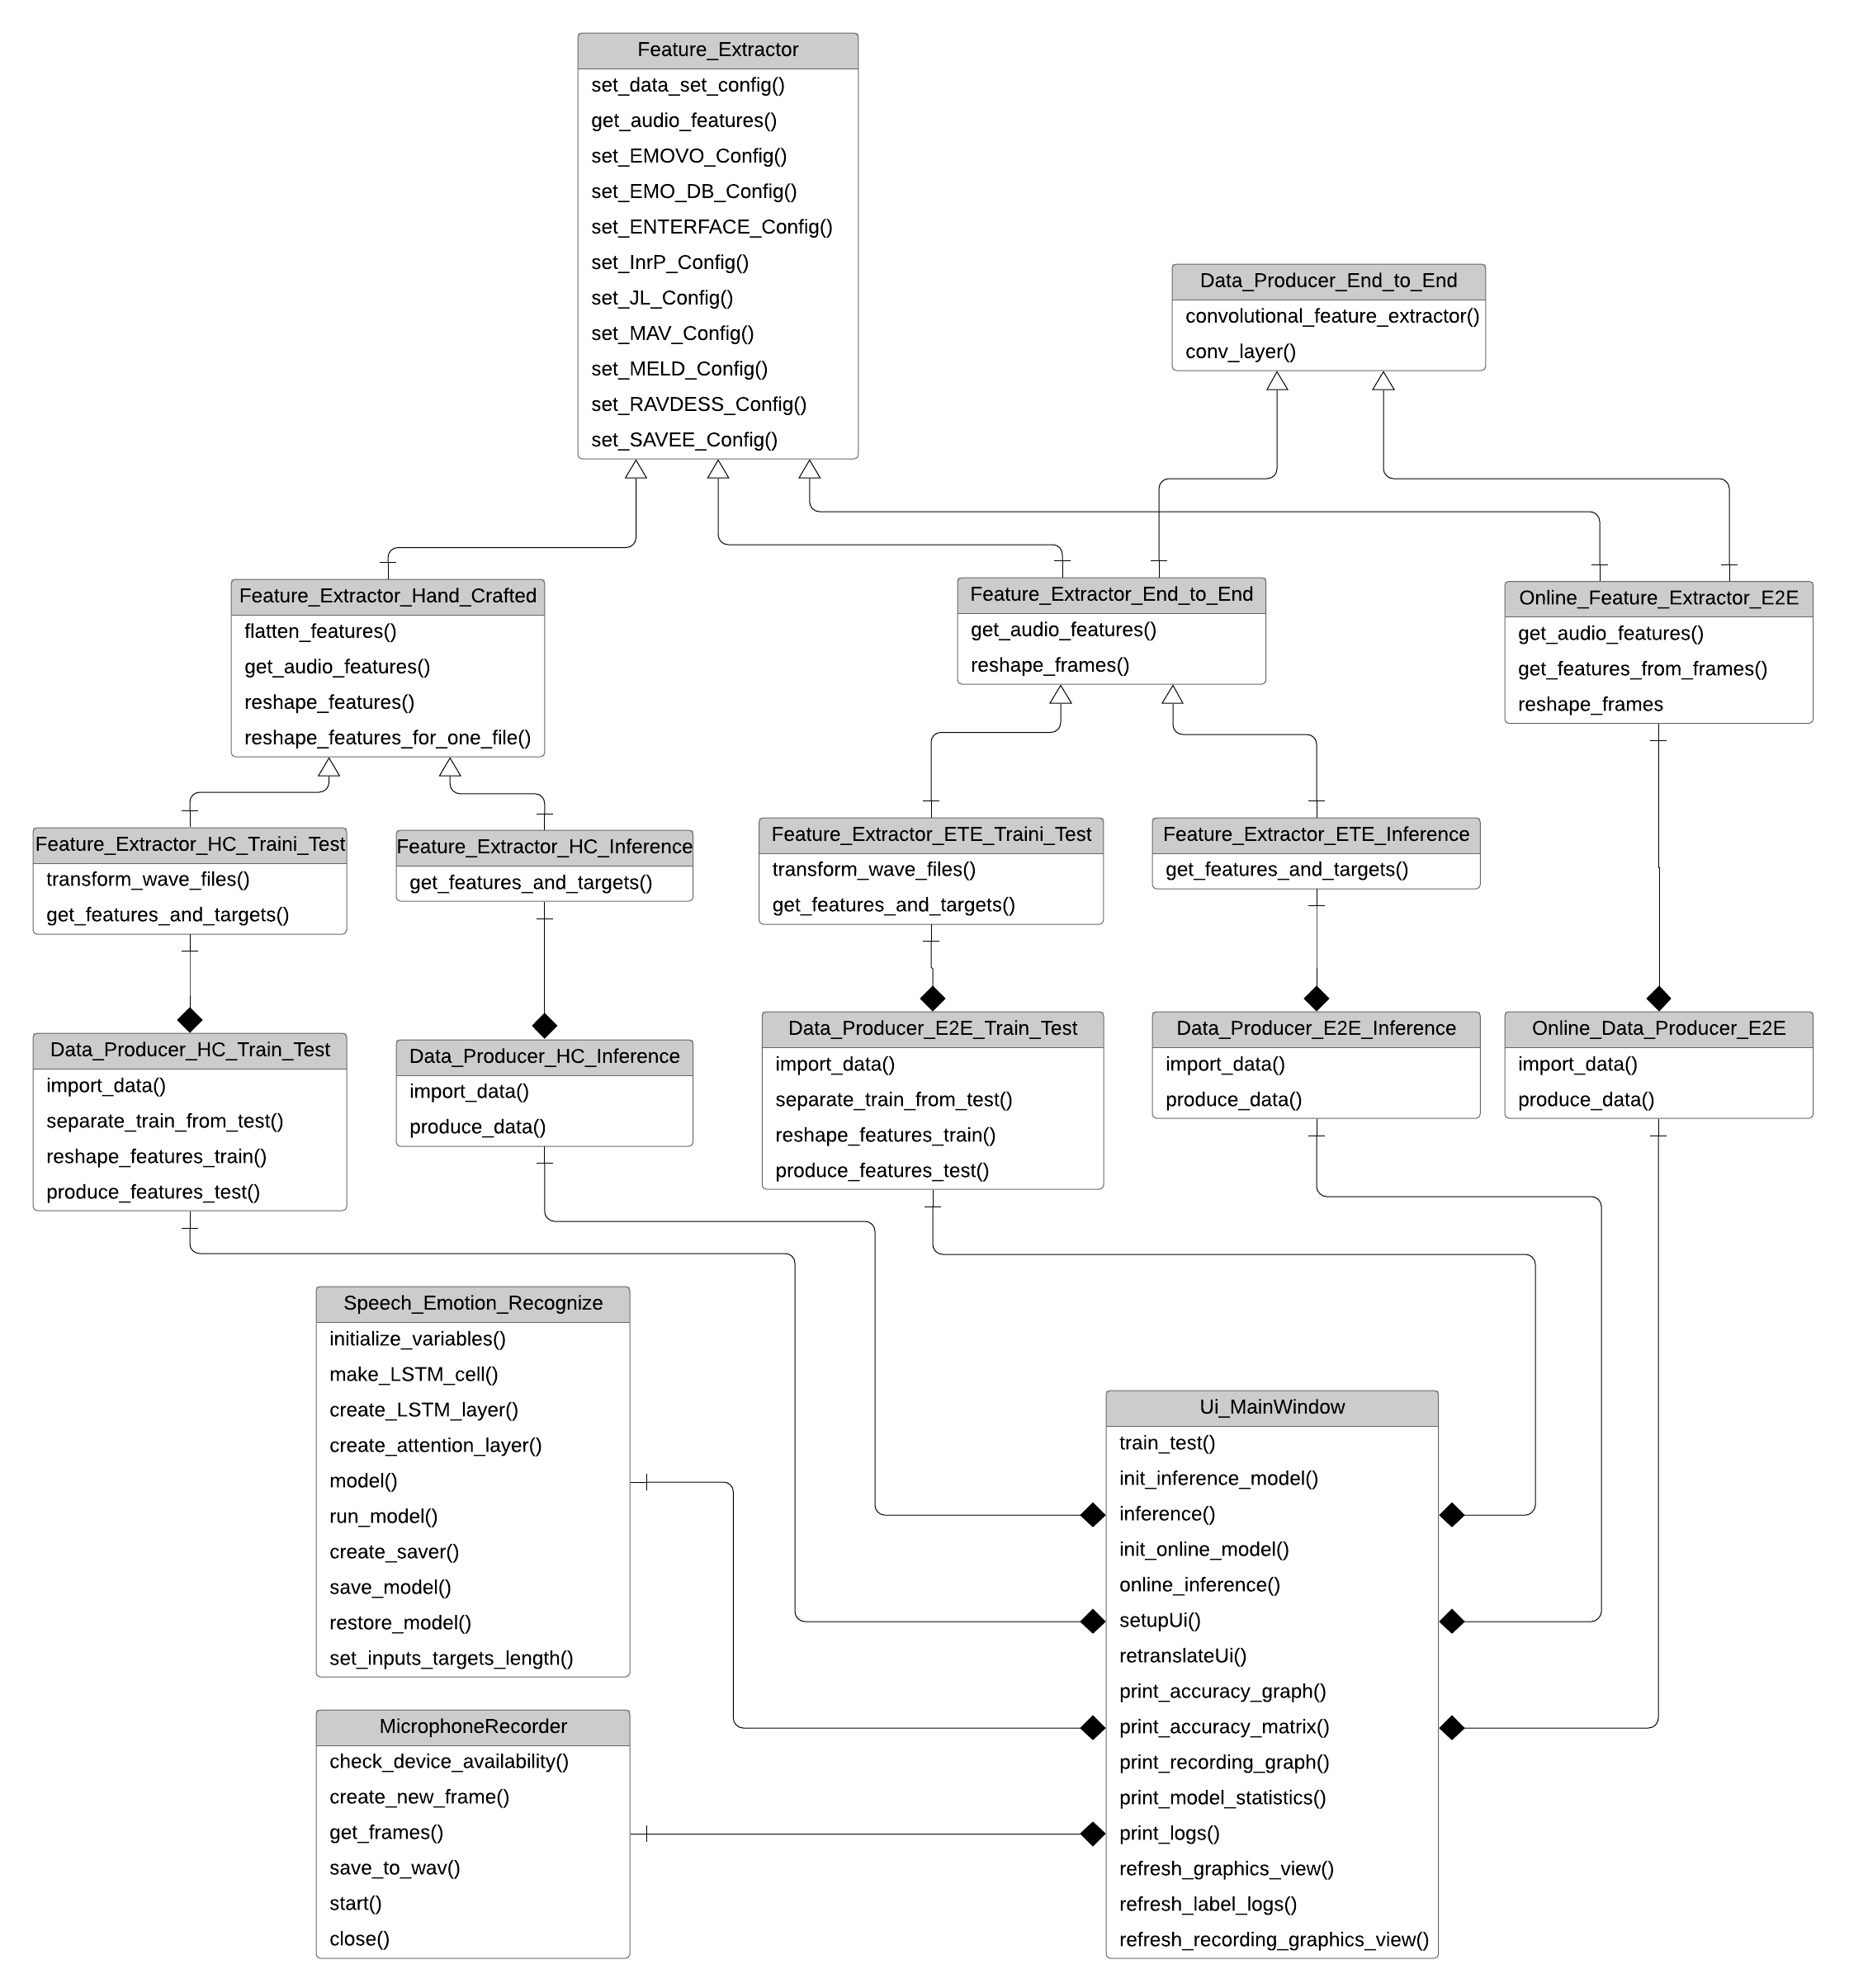
\includegraphics[scale=0.56]{uml}
					\caption{Diagrama UML ilustrativă a distribuției claselor proiectului. Utilizatorul are acces la întregul set de funcționalități al aplicației prin interfață grafică implementată în clasa \textit{UI\_MainWindow}.}
					\label{fig:uml}
				\end{figure} 
			
				\section{Modului de implementare a sistemului de recunoaștere a emoțiilor}
				
				După cum am menționat și în capitolul \ref{introdP}, un model "Machine Learning" de clasificare tipic trebuie să realizeze trei sarcini: preprocesarea datelor, extragerea caracteristicilor de intrare și clasificarea propriu-zisă. Arhitectura propusă de mine pentru realizarea unei soluții pentru problema recunoașterii emoției este ilustrată în Fig. \ref{fig:model}. În capitolul precedent am prezentat o descriere teoretică a algoritmilor folosiți pentru construirea unui astfel de model, urmând că în acest capitol să prezint modul în care aceste concepte teoretice au fost implementate.
				
					\subsection {Bazele de date folosite} \label{datasets}
					În conextul domeniului SER una din principalele probleme este numărul redus de exemple din majoritatea bazelor de date existente. Cu toate că în ultimii ani au apărut baze de date noi, care folosesc un număr mai mare de exemple, acestea nu sunt publice și necesită sume destul de mari de bani pentru accesul la date. Din aceste motive am decis să folosesc mai multe baze de date publice în limbi și configurații de înregistrare diferite. Pe lângă aceste baze de date profesioniste, am decis să adaug și un set de înregistrări proprii pentru a familiariza modelul cu configurațiile microfonului meu și pentru a contribui la majorarea numărului de exemple pentru antrenare.\par
					
					\newpage
					Bazele de date pe care le-am folosit sunt următoarele: EMO-DB, RAVDESS, SAVEE, EMOVO, MAV, ENTERFACE, JL și InrP.
					
					\begin{itemize}
						\item EMO-DB \cite{emodb} este o bază de date în limba germană, conținând aproximativ 500 de înregistrări jucate de 10 actori în contextul a 7 emoții: fericire, enervare, anxietate, frică, plictisire, dezgust și neutru. 
						
						\item RAVDESS \cite{ravdess} conține 1440 de fișiere audio care reprezintă înregistrări jucate de 24 de actori profesioniști aferente a 7 emoții: neutru, fericire, tristețe, enervare, frică, surpindere și dezgust. Limba în care au fost înregistrate aceste emoții jucate a fost engleză, cu un accent nord-american.
						
						%\item SAVEE	
						
						\item EMOVO \cite{emovo} este o baza de date care conține 588 de înregistrări audio a 7 emoții dezgust, frică, enervare, fericire, surpiza, tristețe și neutru. Înregistrările au fost obținute prin angajarea a 6 actori.
						
						\item MAV \cite{mav} sau "Montreal Affective Voices" este alcătuită din 90 de înregistrări nonverbale corespunzând unui set de 8 emoții: enervare, dezgust, frică, durere, tristețe, surprindere, fericire, plăcere și neutru, înregistrate de 10 actori.
						
						\item ENTERFACE \cite{enterface} conține 1320 de înregistrări audio, care surpind 6 emoții: enervare, dezgust, frică, fericire, tristețe și surpindere în 14 limbi diferite.
						
						\item JL \cite{JL} este alcătuită din 2400 înregistrări din 240 de propoziții jucate de 4 actori în contextul a 5 emoții: enervare, tristețe, neutru, fericire, entuziasm.
						
						\item InrP reprezitna setul de exemple personale alcătuit din 320 de înregistrări care cuprind cele 4 emoții clasificate: enervare, tristețe, fericire și neutru.							
					\end{itemize}
				
				\subsection{Preprocesarea datelor}
					Tipul datelor de intrare folosite de modelul propus de mine sunt fișierele audio, mai exact fișierele cu extensia .wav care este cea mai folosită extensie pentru stocarea înregistrărilor audio în bazele de date SER existente. Încărcarea valorilor amplitudinilor semnalului audio într-o matrice de stocare se realizează folosind o librărie specifică pentru porcesarea semnalului audio în Python, numită \textit{librosa} \cite{librosa}. Această librărie oferă o gama largă de funcții pentru procesarea semnalelor audio,  urmând să fie prezentate în subcapitolul explicativ pentru extragerea caracteristicilor de intrare \ref{fex}.
					
					Pentru alcătuirea setului de date am folosit înregistrări din diferitele baze de date prezentate mai sus. Înregistrările fiecărei baze de date au fost realizate folosind diferite frecvențe, variind între 16KHz și 48KHz. Pentru a reduce memoria folosită cât și a  timpului necesar pentru antrenare (de la 12h la aproximativ 4h) am decis să re-esantionez fișierele audio cu o frecvență de 16KHz folosind librăria librosa. Teorema lui Nyquist ne spune că folosind o rată de eșantionare de 16KHz putem surpinde fără pierderi orice semnal cu frecvente mai mici sau egale cu 8KHz. Aceste frecvențe sunt mai mult decât necesare pentru captarea vocii umane, care în contexte normale nu depășește mai mult de 4KHz. Din punct de vedere empiric nu am gaist nici un dezavantaj în a folosit mecanismul de re-eșantionare, sistemul SER obțînând aceași acuratețe în același număr de epoci cu sau fără această tehnică. \par
					
					Înainte ca semnalul audio să poată fi folosit pentru extragerea informațiilor emoționale, acesta trece printr-un proces de partitionare în segmente de lungime fixă. Acest lucru ne permite să aplicăm transformatele Fourier, sau alte funcții asemănătoare, pe porțiuni mai mici din semnalulu inițial, obținând o descriere mai detaliată a acestia. Pentru a reduce datele pierdute între segmente, de obicei se alege un pas de lungime mai mică decât dimensiunea segmentelor. Astfel o parte din informația segmentului actual va fi prezentă și în cel viitor. \par 
					Următoarea etapă a procesului de preprocesare este aplicarea unor funcții fereastara pe fiecare "frame". Acest lucru este realizat pentru a reduce pierderea de informații la aplicarea transformărilor Fourier din cauza discontinuității de la marginea segmentelor. Funcțiile fereastră sunt funcții care converg la zero în afară unui anumit interval. Înmulțind un segment cu o astfel de funcție are ca rezultat dispariția discontinuitatiilor de la marginea segmentului, similar cu privitul printr-o fereastră normală. Funcția fereastră folosită se numește "Hann-window", numită după Julius von Hann, și are formula următoare. \par
					\begin{equation}
					w[n]=\sin^2(\frac{\pi n}{N})
					\end{equation}.
					
				\subsection{Extragerea caracteristicilor de intrare} \label{fex}
				Semnalul audio nemodificat nu este cea mai eficientă modalitate de reprezentare a informației emoționale dintr-un discurs. Din acest motiv există modalități, funcții matematice, care să pună în lumină caracteristicile semnalului audio pentru a putea fi interpretat de sistemele SER în detectarea emoțiilor. Aceste formule aplicate direct pe semnalul audio au fost prezentate în subcapitolul \ref{hand-crafted} pentru caracteristicile de intrare "hand-crafted" și \ref{end-to-end} pentru extragerea antrenabilă a caracteristicilor. \par
				
				În primul caz, extragerea caracteristilor de intrare, ca coeficienții \textit{cepstrali Mel (MFCC)} sau \textit{delas} și \textit{delta-deltas} s-a relizeazat prin folosirea funcțiilor aferente prezente în librăria \textit{librosa}. Pentru ca extragerea acestor date să fie corectă și pentru ca rezultatele obținute să aibe dimensionalitatea dorită a fost nevoie să caluclez lungimea potrivită a segmentelor, mărimea pasului de la un segment la altul, mărimea funcției fereastră etc. \par
				
				\begin{lstlisting}[language=Python, caption={Extragerea caracteristicilor hand-crafted, 3.3, folosind libraria librosa.}, xleftmargin=0cm]
 def _get_audio_features(self, wav_file):
		signal, rate = librosa.load(wav_file,  self.hz)
		mfcc = librosa.feature.mfcc(y=signal, sr=rate, hop_length=260, 
									n_mfcc=20)
		delta = librosa.feature.delta(mfcc)
		delta_deltas = librosa.feature.delta(delta)
		rms = librosa.feature.rms(y=signal, frame_length=640, 
								hop_length=260)
		zcr = librosa.feature.zero_crossing_rate(y=signal, 
								frame_length=640, hop_length=260)
		chroma = librosa.feature.chroma_stft(y=signal, sr=rate, n_fft=820, 
								win_length=640,	hop_length=260)
		rolloff = librosa.feature.spectral_rolloff(y=signal, sr=rate, 
								n_fft=820, win_length=640, hop_length=260)
		features = [mfcc, delta, delta_deltas, rms, zcr, chroma, rolloff]
		return features	\end{lstlisting}
				
				În cel de al doilea caz am folosit librăria librosa doar pentru a aduce semnalul audio la o formă care eficientizează procesul de antrenare al rețelelor neuronale convoluționale. Astfel am extras spectograma Mel, \ref{mel}, folosind funcția corespunzătoare din librăria \textit{librosa}. Rezultatul obținut este o imagine de dimensiuni 128x128 pentru fiecare din segmentele semnalului audio. Această imagine este apoi normalizată și transmisă rețelei convoluționale care se ocupă cu extragerea automată a informației emoționale. Deoarece rețeaua convoluțională este la rândul ei antrenată în timpul procesului de învățare, caracteristicile extrase de aceasta vor fi mai specifice sarcinii de recunoaștere a emoției decât cele folosite în metodă "hand-crafted". \par
				
				\begin{lstlisting}[language=Python, caption={Extragerea spectogramei Mel, 3.4.1, folosind libraria librosa.}, xleftmargin=0cm]
  def _get_audio_features(self, wav_file):
		signal, _ = librosa.load(wav_file, self.hz)
		librosa.core.time_to_frames
		stft = librosa.feature.melspectrogram(signal, n_fft=512, 
							   win_length=128, hop_length=32, center=False)
		return stft	\end{lstlisting} \par
				Arhitectura rețelei convoluționale folosite este prezentată în \ref{end-to-end}, iar secvența de cod care realizează această funcționalitate este ilustrată în Alg. \ref{cnn_code}. \par 
				Funcția \_convolutional\_feature\_extractor este responsabilă pentru crearea modelului rețelei convoluționale. Parametrul de intrare \textit{stft} reprezintă vectorul de spectograme Mel aferente segmentelor unei anumite înregistrări și este transmis primului nivel al rețelei convoluționale. \par
				Fiecare nivel al rețelei convoluționale este constiuit folosind metoda \textit{conv\_layer}. În această metodă se crează parametrii antrenabili din fiecare nivel, Alg.\ref{cnn_code} linia 5, în funcție de dimensiunea filtrelor și a datelor de intrare. Parametrii obținuți sunt transmiși funcției \textit{tf.nn.conv2d} a librăriei Tensorflow care va crea nivelul convolutional specializat pe date în două dimensiuni. \par
				Pentru primul nivel dimensiunea filtrelor a fost aleasă de \textit{8x8x1} pixeli iar numărul acestor filtrii este de 32, \textit{channels\_out}. Între nivele rețelei am folosit funcția de activare $tanh$, urmată de funcția de subesantionare maxim din librăria Tensorflow, \textit{tf.nn.max\_pool}. Motivația folosirii acestor funcții fiind descrise în secțiunile \ref{ml} respectiv \ref{cnns}.
				
				Tehnică numită "batch normalization", \ref{batch-norn}, este implementată prin normalizarea  valorilor rezultate în urmă funcției  "max\_pooling" după fiecare nivel al acestei rețele. \par 
				
				Cel de-al doilea nivel este construit în aceeași modalitate că și primul doar că conține 16 filtre de dimensiunea \textit{4x4x32}. La final rezultatul care ajunge să aibă dimensiunea \textit{(4 * nr\_segmente)x16x16} este aplatizat și adus la forma \textit{(4*nr\_segmente)x256} pentru a deservi ca intrare pentru rețeaua neuronală recurentă. 
				\begin{lstlisting}[language=Python, caption={Implementarea nivelelor convoluționale care realizează extragerea caracteristicilor în manieră end-to-end folosind procedurile librăriei Tensorflow.}, xleftmargin=-1cm, label=cnn_code]
class Data_Producer_End_to_End(object):
	def conv_layer(self, input_data, filter_size, channels_in, channels_out, 
						strides, conv_layer_dropout, name="Conv"):
		W = tf.get_variable("Weights_"+name+"_Layer", dtype=tf.float32, 
				shape=[filter_size, filter_size, channels_in, channels_out])
		return tf.nn.tanh(tf.nn.dropout(tf.nn.conv2d(input=input_data, 
													filter=W, 
													strides=strides, 
													padding='SAME', 
													use_cudnn_on_gpu=True), 
													conv_layer_dropout))
					
	def _convolutional_feature_extractor(self, stft, conv_layer_dropout):
			self.init = tf.glorot_normal_initializer()
			with tf.variable_scope("Convbb", reuse=tf.AUTO_REUSE, 
									initializer=self.init):
				stft = batch_normalization(stft)
				conv1 = self.conv_layer(input_data=tf.expand_dims(stft,axis=3),
										filter_size=8, 
										channels_in=1, 
										channels_out=32, 
										strides=[1, 2, 2, 1], 
										conv_layer_dropout=conv_layer_dropout, 
										name="conv1")			
				conv2 = tf.nn.max_pool(conv1, [1,2,2,1], [1,2,2,1], 
										padding="SAME")
				conv2 = batch_normalization(conv2)
				conv3 = self.conv_layer(input_data=conv2, 
										filter_size=4, 
										channels_in=32,
										channels_out=16, 
										strides=[1, 2, 2, 1], 										conv_layer_dropout=conv_layer_dropout, 
										name="conv2")				
				conv3 = tf.nn.max_pool(conv3, [1,2,2,1], [1,2,2,1], 
										padding="SAME")
				conv3 = batch_normalization(conv3)
				conv_out = tf.reshape(conv3, (-1, 256))
				return conv_out	\end{lstlisting}		
			
			\subsection{Clasificatorul sistemului SER} \label{clasif_prac}
				În Fig.\ref{fig:model} se poate observa cum modulul clasificator este alcătuit din două celule bidirecționale recurente pe două nivele urmat de mecanismul de atenție și de un nivel neuronal "dens". Fiecare din aceste componente aduce un anumit avantaj arhitectural care urmează să fie prezenat în continuare. \par 
				
				Rețelele recurente, \ref{RNN}, spre deosebire de alte tipuri de rețele neuronale reușesc să determine atât informațiile emoționale de la un anumit moment de timp, cât  și relațiile temporale între emoții din diferite momente. Astfel emoțile prezente în începutul înregistrării o să aibe o anumită influență și asupra emoțiilor recunoscute la finalul acesteia. În construirea modulului neuronal recurent am decis să folosesc două celule LSTM bidirecționale, \ref{fig:lstm}, pentru a marii acuratețea sistemului SER. Termenul bidirecțional înseamnă că o celulă va procesa înregistrarea de la început spre final în timp ce cea de a două va procesa aceași informație în sens invers, de la final spre început. În mod normal rețelele recurente se folsoesc de informația actuală și cea din trecut pentru a lua decizia la momentul curent, totuși există aplicații, că și SER, unde decizia la momentul $t$ poate fi influențată și de date prezente la $t+1$. Un exemplu ar fi "speech recognition", unde intonația unei litere poate depinde de litera care o urmază, "co-articulație", sau chiar de cuvintele următoare ( e.g. cuvântul "the" în limba engleză se pronunță diferit dacă e urmat de un cuvânt care începe cu o vocală sau consoană). În recunoașterea de emoții în vorbire emoția fluctuează într-o conversație. Oamenii pot intuii anumite expresii de astfel emoții, de exemplu când cineva spune o glumă și bufnește în ras la final. Algorimtii de detecție a emoțiilor ar trebui să reușească și ei să se folosească de informații viitoare, "intuiri", pentru a determina emoția din prezent. \par Pentru a marii numărul gradelor de libertate ale rețelei recurente, și în final măririi acurateții modelului, am folosit pentru ambele tipuri de traversări ale semnalului audio două nivele neuronale. Secțiunea de cod aferentă acestui modul este prezentată mai jos.\par 

				\begin{lstlisting}[language=Python, caption={Implementarea celulelor LSTM bidirectionale pe doua nivele folosind procedurile specifice ale librariei Tensorflow.}, xleftmargin=0cm]
def make_lstm_cell(self, hidden_size):
	cell = tf.contrib.rnn.LSTMCell(num_units=hidden_size, 
							use_peepholes=True, 		
							initializer=tf.glorot_uniform_initializer())
	if self._is_training and self._keep_prob < 1:
		cell = tf.contrib.rnn.DropoutWrapper(cell, 
										input_keep_prob=self._keep_prob,
										output_keep_prob=self._keep_prob, 
										variational_recurrent=True, 
										dtype=tf.float32, 
										input_size=hidden_size)
	return cell

def create_LSTM_layer(self, inputs, hid_size, name=None):
	with tf.variable_scope(name):
		lstm_cells_fw = [self.make_lstm_cell(hid_size) for _ in range(2)]
		lstm_cells_bw = [self.make_lstm_cell(hid_size) for _ in range(2)]
		multi_cell_fw = tf.contrib.rnn.MultiRNNCell(lstm_cells_fw, 
												state_is_tuple=True)
		multi_cell_bw = tf.contrib.rnn.MultiRNNCell(lstm_cells_bw, 
												state_is_tuple=True)
		initial_zero_state_fw = multi_cell_fw.zero_state(1, tf.float32)
		initial_zero_state_bw = multi_cell_bw.zero_state(1, tf.float32)
		inputs = tf.expand_dims(inputs, axis=0)
		outputs, _ = tf.nn.bidirectional_dynamic_rnn(multi_cell_fw, 
									multi_cell_bw, inputs, 
									initial_state_fw=initial_zero_state_fw, 
									initial_state_bw=initial_zero_state_bw)
		return tf.concat(outputs, 2)[0]				\end{lstlisting}
		Prima funcție, \textit{make\_lstm\_cell} va crea celula recurentă LSTM, primind ca parametrii numărul de "neuroni" interni, care este egal pentru fiecare poartă, \textit{hidden\_size}. Dacă modelul se află în timpul procesului de antrenare se poate folosii tehnica de regularizare numită \textit{dropout}. Această tehnică va dezactiva o anumită parte (1 - \textit{keep\_prob}) din rețeaua recurentă în mod aleator pentru fiecare tranziție prin rețea. Prn acest mecanism se elimina dependențele puternice între neuroni, care poate duce la procesul de "overfitting". Fenomenul de "overfitting" apare atunci când modelul devine mult prea bine specializat pe datele de antrenare și ajunge să nu generalizeze bine pe datele de test, având rezultate slabe în acest caz. \par
		Funcția \textit{create\_LSTM\_layer} este cea care crează întreg modulul recurent prin concatenarea celulelor recurente generate de  \textit{make\_lstm\_cell}. În listele \textit{lstm\_cells\_fw} și \textit{lstm\_cells\_bw} sunt stocate cele două nivele recurente, celule LSTM,  care sunt date apoi ca parametru functiei din librăria Tensorflow \cite{tensorflow}, \textit{tf.nn.bidirectional\_dynamic\_rnn}. Această funcție va crea rețeaua neuronală, oferind celulelor din \textit{lstm\_cells\_fw} datele de intrare în de la început spre sfârșit și celor din \textit{lstm\_cells\_bw} în sens invers. Rezultatele celor două seturi de nivele recurente este salvat în \textit{outputs}. Varianta concatenată este returnată de această funcție, reprezentând ieșirile acestui modul. \par
		
		Rezultatele care reies în urmă procesării recurente a datelor sunt transmise mecanismului de atenție prezentat în \ref{attention}. Cum am spus și mai sus această parte a sistemului SER are rolul de accentua informațiile din segmentele bogate în emoții și de a le neglija pe cele care pot să aducă o notă de ambiguitate în procesul de clasificare. \par
		
		\begin{lstlisting}[language=Python, caption={Metoda care implementeaza mecanismul de atentie, \ref{attention}.}]	
def create_attention_layer(self, frame_predictions, weigths_dim):
	W = tf.get_variable("Attention_Weights", dtype=tf.float32, 
					shape=[weigths_dim, 1])
	b = tf.get_variable("Attention_Bias", dtype=tf.float32, shape=[1])	
	alpha = tf.matmul(frame_predictions, W) + b
	alpha = tf.nn.softmax(alpha, axis=0)
	return tf.expand_dims(tf.reduce_sum(tf.multiply(frame_predictions, 
						alpha[: tf.newaxis]), axis=0), axis=0)		\end{lstlisting}		
		Funcția care implementează tehinca de atenție este destul de scurtă. În prmul rând, se crează ponderile $W$ și "bias"-ul $b$ cu dimenisunea rezultatelor modulului recurent aferente fiecărui segment. Aceste ponderi sunt înmulțite matricial cu datele fiecărui segment urmate de aplicarea funcției \textit{softmax} \ref{softmax_form} pe rezultate. În acest moment fiecărui segment i s-a atribuit un coeficient de "importanță" \textit{alpha}, rămânând doar că acești coeficenti să fie înmulțiți cu valorile rezultate în urmă modulului recurent și să se adune valorile obținute pentru a realiza suma ponderată descrisă și la  \ref{attention}. \par
		
		Odată ce mecanismul de atenție a fost folosit, informațiile din diferitele segmente ale semnalului audio au fost comasate într-un singur set obținându-se astfel rezumatul informației emoționale a întregii înregistrării audio. Acest set este transmis unui nivel neuronal simplu care are rolul de a reduce dimensiunea acestui rezumat emoțional și de a oferi la ieșire probabilitatea ca înregistrarea curentă să aparțină uneia din celor 4 emoții clasificate: enervare, fericire, tristețe și neutru. \par
		
		Funcția care leagă toate aceste componente și crează modelul propus în arhitectura din \ref{fig:model} este următoarea.
		
		\begin{lstlisting}[language=Python, caption={Functia care creaza graficul de executie Tensorflow, conectand toate componentele de procesare ale sistemului SER.}]	
def model(self):
	with tf.variable_scope("Speech_Emotion_Recognizer", reuse=tf.AUTO_REUSE
						,initializer=self.init):
		rnn_layer = self.create_LSTM_layer(self._inputs, 
										self._hidden_size, 
										"Reccurent_Module")		
		attention_layer_output = self.create_attention_layer(rnn_layer, 
												self._hidden_size*2)
		predictions_1 = tf.layers.dense(attention_layer_output, 
										self._emotion_number, 
										name="Output_Layer")
		predictions = tf.reduce_sum(predictions_1, axis=0)		
		targets_raw_ = tf.nn.softmax(predictions, axis=0)		
		targets_ = tf.cast(tf.equal(targets_raw_, 
									tf.reduce_max(targets_raw_)), 
									tf.float32)
		if self._is_inference:
			self.predictions_raw = targets_
			self.predictions = targets_raw_
				return					
		self.label_pred = tf.argmax(targets_raw_)
		self.label_true = tf.argmax(self._targets)		
		self.accuracy = tf.cast(tf.equal(self.label_pred, self.label_true),
								tf.float32)
		if not self._is_training:
			return
		cross_entropy = tf.nn.softmax_cross_entropy_with_logits_v2(
													labels=self._targets, 
													logits=predictions)	
		adam_opt = tf.train.AdamOptimizer(self._learning_rate)
		self.optimizer = adam_opt.minimize(cross_entropy)	\end{lstlisting}
		Funcția \textit{model} folosește caracteristicile extrase de rețeaua convolutionala în cazul end-to-end sau de formulele matematice predefinite în cazul hand-crafted prin parametru \textit{self.\_inputs}. Aceste caracteristici sunt transmise modulului recurent care este apoit conectat la mecanismul de atenție și la nivelul reteli neuronale dense numit "Output\_Layer". Rezultatele acestui nivel au dimensiunea \textit{self.\_emotion\_number}, în cazul nostru 4, pe care se aplică funcția \textit{softmax} pentru a fi reprezntative din punct de vedere probabilistic. Pentru a fi aduse într-un format de genul [0,0,1,0], rezultatele sunt comparate cu probabilitatea maximă, memorând 1 dacă sunt egale și 0 în caz contrar. \par
		
		Dacă modelul este folosit în cazul de inferență după linia 17 se returnează predicția obținută, care este afișată în interfață grafică. \par
		În schimb, dacă se execută procesul de testare este salvată emoția clasificată și cea adevărată pentru crearea statisticilor ilustrate în interfața cu utilizatorul și se determină dacă predicția a avut succes (dacă emoția clasificată este egală cu cea adevărată) la linia 23. \par
		În cazul în care modelul se află în timpul antrenării se calculează eroarea, sau mai exact funcția de "loss", care ne spune exact cât de departe a fost modelul de a prezice corect emoția. Funcția folosită de obicei în cazul clasificării de mai multe clase mutual exclusive se numește "cross entropy", $L = -\sum_{i=1}^{K} y_i \log(P_i)$ unde $K$ este numărul de clase, $y_i$ este valoare adevărată a clasei i (0 sau 1) iar $P_i$ este probabilitatea clasei $i$. Dacă $y_i$ are valoarea 1, iar probabilitatea este apropiată de 1 atunci eroarea, L, are o valoare foarte mică. În schimb dacă probabilitatea este mică prin aplicarea logaritmului negativ se va obține o valoare a erorii mare. \par
		Această valoare a erorii, alături de rată de antrenare, sunt oferite ca parametru de intrare unui optimizator care are rolul de a realiza mecanismul numit "backtracking", prin care se vor actualiza valorile ponderilor din interiorul rețelei neuronală convoluțională, recurentă, mecanismul de atenție și cea densă, pentru a reduce eroarea determinată la pasul curent. Optimizatorul folosit este numit Adam \cite{adam} ("Adaptive momement estimation") deoarece este mult mai rapid decât tipurile de optimizatori tradiționali ca, "gradiend descent". Acest optimizator fiind o extensie a algoritmului "gradient descent"	care folosește diferite rate de învățare pentru parametrii interni și așa numite "momente" care sunt funcții matematice care determină când învățarea poate fi accelerată fără pierderea acurateții. Eficiența acestui algoritm a fost demonstrată in varioase implementări, fiind unul dintre cei mai folosiți optimizatori in domeniul "Machine Learning".
		
	\section{Implementarea și utilizarea interfeței grafice}
		Interfața cu utilizatorul oferă două moduri de utilizare, pentru antrenare și pentru inferență. Primul mod permite utilizatorului să aleagă diferite configurații de parametrii pentru antrenarea modelului și să observe statistici în timp real asupra evoluției acestuia. Cel de al doilea mod este orientat pe partea aplicativă a sistemului SER, permițând utilizatorului să determine emoția predominantă din diferite fiesre audio pre-înregistrate sau chiar să își inregistreze propriul discurs pentru inferență. Cele două moduri de utilizare vor fi descrise în subcapitolele următoare, împreună cu câteva imagini care prezintă interfața grafică. \par 
		Utilizatorul poate alege pe care din cele două moduri dorește să le folosească prin două butoane radio \textit{Train} și \textit{Inference}. Butonul \textit{Start} începe să execute acțiunea aleasă anterior. \par
		
		Pentru realizarea acestei interfețe am folosit librăria PyQt5, care este o varianta a celebrei librării pentru realizarea elementelor grafice din limbajul de programare C++. Tema folosită pentru aplicație a fost realizată în librăria qdarkgraystyle, oferind culoarea și textura entitatiilor grafice din interfață, ca butoane, comboBox-uri etc. 
		
		\subsection{Interfața grafică în modul de antrenare} \label{guiAntrenare}
		
		\begin{figure}[h]					
			\hspace{0.75cm}
			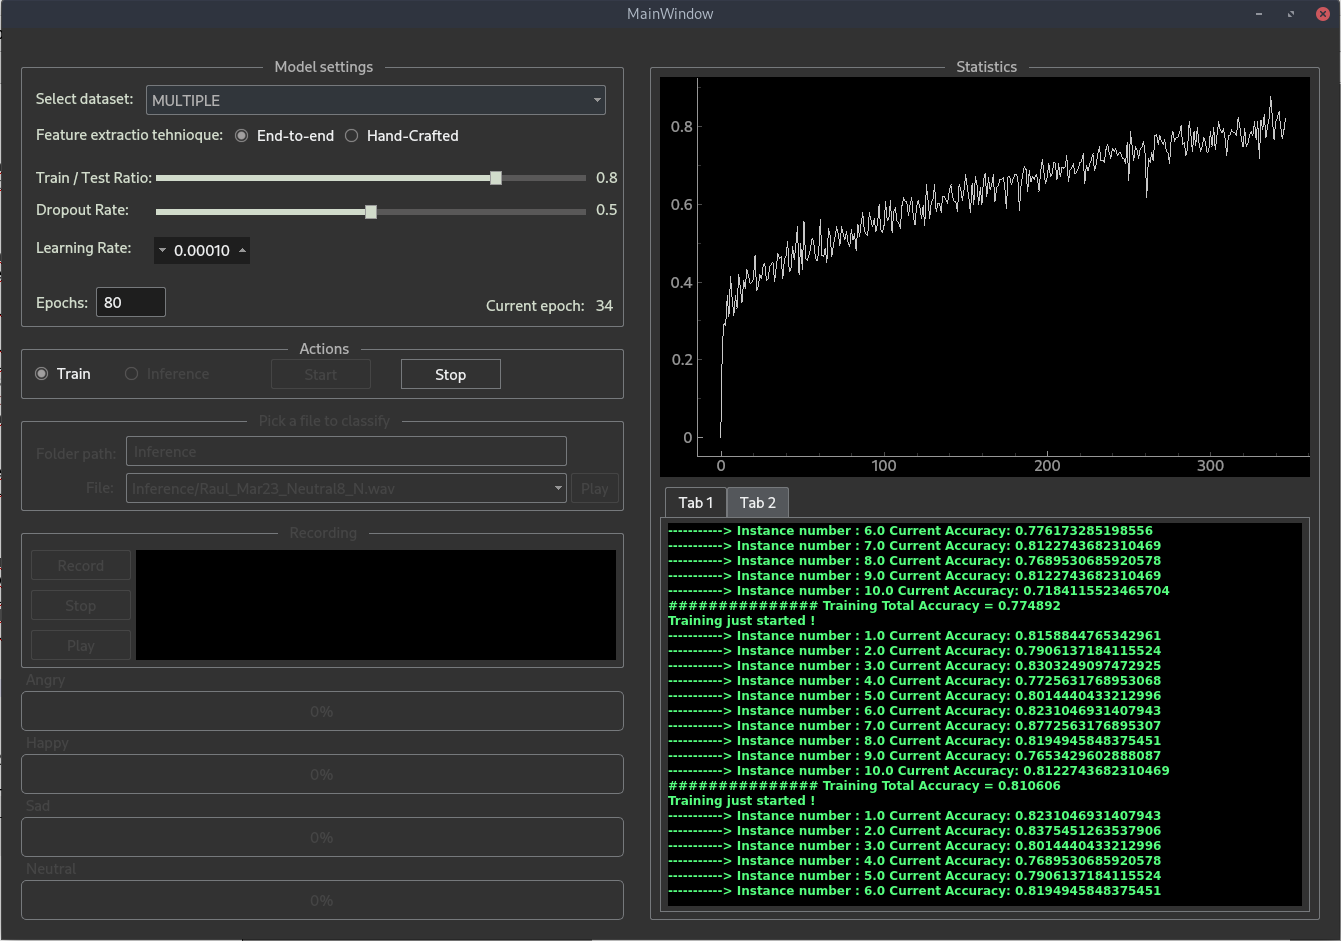
\includegraphics[scale=0.33]{gui_training}
			\caption{Interfață grafică în modul de antrenare}
			\label{fig:gui_train_1}
		\end{figure} 
		
		Interfața grafică în modul de antrenare, ilustrat în Fig. \ref{fig:gui_train_1}, oferă în partea stângă o serie de funcționalități de editare a parametriilor modelului în timp ce în partea dreaptă se poate observa un grafic care prezintă evoluția modelului în timpul antrenarii și statisticile determinate în timpul procesului de învățare. \par
		În secțiunea "Model setttings" din interfața grafică utilizatorul poate să controlzeze contextul în care se execută procesul de antrenare prin intermediul următorului set de parametrii:
		\begin{itemize}
			\setlength{\leftmargin}{-4cm}
			\item \textit{Select dataset}, este un comboBox care listează setul de baze de date care pot fi folosite pentru antrenare. Utilizatorul poate să aleagă una dintre ele sau opțiune Multiple, unde un număr din acestea au fost alese pentru a facilita opțiunea folosirii unui număr mai mare de baze de date într-o antrenare de tip "multi-domain".
			\item \textit{Feature extraction tehnique}, prezintă două butoane tip radio prin care utilizatorul poate decide modul în care sunt extrase caracteristicile de intrare din semnalul audio. 
			\item \textit{Train/Test Ratio} este un slider orizontal care permite utilizatorului să decidă rația din setul de date utilizată pentru antrenare din baza de date aleasă la \textit{Select dataset}. Restul exemplelor vor fi folosite pentru testare. 
			\item \textit{Dropout Rate}, este la fel un slider orizontal prin care utilizatorul decide probabilitatea ca un neuron să fie activ în timpul antrenării. Această tehnică a fost prezentată și în \ref{clasif_prac}. 
			\item \textit{Learning Rate}, este un text editabil prin care utilizatorul poate să decidă rată cu care se vor modifica ponderile în timpul antrenării. 
			\item \textit{OODA loop}, este un checkBox prin care se introduce modul de antrenare "rapid". Sliderul alăturat determină procentul din setul de exemple de intrare care va fi extras folosind algoritmul prezentat la \ref{ooda}. Inițial această funcționalitate este dezactivată dar poate fi activată de utilizator pentru a reduce timpul de antrenare. 
			\item \textit{Epochs}, este un text editabil în care utilizatorul menționează numărul de epoci rulate în timpul antrenării.
			\item \textit{Current epoch}, este un câmp text needitabil care printează epoca în care se află la acel moment procesul de învățare.			
		\end{itemize}
		Aplicația setează o configurație de parametrii recomandată la pornire dar utilizatorul poate să facă diferite încercări modificând câmpurile sugerate mai sus. După ce parametrii au fost setați, prin apăsarea butonului \textit{Start} se începe antrenarea modelului. Deoarece am dorit să prezint starea modelului în timp real pe parcursul învățării, a fost nevoie să creez un nou fir de execuție pentru antrenare după apăsarea butonului \textit{Start}. La anumite momente modelul va genera un set de informații car vor fi transmise firului de execuție principal pentru a le ilustra în zonele grafice aferente. Dacă butonul care setează modul de execuție este în starea \textit{Inference}, \textit{app.radioButton\_2}, apăsarea butonului \textit{Start} va realiza clasificarea unuia din fiserele audio prezentă în directorul \textit{Inference}.
		
		\begin{lstlisting}[language=Python, caption={Metoda interfetei grafice apelata automat in urma apasarii butonului Start.}, label=on_click]	
def on_start_button_clicked(app):
	global thread_train
	if app.radioButton.isChecked():
		app.refresh_label_7()
		app.refresh_graphics_view()
		thread_train = Train_App(app)
		thread_train.print_accuracy_signal.connect(app.print_accuracy_graph)
		thread_train.print_stats.connect(app.print_stats_model)
		thread_train.print_matrix.connect(app.print_accuracy_matrix)
		thread_train.print_epoch.connect(app.print_label_19)
		thread_train.start()
	elif app.radioButton_2.isChecked():
		global ses, ser_inference_model, files
		vals = inference(ses, ser_inference_model, files ,
							app.comboBox_2.currentText()) * 100
	pass \end{lstlisting}
		\textit{Train\_App} reprezintă noul fir de execuție cu ajutorul căruia se va antrena modelul. În secvența de cod de mai jos se poate observa cum clasa \textit{Train\_App} moștenește \textit{QtCore.QThread}. Odată instanțată această clasă apelează funcția \textit{run}, care conține apelul către funcția \textit{train}, care pornește procesul de învățare a modelului SER.
		\begin{lstlisting}[language=Python, caption={Clasa aferenta firului de executie pentru procesul de antrenare.}]	
class Train_App(QtCore.QThread):
	print_accuracy_signal = QtCore.pyqtSignal(float)
	print_stats = QtCore.pyqtSignal(str)
	print_matrix = QtCore.pyqtSignal(object)
	print_epoch = QtCore.pyqtSignal(str)
	stopFlag = False
	def __init__(self, app_rnning, parent=None):
		QtCore.QThread.__init__(self, parent)
		self.app_rnning = app_rnning
		
	def run(self):
		train(self, int(self.app_rnning.lineEdit.text()),
				float(self.app_rnning.horizontalSlider_2.value()) / 10,  
				float(self.app_rnning.horizontalSlider.value()) / 10, 
				float(self.app_rnning.doubleSpinBox.value()) ,
				map_config[self.app_rnning.comboBox.currentText()], 
				self.app_rnning.radioButton_3.isChecked()) \end{lstlisting}
		Funcția train primește parametrii care crează contextul de execuție al modelului, prezentați anterior, și începe procesul de antrenare. În interiorul acestei funcții se resetează graficul de execuție \textit{Tensorflow} pentru procesul actual, se crează nouă sesiune \textit{Tensorflow}  pe care vom rula modelul, se crează și apelează clasa care extrage caracteristicile de intrare din înregistrările audio și începe procesul de învățare. La finalul antrenării este apelat modelul testor iar modelul antrenat este salvat pentru a putea fi folosit în modul de utilizare pentru inferență. \par
		
		Statisticile sunt realizate în timp real prin intermediul informațiilor transmise din cadrul procesului de învățare. Librăria PyQt5 folosește conceptul de semnale pentru actualizarea informațiilor din interfețele grafice. Astfel un semnal este emis din firul de execuție pentru antrenare printr-o funcție care este "conectată" la cea care modifică interfața grafică. Această funcție "conectoare" face parte din clasa firului de execuție și modul de utilizare este ilustrat în 
		secvența de cod \ref{on_click}. \par
		Prima statistică ilustrată în interiorul apilcatiei este graficul care prezintă evoluția acurateții modelului în timpul antrenării. Acest grafic poate fi folosit pentru a determina anumite probleme care pot să apară în timpul antrenării sau pentru a determina cel mai favorabil număr de epoci. \par
		Cea de a două statistică este una multiplă, fiind alcătuită din două pagini. Prima pagină are rolul de a înștința utilizatorul legat de procesele care i-au parte în interiorul modelului, de exemplu extragerea datelor dintr-un anumit set sau acuratețea atinsă pe datele de antrenare într-o anumită epoca, și este ilustrată în Fig \ref{Fig:gui_train_logs}. Cea de a două pagină, Fig \ref{Fig:gui_train_table}, reprezintă o matrice de confuzie care are pe coloane emoțiile clasificate iar pe rânduri emoțiile adevărate. Astfel pe diagonală se va afla numărul claselor identificate corect, iar pe restul pozițiilor din matrice se va afisa numărul de confuzii din fiecare caz. 
		\begin{figure}[h]
			\hspace{-1.2cm}
			\begin{minipage}{0.48\textwidth}
				\centering
				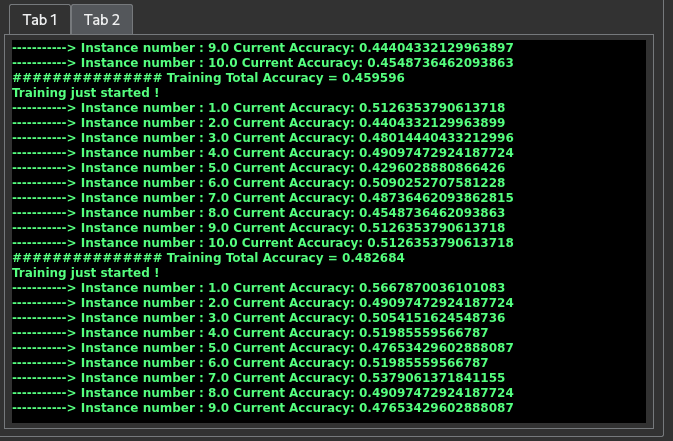
\includegraphics[scale=0.40]{gui_train_logs}
				\caption{Logarea progresului antrenării.}\label{Fig:gui_train_logs}
			\end{minipage}\hfill
		\hspace{1.9cm}
			\begin{minipage}{0.60\textwidth}
				\centering
				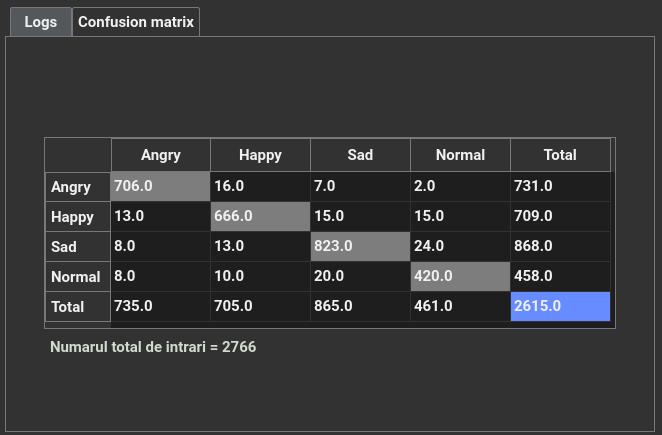
\includegraphics[scale=0.383]{gui_train_tabel}
				\caption{Matricea de confuzie a clasificatorului.}\label{Fig:gui_train_table}
			\end{minipage}
		\end{figure} 
		\subsection{Interfața grafică în modul de infererența}
		Modul de utilizare inferențial este disponibil doar pentru extragerea datelor în varianta end-to-end. Din cauza limitărilor impuse de folosirea extragerii caracteristicilor în modul "hand-crafted", prezentate de-a lungul lucrării, nu am putut garanta că setul de caracteristici propus reușește să cuprindă în totalitate informația emoțională. Astfel extragerea datelor în varianta "hand-crafted" este folosită doar pentru antrenare, ca un reper pentru varianta propusă, end-to-end. \par
		
		Interfața grafică este prezentată în Fig. \ref{fig:gui_inf}. După cum se poate observa după apăsarea butonului \textit{Inference}
		aplicația dezactivează toate funcționalitățile aferente modului de antrenare și le activează pe cele din modul inferență. În acest mod utlizatorul are posibilitatea să determine emoția din fișiere pre-înregistrate sau să își înregistreze pe loc propriile discursuri care vor fi clasificate automat după oprirea înregistrării. \par
		
		În spațiul textului editabil \textit{Folder path} utilizatorul poate să introducă calea pentru directorul în care se află fișierele audio pre-înregistrate pe care dorește să le clasifice. În mod implicit directorul folosit se numește "Inference" și este inclus în directorul în care se află proiectul. Combo box-ul \textit{File} enumeră toate fișierele audio cu extensia .wav din acel director. Prin apăsarea butonului \textit{Play} din dreapta acesteia utilizatorul poate auzi înregistrarea pe care dorește să o clasifice. Pentru clasificare însă, este nevoie că utilizatorul să aleagă fișierul dorit și apoi să apese pe butonul \textit{Start}. În urma acestui șir de comenzi probabilitățile aferente emoțiilor clasificate vor fi ilustrate in barele de progres \textit{Angry},  \textit{Happy}, \textit{Sad} și \textit{Neutral}. \par
		Recunoașterea emoției în timp real este posibilă prin apăsarea butonului \textit{Record}. Odată apăsat acest buton, aplicația va începe să înregistreze prin microfonul implicit al calculatorului. Când utilizatorul a terminat de înregistrat discursul pe care dorește să îl clasifice, pentru a determina emoția, utilizatorul trebuie să apese butonul \textit{Stop}. Butonul \textit{Stop} va opri firul de execuție pentru inregistrare, va salva discursul într-un fișier audio și va oferi înregistrarea obținută modelului pentru clasificare. Ca și în cazul anterior, distribuția de probabilitate a emoțiilor va fi prezentată grafic în barele de progres aferente. \par
		\begin{figure}[h]
			\hspace{-0.7cm}
			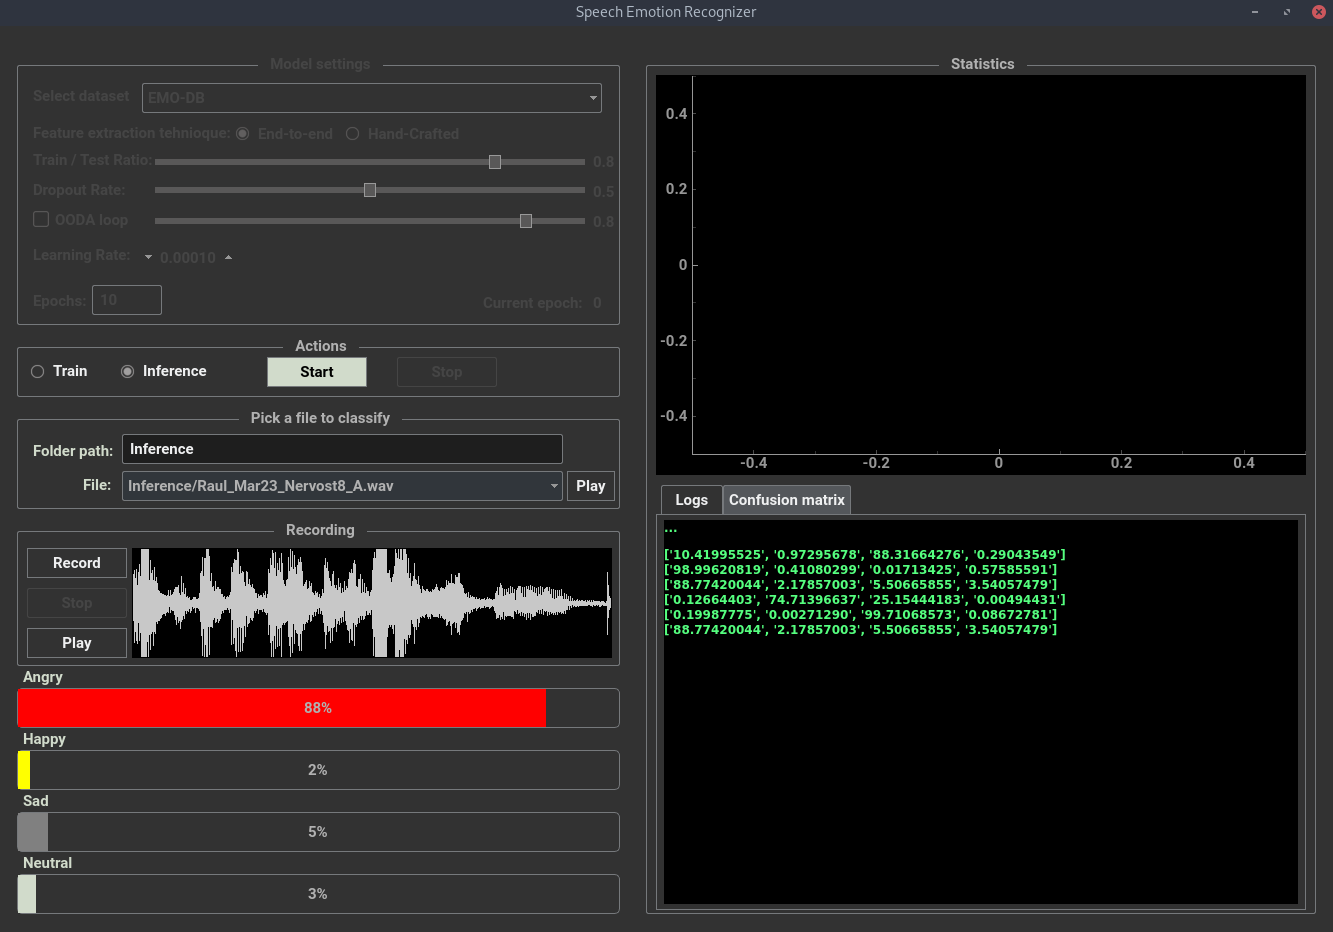
\includegraphics[scale=0.40]{gui_inf}
			\caption{Interfața grafică în modul de inferență}
			\label{fig:gui_inf}
		\end{figure} 
		În timpul înregistrării semnalul audio va fi proiectat în timp real în interfața grafică. Pentru a continua înregistrarea și a actualiza interfața grafică în același timp, după apăsarea butonului \textit{Record} se crează un nou fir de execuție special pentru procesul de înregistrare, asemănător cu crearea unui nou fir de execuție pentru procesul de antrenare prezentat în sub-capitolul \ref{guiAntrenare}. Inregistrearea semnalului audio este realizată folosind librăria PyAudio iar proiectarea semnalului inregitrat este realizată prin memorarea unui set de amplitudini ale acestuia și proiectarea lor folosind librăria PyQt5 la o frecvență calculată în funcție de rata de eșantionare a semnalului. \par
		În timpul înregistrării pot există momente de liniște prelungite care dacă persistă pot influența precizia clasificatorului. Pentru a reduce aceste momente la un minim s-a folosit librăria webrtcvad, care conține metode capabile să determine existența unui discurs într-un segment audio folosindu-se de anumite formule matematice asemănătoare cu cele prezentate în \ref{mel}. Secvența de cod care realizează înregistrarea și această filtrare a vocii umane este ilustrată mai jos.
		\begin{lstlisting}[language=Python, caption={Initializarea fluxului de transmitere a datelor pentru inregistrarea}]	
self.stream = pyaudio.PyAudio().open(format=self.sample_format,
									channels=self.channels,
									rate=self.rate,
									input=True,
									frames_per_buffer=self.chunk_size, 
									stream_callback=self.process_new_frame)

self.vad = webrtcvad.Vad()
self.vad.set_mode(1) \end{lstlisting}
		Funcția \textit{open} a librăriei PyAudio pornește un flux de date provenite de la microfon, care după ce atinge un număr de segmente egal cu valoarea \textit{self.chunk\_size} îl transmite metodei \textit{self.process\_new\_frame}. Deoarece aceste linii de cod realizează funcția de înregistrare, valoarea parametrului \textit{input} este setată pe adevărat. Pentru a face funcția opusă, ascultarea unui fișier audio, fluxul de date este creat aproximativ în aceași metodă, modificandu-se valoarea parametrului input pe fals și setarea valoii parametrului output pe adevărat. \par
		
		În câmpul \textit{self.vad} se stochează o instanța a mecanismului de detectare a vocii și se setează drasticitatea filturlui pe valoarea 1, unde intervalul de agresivitate al acestuia este [0, 3]. \par

\begin{lstlisting}[language=Python, caption={Procesarea unui nou segmente al semnalului audio inregistrat. Daca segmentul nu contine discurs uman este exclus din inregistrarea finala.}]		
def process_new_frame(self, data, frame_count, time_info, status):
	data = np.frombuffer(data, dtype=np.int16)
	with self.lock:
		if self.vad.is_speech(data, self.rate):
			self.frames.append(data)
		if self._print_frames_count == self._print_chunk_size:
			self.thread.print_recording_signal.emit(self._print_frames)
			self._print_frames = np.array([])
			self._print_frames_count = 0
		else:
			self._print_frames = np.concatenate((self._print_frames,data), axis=0)
			self._print_frames_count+=1
		if self.stop:
			return None, pyaudio.paComplete
return None, pyaudio.paContinue	\end{lstlisting}
		Metoda \textit{process\_new\_frame} primește în parametrul \textit{data} un set de segmente audio de lungime \textit{frame\_count}. Aceste segmente sunt verificate de mecanismul de detecție prin metoda \textit{self.vad.is\_speech} și în caz pozitiv sunt adăugate la setul de segmente care urmează să fie clasificate de sistemul SER. \par
		Semnalul audio înregistrat este proiectat în interfața grafică prin folosirea metodei \textit{emit} a semnalului firului de execuție de înregistrare \textit{self.thread.print\_recording\_signal}. În vectorul \textit{self.\_print\_frames} sunt salvate toate segmentele primite pentru a afișa întregul semnal în interfața audio. \par
		La apăsarea butonului Stop din interfața grafică, câmpul \textit{self.stop} va opri procesul de înregistrare generând salvarea semnalului într-un fișier audio de tip .wav și pornirea clasificatorului.
		
		 
%---------------------------------------------------------------------------------------------------------------------------------------------		
		\chapter{Rezultate si experimente} \label{rezultate}
		 
		 În acest capitol vor fi prezentate rezultatele obținute în urma executării unui set de experminente prin care soluția propusă este testată în diferite configurații. Rezultatele obținute sunt apoi comparate cu cele ale altor arhitecturi din domeniu. Deși sistemul SER a fost implementat special pentru lucrul cu mai multe baze de date într-o manieră "end-to-end", rezultatele obținute atât în cazurile în care s-a folosit o singură baza de date cât și în cele în care extragerea datelor a fost de tip "hand-crafted" se mențin la nivelul celorlalte soluții SER.\par
		 
		 Soluția propusă în această lucrare de diplomă este antrenată într-o manieră "multi-domain", pe înregistrări care provin din baze de date diferite. Antrenarea "multi-domain" prezintă o serie de avantaje enumerate la \ref{datasets}, dar face ca compararea arhitecturii cu alte sisteme SER să fie dificilă. Din acest motiv, în continuare vor fi enumerate rezultatele obținute de model în particular pentru unele din bazele de date care alcătuiesc setul descris la \ref{datasets}. \par
		 Antrenând modelul pe întreaga bază de date EMO-DB \cite{emodb}, cu înregistrări aferente a 7 emoții, acuratețea maximă înregistrată a fost de 77\%, în timp ce acuratețea medie a fost de aproximativ 75\%. Aceste rezultate sunt comparative cu cele obținute de Kerkeni et al., 2018 \cite{comp1}, unde folosind un modul clasificator similar, două celule recurente LSTM urmate de două nivele dense, s-a obținut o acuratețe maximă de 73\% și una medie de 69.55\%. Una din cele mai de succes soluții SER antrenate pe această baza de date este prezentată în Issa et al, 2020 \cite{comp2}, unde numărul înregistrărilor a fost mărit prin folosirea unor tehnici de augmentare ca adăugarea unui nou set de exemple obținut prin accelerarea la 1.23\% a înregistrărilor, incetinrea la 0.81\%, mutarea punctului de start, sau adăugarea unui zgomot la 25\% din lungimea înregistrării. În urma acestei serii de augmentari, acuratețea modelului propus în Issa et al, 2020 \cite{comp2} a atins precizia de 82.86\%.\par
		 Baza de date RAVDESS \cite{ravdess} conține 1440 de înregistrări incorporând 8 emoțîi. Folosind înregistrări doar din acesată baze date pentru antrenare, modelul propus a obținut o acuratețe maximă de 71.08\% și una medie de 68\%. Acest rezultat este comparativ cu precizia înregistrată în Issa et al, 2020 \cite{comp2} de 71.61\%. Zeng et al., 2017 \cite{comp3} au obținut o acuratețe de 65.97\% folosind rețele neuronale produnde și o antrenare tip "multi-task", antrenând modelul să clasifice emoții atât în vorbire cât și în cântece. Folosind un model clasficator bazat pe rețele neuronale convoluționale Popova et al., 2018 \cite{comp4} au înregistrat o acuratețe de 71\% pe această baze de date. \par
		 Realizând antrenarea calsificatorului pe 7 emoțîi folosind înregistrări din baza de date EMOVO \cite{emovo} s-a atins o acuratețe maximă de 70\%. Rezultate similare au fost obținute și în Latif et al., 2018 \cite{comp5}, acuratețe de 76.22\%, unde clasificatorul sistemului SER a fost bazat pe o tipologie specială de rețele neuronale numite "Deep Belief Neural Networks". Latif et al., 2018 \cite{comp5} propun și folosirea tehnicii "transfer learning", prezentată la \ref{tehnici}, unde înaintea antrenarii pe baza de date EMOVO modelul este antrenat mai întâi pe baze de date din alte limbi. Această tehnică ii permite modelului să depășească valoarea inițială a acurateții atingând precizia de 80\%. \par 
		 Antrenând soluția propusă în această lucrare pe baza de date ENTERFACE'05 \cite{enterface}, care conține înregistrări reprezentative pentru un set de 6 emoții, acuratețea maximă obținută a fost 83.26\%. Rezultate similare au fost obținute în Schuller, 2011 \cite{comp6}, unde prin folosirea uni clasifiator tradițional pentru probmela recunoașterii emoției, "Support Vector Machine", s-a atins o precizie de 62.8\% pe această baza de date. Rezultate mai promițătoare au fost obținute în Ooi et al., 2014 \cite{comp7}, în care modelul propus înregistrează precizia 75.89\%. \par
		 După cum se poate observa, chiar dacă soluția propusă este de tip "multi-domain", rezultatele obținute de sistemul SER implementat în această lucrare se apropie considerabil de cele obținute de implementări care sunt specializate pe câte una din acestea. Prin reducerea numărului de exemple pentru a cuprinde doar setul de emoții enumerat la \ref{solutie} (fericire, tristețe, enervare și neutru), acuratețea pe fiecare din bazele de date depășește rezultatele prezentate mai sus. În cazul bazei de date EMO-DB acuratețea maximă obținută pe cele 4 este de 91.04\%, în cazul RAVDESS 76.11\%, EMOVO 80.59\% și ENTERFACE'05 90.05\%.  
		 
		 \par		 
		 Un alt experiment a fost realizat prin modificare modului de extragere a caracteristicilor de intrare. Metoda "end-to-end", \ref{end-to-end}, este cea propusă pentru arhitectura finală a sistemului SER implementat în această lucrare, totuși pentru a evidenția importanța acestei tehnici în continuare vor fi prezentate rezultatele înregistrate pentru clasificare bazată pe caracteristici "hand-crafted". Acuratețea maximă înregistrată în cadrul acestui experiment a fost de 68.56\%, iar acuratețea medie a fost de 67\%.
		 
		 \par
		 Soluția propusă cuprinde atât o antrenare tip "multi-domain" cât și o extragere a caracteristicilor de intrare "end-to-end". Rezultatele obținute folosind această configurație finală sunt încurajatoare fiind asemănătoare cu cele obținute de o altă arhitectură SER antrenată într-o modalitate similară. Acuratețea ne-ponderată maximă obținută de modelul propus în această lucrare a fost de 84.1\%, având o valoare medie de aproximativ 82\%. Aceste rezultate le depășesc cu aproximativ 15\% pe cele obținute folosind caracteristicile "hand-crafted", subliniind beneficiile extragerii "end-to-end". În același timp, deși era de așteptat că acuratețea modelului să scadă folosind mai multe baze de date, se poate observă cum această se menține, și chiar depășește, unele din preciziile înregistrare pe unele din bazele de date. Sistemul SER prezentat în Milner et al., 2019 \cite{multi-domain} profită de generalitatea obținută prin antrenarea "mulți-domain" într-o arhitectură SER similară cu cea implementată în această lucrare, \ref{prez_multi_domain}. Acurateța ne-ponderată obținută în acest studiu a fost de 82.26\% pe 6 emoții diferite, fiind apropiată de cea obținută de mine chiar dacă setul de baze de date și numărul de emoții clasificate diferă. \par		 
		 
		 Din punct de vedere arhitectural soluția propusă poate fi comparată cu alte câteva din domeniul SER. Folosind o singură baza de date, dar același mod de extragere a caracteristicilor de intrare, soluția prezentată în Li, Yuanchao et al., 2019 \cite{yuan}, a atins o precizie de 82.8\%, fiind una dintre cele mai înalte măsurate pe baza de date IEMOCAP \cite{iemocap}. Misramadi et al., 2017 \cite{misramadi}, au introdus un modul clasificator bazat pe rețele neuronale recurente bidirecționale combinate cu un mecanism de atenție, similar cu cel din acest proiect, și au obținut o acuratețe cu 3.1\% mai mare decâtcea înregistrată până în acel moment pe baza de date folosită de aceștia. Alte rezultate cu arhitecturi apropiate de cea propusă de mine au fost:  Kerkeni et al. (2018) \cite{compar1} unde s-a înregistrat o acuratețe de 82.14\% pe baza de date EMO-DB \cite{emodb}, Fonnegra et al., 2018 \cite{compar2} au obținut rezultate promițătoare folosind baza de date ENTERFACE'05 \cite{enterface} cu o acuratețe 92\%, Lim et al., 2016 \cite{compar3} au executat mai multe experminete pe baza de date EMO-DB \cite{emodb} obținând precizii de 87.74\% într-o arhitectură cu rețele convoluționale, 79.87\% într-o arhitectură cu rețele neuronale recurente și 88.01\% combinând cele două tipologii de rețele neuronale într-o manieră asemănătoare cu arhitectura folosită în această lucrare de diplomă. \par
		 
		 Alte experimente au fost realizate pentru a se încerca reducerea timpului de antrenare al modelului păstrând însă o eroare tolerabilă. Prin folosirea ciclurilor OODA, \ref{ooda}, la un anumit număr de epocii se extrage un set de exemple de antrenare până se atinge proporția rămasă dorită. Setul de exemple extrase a fos deteminat în două moduri: în funcție de eroarea fiecărei înregistrări și aleatoriu. În primul caz diferența dintre acuratețea înregistrată și cea din modul de antrenare normal este mult prea mare, obținând o precizie de maxim 71\% și una medie de 68\%. Cel de al doilea caz prezintă rezultate mai promițătoare, acuratețea maximă înregistrată fiind de 80\% iar cea medie de 78\%. Timpul de antrenare cu un număr de 80 de epocii este redus la 3 ore și 30 de minute de la 5 ore in cazul folosirii întregului set din baza de date. Aceste rezultate au permis introducerea unui nou mod de antrenare "rapid" prin care modelul își păstrează arhitectura inițială iar precizia se menține la un nivel satisfăcător. Acest mod de învățare este unul opțional fiind adresat utilizatorilor care nu pot aștepte întreagă durata necesară antrenării.
%---------------------------------------------------------------------------------------------------------------------------------------------		 
		\chapter{Concluzii}		
		Lucrarea de diplomă conține atât o soluție pentru recunoașterea emoției în vorbire cât și o interfață grafică care permite antrenarea, testarea și inferența eficientă a sistemului SER. Domeniul recunoașterii emoției în vorbire nu este până în acest moment unul "cucerit", prezentând o gama largă de obstacole care nu au permis obținerea unei acurateți destul de satisfăcătoare pentru a permite acestor algoritmi să fie introduși pe piață. Totuși, soluția implementată de mine reușește să atingă o acuratețe comparabilă cu a unor arhitecturi de success din domeniu și chiar să le depășească în anumite configurații. Această acuratețe este pusă apoi în practică prin interfață grafică care permite utilizatorului să clasifice emoțiile din interiorul discursurilor provenite din mai multe surse. \par		
		
		Sistemul SER propus încearcă să determine o arhitectură eficientă pentru rezolvarea recunoașterii de emoții în vorbire intergrand diferite tehnici și concepte cu scopul de a cuprinde cât mai complet complexitatea problemei. Alegerea folosirii unui set de mai multe baze de date este justificată de îmbunătățirea generalității modelului "Machine Learning". Extragerea datelor în manieră "end-to-end" este motivată de lipsa unui set de caracteristici audio de intrare specializat pe recunoașterea emoțiilor în vorbire. Implementarea unui modul clasificator bazat pe rețele neuronale recurente este aleasă pentru a profita de relațiile temporale între emoțiile din segmente audio aflate la momente diferite. Urmarea rețelei recurente de un mecanism de atenție este bazată pe filtrarea segmentelor lipsite de emoție pentru a reduce inconsistențele introduse de acestea. \par
		
		În construirea acestui proiect am folosit multe din tehnicile învățate în decursul facultății de Automatică și Calculatoare, ca programarea orientată pe obiecte, dezvoltarea interfetelor grafice, programarea concurență și diferite concepte ale inteligenței artificiale. Totuși, pentru realizarea unui sistem SER am necesitat informații specifice care au fost obținute prin studiul unor articole stintifice din domeniu, enumerate în decursul lucrării. Tehnologiile folosite au crescut în număr cu mulțimea de functinalitati adăugate incluzând limbajul de programare Python, celebra librărie Tensorflow pentru dezvoltarea aplicațiilor "Machine Learning", Librosa pentru extragerea informațiilor auditive, webrtcvad pentru identificarea semgentelor care conțin voce umană și pyaudio pentru înregistrarea și redarea fișierelor audio. \par
		
		Scopul final al unui sistem SER este acela de a fi introdus în interfețele de comunicare om-mașină din viitor, pentru a oferii mașinilor capacitatea de a înțelege conversațiile la care iau parte și dintr-un context emoțional. Integrarea acestor algoritmi va crește calitatea conversațiilor permițând ca interfețele de comunicare om-mașină să atingă o calitate asemănătoare cu cele de la om la om. Până a ajunge în acel punct însă, algoritmii de recunoaștere a emoțiilor trebuie să mai treacă printr-o serie de imbunatariri pentru a crește gradual acuratețea înregistrată. Soluția propusă de mine reprezintă o arhitectură într-o stare incipientă, având potențialul de a fi extinsă prin introducerea mai multor tehnici. \par
		
		Prima modalitate de îmbunătățire a sistemului SER propus, și cea mai simplă, ar fi mărirea numărului de baze de date folosite pentru a amplifica și mai mult generalitatea modelului, să combată problema numărului redus de exemple și să mărească numărul de emoții clasificate. \par 
		O altă modificare ar putea fi constituită de introducerea unui modul care să diminueze diferențele dintre înregistrările provenite din baze de date diferite. Algoritmi care realizează această sarcina au fost deja introduși în alte soluții din domeniu. De exemplu Deng et al. , 2014 \cite{imbun1} au folosit cu succes o tehnică numită "adaptive denoising-autoencoders", care învață să determine și să elimine diferențele dintre mai multe baze de date prin aducerea înregistrărilor acestora la o formă asemănătoare cu cele dintr-o anumită baza de date țintă. Alte tehinici de reducere a discrepanțelor bazelor de date sunt normalizarea per baza de date sau normalizare per vorbitor, Bjorn et al, 2010 \cite{spnorm}. \par
		Tehinca antrenării pe mai multe sarcini, "multi-task", poate la rândul ei să aducă imbunatațiri puternice modelului clasificator. Prin antrenarea modelului pe o serie de sarcini în același timp sistemul poate să devină inflexibil la variații ale semnalului audio care nu ar trebui să influențeze emoția clasificată. Li, Yuanchao et al., 2019 \cite{yuan} au antrenat arhitectură SER popusa atât pe recunoașterea emoțiilor în vorbire cât și pe determinarea sexului vorbitorului, în timp ce Milner et al., 2019 \cite{multi-domain} au folosit ca sarcină secundară determinarea bazei de date din care face parte înregistrarea curentă. Aceste două tehnici s-au dovedit a fi avantajoase în combatarea influenței sexului vorbitorului cât și a bazei de date de proveniență în decursul procesului de clasificare.\par 
		O altă extindere a proiectului curent ar putea fi combinarea soluției propuse cu un algoritm de detecție a emoției vizuale. Astfel produsul final va putea determina emoția umană folosindu-se de două tipuri diferite de stimului. Această metodă s-a demonstratat a fi avantajoasă în difeite articole că Tzirakis et al., 2014 \cite{tzir} sau Sana et al., 2010 \cite{imbun3}, unde s-a depășit acuratețea sistemului SER inițială prin adăugarea informației vizuale în clasificarea emoțiilor. \par
		
		
		Proiectul meu de diplomă prezintă astfel o soluție incipientă pentru una din problemele care au rămas încă nerezolvate în domeniul inteligenței artificiale, recunoașterea emoției în vorbire. Lucrarea de diplomă include atât un model "Machine Learning" clasificator cât și o interfață grafică care permite utilizatorului să încerce diferite configurații de parametrii, să observe statistici detaliate ale proceselor care i-au parte în timpul antrenării și să încerce modelul antrenat pe înregistrări din diferite surse. Chiar dacă sistemul SER prezentat nu este momentan viabil pentru a fi introdus pe piață rezultatele obținute sunt comparative cu cele ale unora dintre cele mai de succes implementari din domeniul recunoașterii de emoții în vorbire din prezent. Rezultatele obținute sunt încurajatoare si susțin faptul că soluția "Machine Learning" propusă are in viitor potențialul de a depașii precizia curentă prin aplciarea unei game largi de tehnici deja exisitente sau a unora noi, care tind să apară anual în acest domeniu.		
			
		\renewcommand{\clearpage}{}
		\addcontentsline{toc}{chapter}{Bibliografie}
		\printbibliography[title={Bibliografie},notcategory=cited,resetnumbers=true]
		%\hfil \\
		%\hfil \\
		\addcontentsline{toc}{chapter}{Referinte}
		\printbibliography[title={Referinte},category=cited,resetnumbers=true]
		\newpage
\end{document}




























